\documentclass[shortabstract,inz]{iithesis}

\usepackage[utf8]{inputenc}

\polishtitle    {Infrastruktura do zarządzania urządzeniami i sterownikami urządzeń 
w systemie operacyjnym FreeBSD z częściową implementacją w systemie operacyjnym Mimiker}

\englishtitle   {The device and device drivers infrastructure in FreeBSD operating system 
with partial implementation in Mimiker operating system}

\polishabstract {System komputerowy nie jest niepodzielną jednostką
  funkcjonalną.  Składa się na niego wiele, często bardzo różnych,
  urządzeń wymagających odmiennego traktowania.  Szczególne
  traktowanie każdego urządzenia z osobna wprowadzałoby chaos, stąd
  potrzeba spójnego podsystemu zarządzającego szeroką gamą urządzeń w
  jednolity sposób. \fmlinebreak W tej pracy opisaliśmy organizację
  systemu komputerowego,
  rodzaje urządzeń oraz sposoby ich połączenia.
  Przedstawiamy również jeden ze sposobów zarządzania urządzeniami i
  ich sterownikami - podsystem NewBus systemu operacyjnego FreeBSD.
  Omówimy proces wykrywania i inicjalizacji urządzeń,
  ich organizację w systemie operacyjnym oraz rezerwację zasobów
  sprzętowych. Na koniec przedstawimy implementację infrastruktury do
  zarządzania urządzeniami w systemie operacyjnym Mimiker wzorowaną na
  infrastrukturze NewBus.}

\englishabstract{Computer system is not an indivisible functional unit.
It is made of many, often very different devices, requiring different handling.
Special treatment of every device in a system would cause chaos, thus need for
consistent subsystem responsible for handling a wide range of devices in an unified way. \fmlinebreak
In this paper, we described computer system structure, types of devices and ways they are connected.
We present one way of managing devices and their drivers - NewBus subsystem in FreeBSD operating
system. We will discuss process of detecting and initializing devices, their organization in 
operating system and hardware resources reservation. At the end we will present implementation of 
infrastructure responsible for handling devices in Mimiker operating system inspired by NewBus infrastructure.}

\author         {Jan Mazur \and Wojciech Moczulski}
\advisor        {dr Piotr Witkowski}
\date          {3 września 2018}
\advisorgen    {dr. Piotra Witkowskiego}

% \usepackage{graphicx,listings,amsmath,amssymb,amsthm,amsfonts,tikz}
\usepackage{graphicx}
\usepackage[T1]{fontenc}
\usepackage{tablefootnote}

\graphicspath{ {images/} }

\usepackage{amsfonts, listings}

\lstset{
    basicstyle=\ttfamily\small,
    numberstyle=\footnotesize,
    numbers=left,
    frame=single,
    extendedchars=true,
    literate={ą}{{\k{a}}}1 {Ą}{{\k{A}}}1 {ę}{{\k{e}}}1 {Ę}{{\k{E}}}1 {ó}{{\'o}}1 {Ó}{{\'O}}1 {ś}{{\'s}}1 {Ś}{{\'S}}1
             {ł}{{\l{}}}1 {Ł}{{\L{}}}1 {ż}{{\.z}}1 {Ż}{{\.Z}}1 {ź}{{\'z}}1 {Ź}{{\'Z}}1 {ć}{{\'c}}1 {Ć}{{\'C}}1
             {ń}{{\'n}}1 {Ń}{{\'N}}1
}

\begin{document}

\chapter{Wprowadzenie}
\section{Czym jest komputer? Rola urządzeń zewnętrznych} % JM

Komputer z założenia jest programowalną maszyną liczącą. Oznacza to, że potrafi
przeprowadzać obliczenia na podstawie podanych przez użytkownika instrukcji.
Instrukcje te muszą w wyczerpujący sposób opisywać obliczenia które mają zostać wykonane,
oraz muszą być podane w sposób możliwy do zinterpretowania przez maszynę.
Na przykład zakodowane przy pomocy tablic programowych, kart perforowanych, 
taśm magnetycznych, bądź zadane z użyciem dalekopisu.
Maszyna po zdekodowaniu instrukcji, bez ingerencji człowieka, przeprowadza obliczenia.
Gdy obliczenia się zakończą, ich wynik powinien być przekazany użytkownikowi, na przykład
poprzez te same media, które służyły do przekazania wejściowych instrukcji maszynie.

W podobny do wyżej opisanego sposób, John von Neumann w 1945 roku zdefiniował
działanie \textit{automatycznego systemu liczącego}\cite{paper:neumann}. 
W tak działającej maszynie naturalnym wydało mu się wyodrębnienie
kilku komponentów, z których każdy miał ściśle określone zadanie.
Wśród komponentów były takie jak jednostka licząca, jednostka kontrolna, pamięć, oraz moduły
odpowiedzialne za pobieranie instrukcji zakodowanych na zewnętrznych
dla maszyny nośnikach i zapisywanie na tychże nośnikach wyników
obliczeń.

W opisanej przez Neumanna architekturze urządzenia spełniają rolę
interfejsu pomiędzy maszyną, a człowiekiem. Służą do obustronnej
komunikacji, pozwalają zdefiniować dane wejściowe, a następnie po
skończonych obliczeniach prezentują dane wyjściowe. Prawdopodobnie stąd nazwa
\textbf{urządzenia wejścia-wyjścia (ang. I/O devices, Input/Output devices)}.

Aby prowadzić interakcję z jednostką liczącą, urządzenia tego typu są niezbędne.

\begin{figure}
\begin{center}
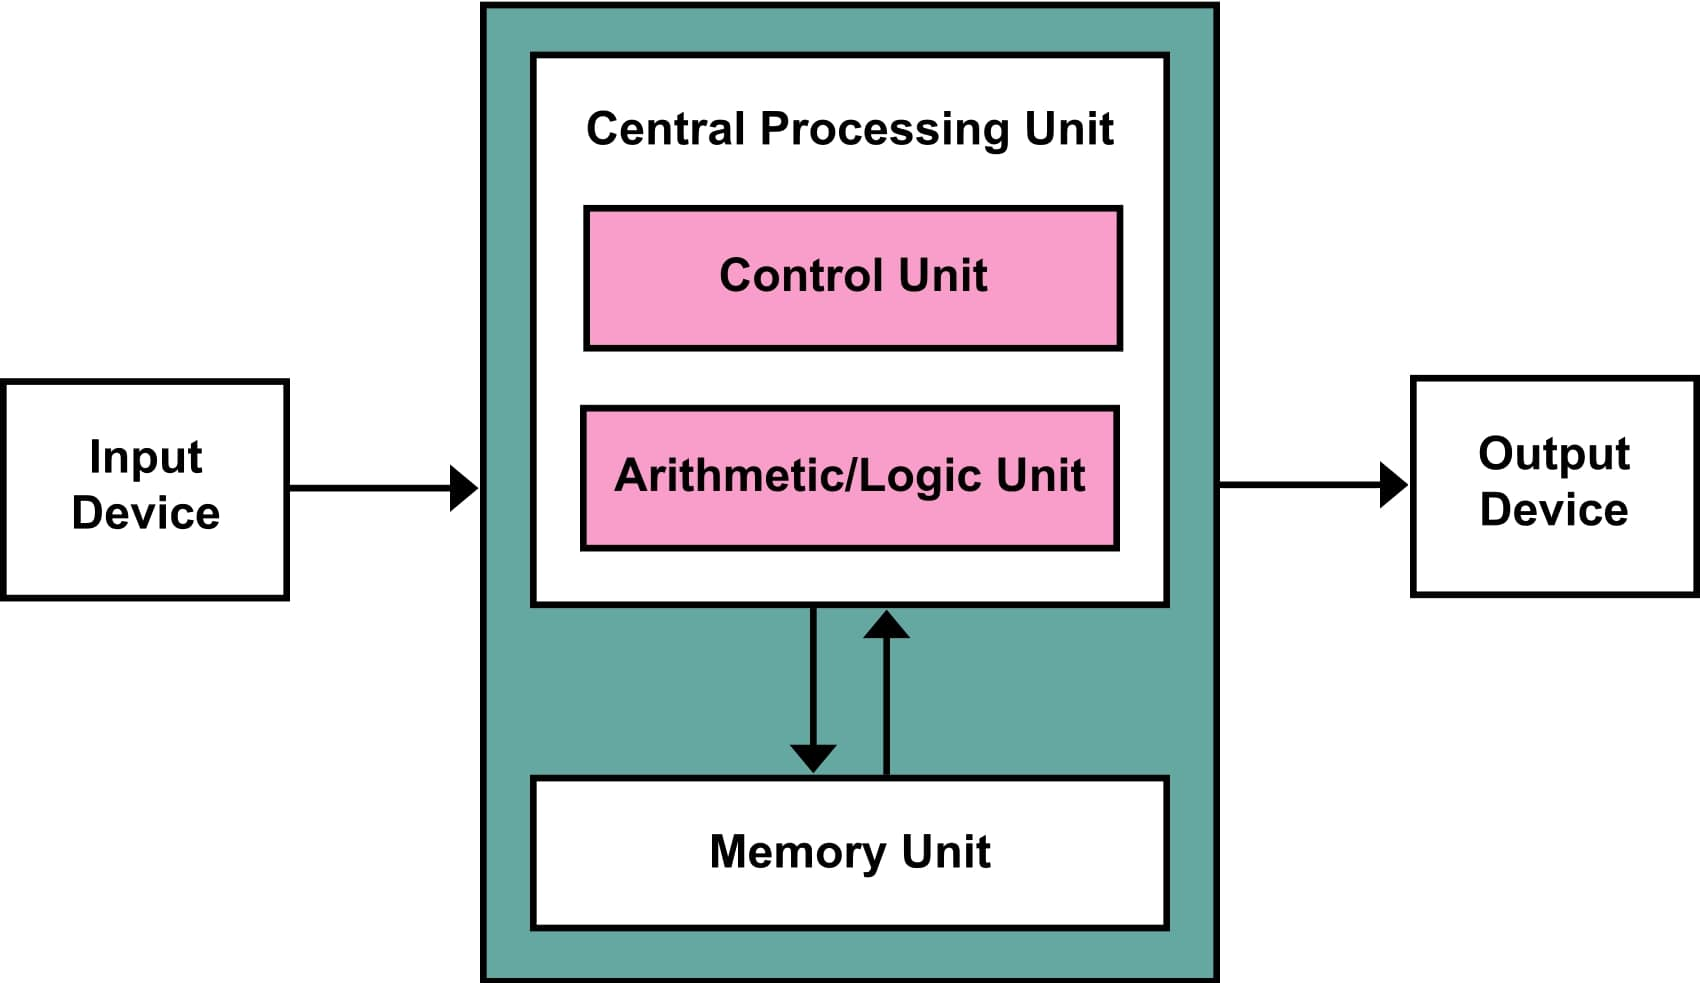
\includegraphics[width=\linewidth/2]{Von_Neumann_Architecture}
\caption{Uproszczony schemat architektury von
  Neumanna \cite{image:von_neumann}}
\label{fig:von_neumann}
\end{center}
\end{figure}
% https://commons.wikimedia.org/wiki/File:Von_Neumann_Architecture.svg

Mimo upływu ponad 70 lat, wpływ Architektury von Neumanna dalej jest
widoczny w nowoczesnych systemach komputerowych.

\section{Rozwój urządzeń} % JM
% Tanenbaum historia 
% Tanenbaum  hardware

Postęp technologiczny sprawiał, że komputery stawały się
coraz bardziej interaktywne, pozwalały na większą swobodę interakcji z
użytkownikiem niż systemy z przetwarzaniem wsadowym \cite{wiki:batch_processing}\cite{book:tanenbaum_history}.

Pierwsze systemy operacyjne z podziałem czasu (ang. timesharing) \cite{wiki:timesharing},
Potrafiły obsługiwać wiele urządzeń wejścia-wyjścia pracujących na rzecz
wielu różnych użytkowników jednocześnie.
Potrzeba trwałego przechowywania danych spowodowała pojawienie się
urządzeń pamięci masowej. Począwszy od nośników magnetycznych, przez
optyczne na dyskach półprzewodnikowych kończąc.

Z czasem cena komputera jak i jego wielkość drastycznie się zmniejszyły. Dawniej 
komputer zajmował powierzchnię sporego pomieszczenia.
Już nie tylko wielkie korporacje i instytucje rządowe mogły sobie pozwolić na 
posiadanie zaawansowanej maszyny obliczeniowej ale także osoby prywatne.
Tak powstały \textbf{komputery osobiste (ang. Personal Computer - PC)}.

Aby komputery były coraz bardziej powszechne i dostępne, nie mogły już wymagać
specjalnie wyszkolonych operatorów do ich obsługi. Potrzebne były dużo prostsze
metody interakcji, tak aby jak najwięcej osób w krótkim czasie mogło nauczyć się
obsługi komputera.
Wymagało to zarówno rozwoju oprogramowania (szczególnie systemu operacyjnego), 
jak i sprzętu.

Archaiczne, drogie, często skomplikowane i nieporęczne już urządzenia wejścia-wyjścia 
takie jak te wymienione wcześniej, zostały zastąpione przez
klawiatury, monitory, ekrany dotykowe, czy nawet systemy interakcji głosowej i wizualnej.

Każdy kolejny etap rozwoju urządzeń sprawiał, że stawały się one coraz bardziej skomplikowane,
a tym samym złożoność sprzętowych i programowych mechanizmów ich obsługi rosła.

Komputery PC \cite{pleonazm} wyrosły na wysoce modularne systemy, w których użytkownik może
z powodzeniem modyfikować możliwości swojej maszyny poprzez podłączenie
urządzenia na karcie rozszerzeń obsługującej pewien ustalony protokół komunikacji.
Urządzenia peryferyjne stały się naturalnym sposobem an rozszerzanie
możliwości systemu. Liczba urządzeń jest w zasadzie
nieograniczona, a każde z nich musi być odpowiednio obsłużone przez
system.

Każde nowe urządzenie, którego maszyna ma być być świadoma, z którym
wymienia dane, musi być odpowiednio oprogramowane. Kod obsługujący
dane urządzenie nazywamy \textbf{sterownikiem urządzenia}. Jednakże
sterowniki nie obsługują urządzeń bezpośrednio.
Wchodzą one w interakcję z układem (bądź zbiorem układów elektronicznych) zwanym
\textbf{kontrolerem}. Pośredniczą one w komunikacji między systemem
operacyjnym a konkretnym urządzeniem (lub zbiorem urządzeń) oferując systemowi operacyjnemu
przystępniejszy protokół komunikacji (wciąż jednak bardzo złożony) \cite{book:tanenbaum_hardware}.


\section{Kontrolery} % JM
\label{sec:kontrolery}
% https://simple.wikipedia.org/wiki/Device_controller
% Tanenbaum

Urządzenia z czasem stawały się coraz bardziej skomplikowane, stąd
również komunikacja z nimi stawała się bardziej zawiła. 
Aby masowo produkować urządzenia w łatwy sposób rozszerzające możliwości
komputera, wprowadzono standardy komunikacji z urządzeniami.
Np. dowolny kontroler dysku SATA \cite{sata} powinien obsłużyć dowolny dysk SATA.

Obecnie niemal każde urządzenie wejścia-wyjścia jest podłączone do
systemu komputerowego za pośrednictwem układu zwanego \textbf{kontrolerem}
którego zadaniem jest udostępnienie systemowi operacyjnemu
prostszego interfejsu (który pomimo wszystko jest bardzo złożony)
komunikacyjnego z urządzeniem zewnętrznym \cite{wiki:controller}\cite{book:tanenbaum_hardware}.
 
Kontroler natomiast komunikuje się z
urządzeniem poprzez ustandaryzowany protokół danego typu \textbf{magistrali}, taki jak
na przykład nie używane już SCSI \cite{scsi} i ATA/IDE \cite{ata_ide}, czy powszechnie występujące
PCI i USB, przybliżone w rozdziałach \ref{sec:pci} i \ref{sec:usb}.
% https://en.wikipedia.org/wiki/SCSI
% https://en.wikipedia.org/wiki/Parallel_ATA
% odnośnik do PCI w pracy
% odnośnik do USB w pracy

Sztandarowym przykładem zadania które pełni kontroler jest tłumaczenie
logicznych adresów bloków dyskowych \cite{book:memory_systems_chapter_18} 
(LBA) na adresowanie oparte na wyborze cylindra, sektora i głowicy (CHS) \cite{book:tanenbaum_dyski}. 
Konwersja ta nie należy do
trywialnych z tego powodu, że cylindry wewnętrzne mają mniej sektorów
od zewnętrznych, oraz ze względu na możliwe wystąpienie wadliwych
sektorów i ich przemapowanie na sektory poprawne.  Po wyznaczeniu
adresu CHS, kontroler dokonując odczytu bądź zapisu musi zmienić
położenie głowicy z cylindra nad którym obecnie się znajduje na
pozycję nad docelowym cylindrem. Następnie musi poczekać, aż docelowy
sektor w wyniku rotacji dysku przesunie się pod głowicę. Wtedy
wykonywany jest odczyt bądź zapis i liczone są sumy kontrolne. Logika
zawarta w kontrolerach przypomina niewielkie wbudowane komputery,
które zostały zaprogramowane przez dostawcę sprzętu do
wykonywania tej pracy.

Obecnie używane kontrolery najczęściej są zintegrowane z płytą główną, 
ale mogą być też podłączone do odpowiednich magistral jako karty rozszerzeń.

\section{Magistrale} % JM
% https://en.wikipedia.org/wiki/Bus_mastering
% https://www.mtholyoke.edu/courses/dstrahma/cs221/olr/olr11.htm
% https://whatis.techtarget.com/definition/bus-master
% https://en.wikipedia.org/wiki/Direct_memory_access


Urządzenia w systemie komputerowym wymagają odpowiedniej organizacji.
Muszą być ze sobą fizycznie połączone, aby wchodzić ze sobą w interakcję.
Służą do tego \textbf{magistrale} \cite{book:tanenbaum_hardware}.

\textbf{Magistralą} nazywamy \textit{zespół linii przenoszących sygnały oraz układów
wejścia-wyjścia służących do przesyłania sygnałów między połączonymi
urządzeniami w systemach mikroprocesorowych} \cite{wiki:magistrala_def}.

W większości magistral można wyodrębnić trzy podstawowe szyny (kanały, linie):
szynę sterującą (kontrolną), adresową i danych. Sygnały elektryczne na pierwszej
z nich interpretowane są jako wybór aktualnie podejmowanej akcji na magistrali, takiej jak
np. odczyt i zapis danych. Za pomocą szyny adresowej wybierane jest miejsce z, bądź do którego
będzie wykonywany transfer. 
Ostatnia szyna, jak sama nazwa wskazuje, służy do przesyłania danych.

Magistrale można podzielić ze względu na typ transmisji na \textbf{równoległe} (np. PCI [\ref{sec:pci}]) i \textbf{szeregowe} (np. PCI-express \cite{pcie}).
Pierwszy typ posiada wiele linii (przewodów), co pozwala na równoległą transmisję bitów słowa danych.
Trudnością jest zapewnienie dotarcia wszystkich bitów przesyłanej wiadomości w tym samym czasie.
W drugim przypadku wiadomości wysyłane są szeregowo, jednym pasmem (ang. lane), bit po bicie,
niczym pakiety w sieci ethernet.
Zazwyczaj używa się wielu równoległych pasm w połączeniu punkt-punkt \cite{wiki:point_point} (jak w PCI-express).
% odnośnik do "połączenie point-point"
% PCIe https://en.wikipedia.org/wiki/PCI_Express

Komunikacja między urządzeniami podłączonymi do magistrali musi być dobrze
zorganizowana. Wyobraźmy sobie telekonferencję wielu osób. Gdyby wszyscy mówili jednocześnie,
nikt nie byłby w stanie zrozumieć nikogo. Analogiczna sytuacja dotyczy magistral.

W przypadku, gdy więcej niż jedno urządzenie na magistrali może inicjować
transakcje potrzebny jest arbitraż. Standard
magistrali danego typu może specyfikować jak ma on wyglądać, 
bądź zezwalać na zewnętrzną implementację arbitra (np. w PCI \cite{pci_arbitration}).
% https://en.wikipedia.org/wiki/Conventional_PCI#Arbitration

Z magistralą najczęściej skojarzony jest kontroler potrafiący obsługiwać urządzenia danego typu.
Np. kontroler magistrali SATA potrafi obsługiwać wszystkie dyski SATA.
Kontrolerami, które wspomagają komunikację na magistrali są PIC i DMA, które
zostaną omówione w rozdziałach \ref{def:przerwania} i \ref{sec:dma}.

Urządzenie inicjujące transakcję, mające w danej chwili kontrolę nad magistralą
nazywamy \textbf{nadzorcą (ang. master)} \label{def:master/slave}. Pozostałe urządzenia nazywamy wtedy 
\textbf{podległymi (ang. slave)}.
% pci bus mastering http://www.pcguide.com/ref/mbsys/buses/types/pciMastering-c.html
% isa bus mastering http://www.hardwarebook.info/ISA#Bus_Mastering 


Większość magistrali o wysokiej przepustowości, pozwala każdemu urządzeniu
podłączonemu do niej, na inicjacje operacji \cite{pci_bus_mastering}. Mechanizm ten
nazywamy \textit{bus mastering}, \label{def:bus_mastering} bądź \textit{first-party DMA}.  Każde
urządzenie może ubiegać się o dostęp do magistrali, może wyjść z
inicjatywą.  Pozwala to na komunikację między urządzeniami z
pominięciem procesora, czyli na \textbf{bezpośredni dostęp do pamięci (ang. Direct Memory Access - DMA)}. 
\textit{First-party DMA} różni się od \textit{third-party DMA}, tym że w 
pierwszym przypadku to urządzenie dokonuje operacji na pamięci, a w drugim 
specjalny układ - kontroler DMA.

Przy starcie system komputerowy musi zidentyfikować podłączone do
niego urządzenia.  Obecnie niemal wszystkie nowoczesne magistrale (jak
np. PCI czy USB) posiadają protokół detekcji urządzeń, który pozwala
wykryć jakie urządzenia są podłączone i jak się z nimi komunikować.
Przestarzała, lecz wciąż używana magistrala ISA [\ref{sec:isa}] nie posiada protokołu
detekcji, przez co system musi w pewien sposób założyć z góry,
że dane urządzenie jest podłączone w odpowiedni sposób [\ref{sec:start_systemu}].

Najprostszy, najwcześniej stosowany model systemu komputerowego z jedną 
magistralą spinającą wszystkie urządzenia nazywany jest systemem z 
\textbf{magistralą systemową (ang. system bus)} \label{system_bus}.
Schematycznie przedstawiony na rysunku \ref{fig:system_bus}. 
Taki model pozwalał obniżyć koszty jak i zmniejszyć rozmiar maszyny, zwiększająć modularność systemu.
Używany na przykład w komputerze IBM PC z użyciem magistrali ISA.


\begin{figure}
  
\begin{center}
  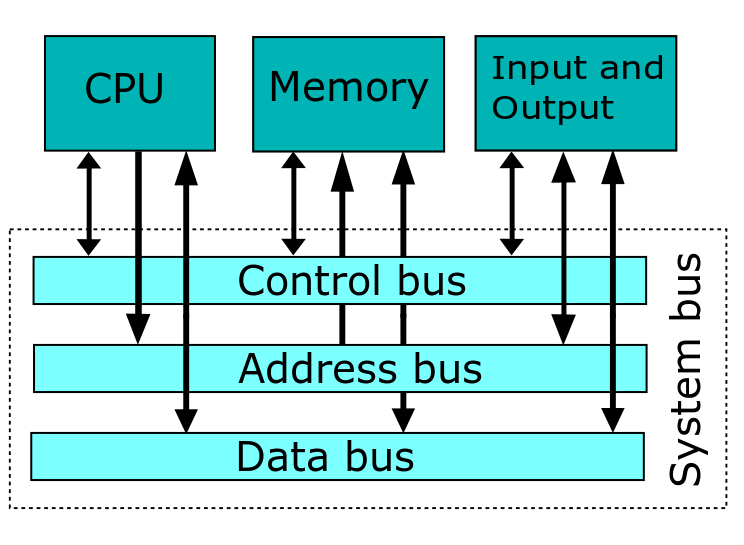
\includegraphics[width=\linewidth/2]{computer_system_bus}
  \caption{Magistrala systemowa \cite{image:system_bus}}
\end{center}
\label{fig:system_bus}
\end{figure}
% src: wiki

Mimo, że nowoczesne systemy komputerowe pod względem organizacji sprzętu wyglądają dużo bardziej
skomplikowanie, to model ten dobrze się sprawdza jako reprezentacja sprzętu dla
programisty systemu operacyjnego nie zajmującego się sterownikami urządzeń.

Poza podstawowym przesyłaniem danych większość magistral pozwala urządzeniom
zgłaszać przerwania [\ref{def:przerwania}], oraz dopuszcza możliwość transferu danych za pomocą DMA [\ref{sec:dma}].


\section{Mostki} % JM
W nowoczesnych systemach komputerowych istnieje wiele podłączonych do
siebie magistral z różnymi protokołami. Potrzebujemy w takim wypadku
mechanizmu, który pozwoli tłumaczyć protokół jednej szyny na drugi. Z
pomocą przychodzą układy zwane \textbf{mostkami} \cite{book:tanenbaum_hardware}. Możemy chcieć
tłumaczyć protokół magistrali ISA na PCI, bądź nawet PCI na PCI kiedy
magistrala PCI jest podłączona do innej magistrali
PCI. Standardowo w systemie występuje jedna magistrala PCI i jak każda magistrala tego typu
ma ona limit urządzeń. Aby móc ich podłączyć więcej, rozwiązaniem jest właśnie mostek
typu PCI-PCI. 


\begin{figure}
  \begin{center}
    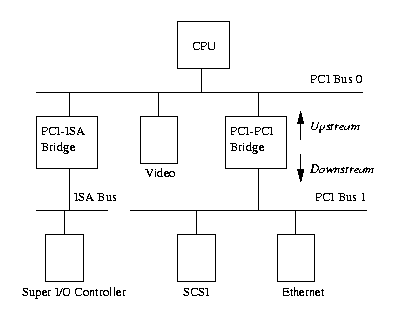
\includegraphics[width=\linewidth]{pci-system}
    \caption{Mostki i magistrale \cite{image:mostki}}
\end{center}
\end{figure}


\section{Organizacja systemu komputerowego} % JM
% https://en.wikipedia.org/wiki/Bus_(computing)
% Tanenbaum

Na przestrzeni lat, używano wielu różnych sposobów połączenia
komponentów komputera. Jednym z podstawowych jest wymieniona
wcześniej \ref{system_bus} koncepcja jednej szyny systemowej \cite{wiki:bus}.

W miarę jak procesory i pamięci stawały się coraz szybsze, zdolność jednej magistrali
do obsługi całego ruchu stawała się ograniczona. Z natury niezbyt szybkie urządzenia
wejścia-wyjścia dzieliły jeden kanał komunikacji z szybkimi i kluczowymi dla systemu urządzeniami.
Pojawiły się więc inne warianty organizacji komponentów w systemie \cite{book:tanenbaum_hardware}.


W przypadku procesorów firmy Intel magistrala najbliżej procesora 
nosi nazwę \textit{Front Side Bus} \cite{fsb}. Intel ostatecznie upublicznił
informację o niej, stąd niektóre procesory AMD również posiadają takową.
W niektórych kontekstach nazwa ta jest również wykorzystywana jako 
nazewnictwo przyprocesorowych magistral niezależnie od producenta.
% https://en.wikipedia.org/wiki/Front-side_bus

% https://en.wikipedia.org/wiki/Southbridge_(computing)
% https://en.wikipedia.org/wiki/Northbridge_(computing)
% http://just2good.co.uk/chipset.php
Jedną z koncepcji, będącą do niedawna w powszechnym użyciu jest architektura 
\textbf{mostu północnego} \cite{northbridge}\cite{just2good} i 
\textbf{mostu południowego} \cite{southbridge}\cite{just2good}.
Została ona wprowadzona przez firmę Intel.

Rozdzielenie wynika z potrzeby jak najszybszej interakcji procesora z pamięcią
operacyjną jak i kartą graficzną. Na tej ścieżce komunikacji znajdował się most
północny, który do procesora podłączony był magistralą \textit{Front Side Bus}.
Dodatkowo do mostu północnego podłączony most południowy miał 
obsługiwać wszystkie akcje związane z wejściem i wyjściem. W tym wypadku nie jest wymagana tak duża 
przepustowość jak dla pamięci RAM czy GPU, ponieważ urządzenia IO z natury 
są wolne i nie pod nie optymalizuje się system komputerowy.

Początkowo mostki były ze sobą połączone magistralą PCI, jednakże z czasem 
połączenie to zastąpiono nowszymi: DMI (Direct Media Interface) - w przypadku 
Intela, oraz UMI (Unified Media Interface) w przypadku AMD.

% https://www.intel.com/content/dam/www/public/us/en/documents/white-papers/ia-introduction-basics-paper.pdf
% https://stackoverflow.com/questions/41543267/is-intel-quickpath-interconnect-qpi-used-by-processors-to-access-memory
% https://superuser.com/questions/692058/dmi-2-0-vs-8-0-gt-s-qpi
% https://www.what-is-my-computer.com/intel-qpi.html
% https://arstechnica.com/civis/viewtopic.php?p=1487668
% https://arstechnica.com/civis/viewtopic.php?f=8&t=40557


\begin{figure}
  \begin{center}
    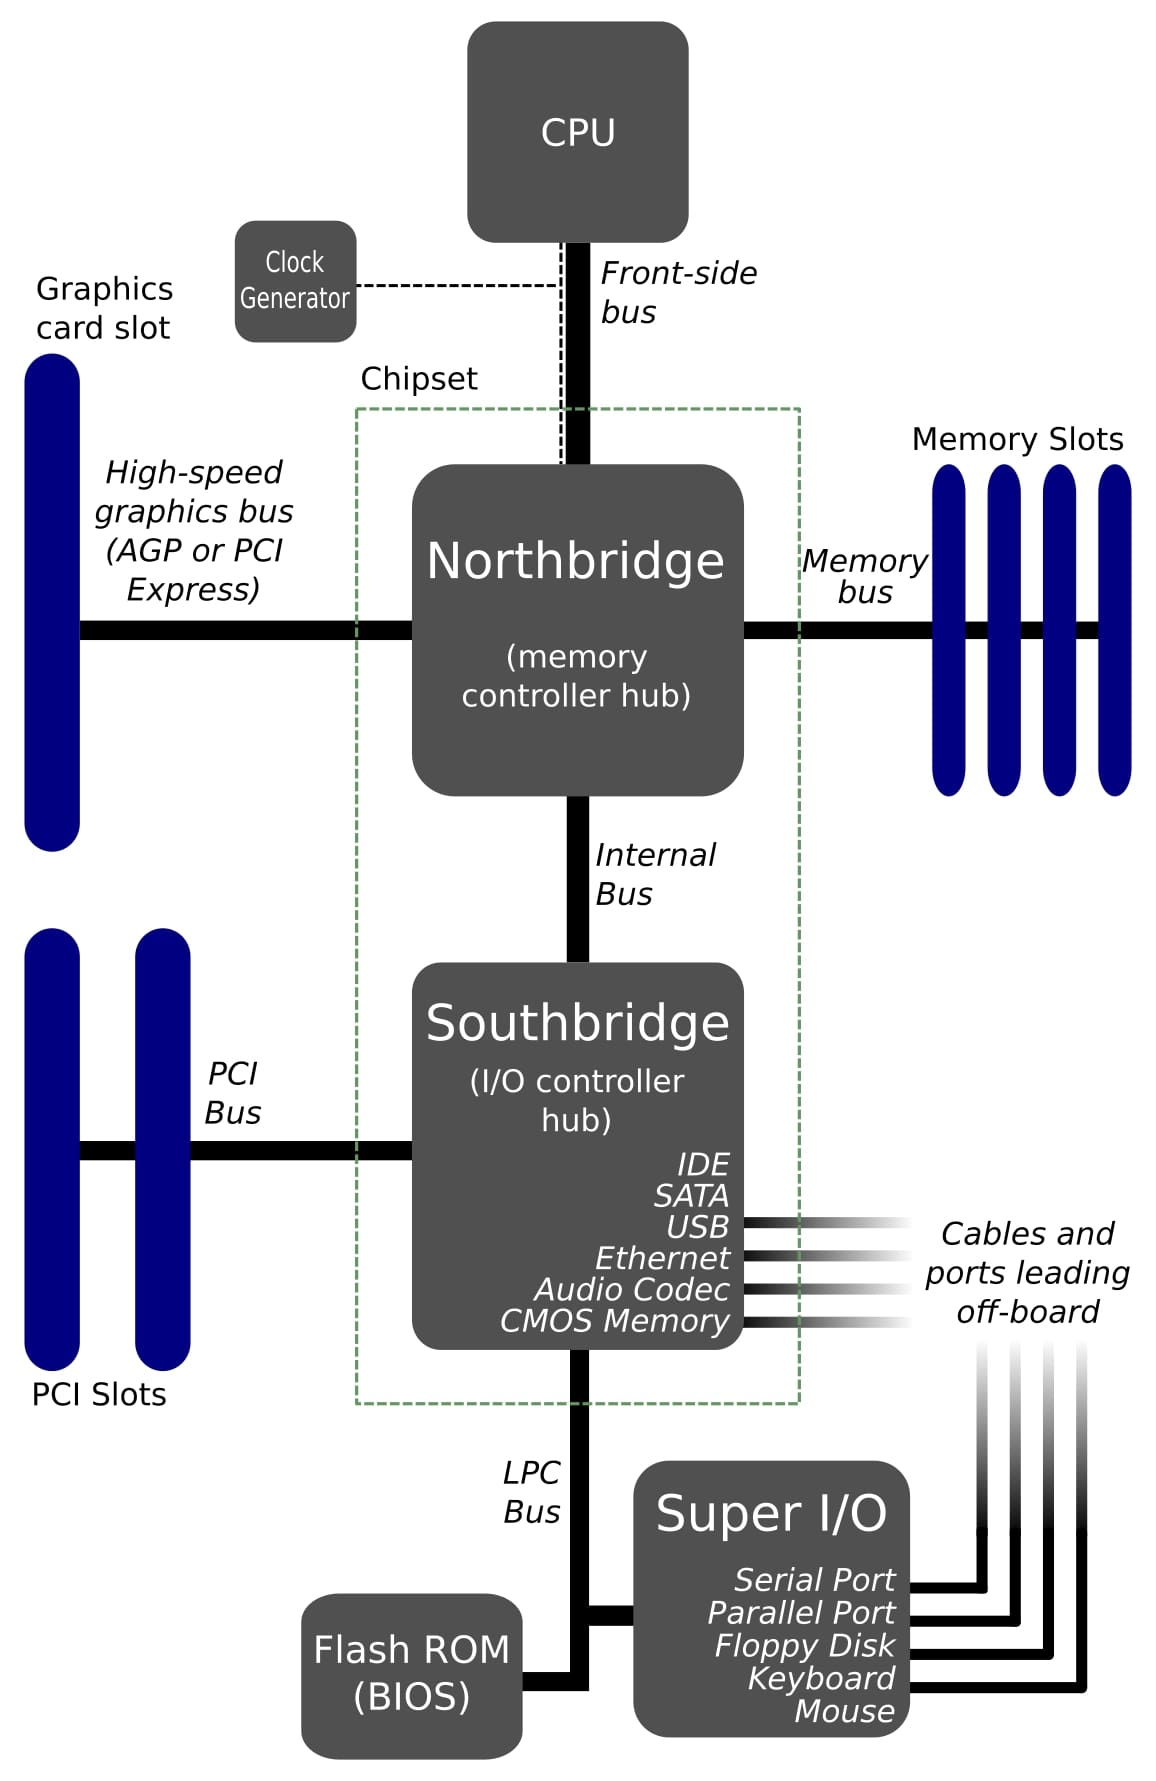
\includegraphics[width=\linewidth/2]{south_north_bridge}
  \caption{Architektura mostu północnego i południowego \cite{image:south_north_bridges}}
\end{center}
\end{figure}
% https://commons.wikimedia.org/wiki/File:Motherboard_diagram.svg

Przykładem systemu komputerowego opartego na
architekturze mostów północnego i południowego jest platforma Malta z
procesorem MIPS, pod którą działa system operacyjny Mimiker. Zostanie
ona omówiona w rozdziale \ref{sec:malta}.

Z czasem z powodów wydajnościowych kontrolery pamięci i GPU zostały
zintegrowane z procesorem, a funkcje mostu południowego przejął
\textbf{koncentrator PCH (ang. Platform Controller Hub)} używany w systemach komputerowych opartych o procesor 
architektury x86. Połączenie między CPU a PCH realizowane było przez DMI w kolejnej wersji.

\begin{figure}
  \begin{center}
    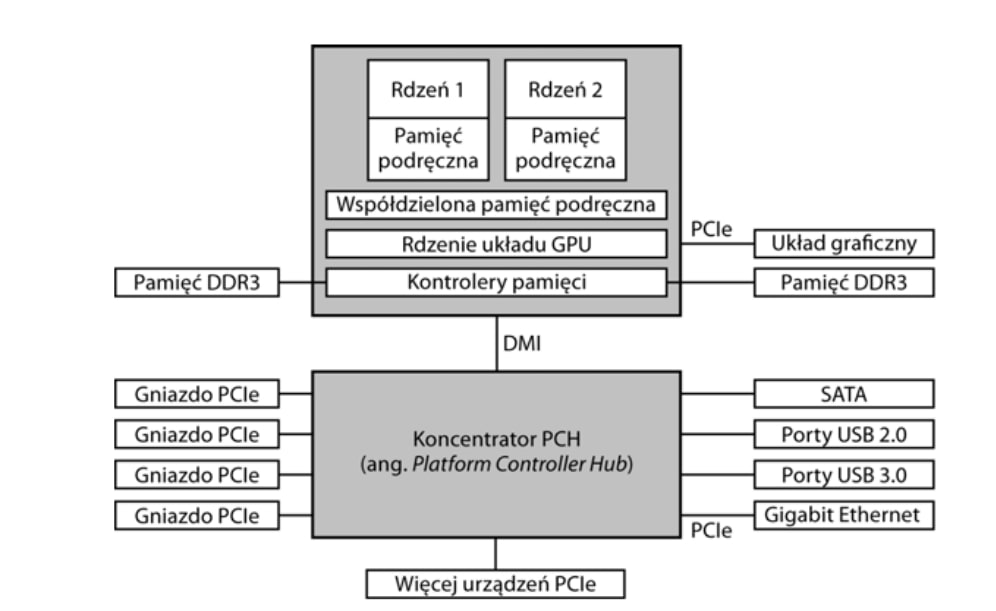
\includegraphics[width=\linewidth]{newer}
  \caption{System komputerowy oparty na procesorze architektury x86 z PCH \cite{image:pch}}
\end{center}
\end{figure}
% Tanenbaum, wydanie IV, rysunek 1.12


Obecnie dwie najnowsze architektury komunikacji komponentów
w systemie komputerowym to \textit{Quick Path Interconnect} \cite{quickpathinterconnect} firmy Intel
i \textit{Hypertransport} \cite{hypertransport} firmy AMD, które nie mieszczą się w zakresie
tej pracy. Są one sprzętowo zaimplementowane na płytach głównych. 
Głównie służą do łączenia wielu procesorów realizując między innymi protokoły spójności pamięci podręcznych \cite{cache_coherence}.
W dużym uproszczeniu bardziej przypominają sieć połączeń punkt-punkt \cite{wiki:point_point} z przesyłaniem
komunikatów, niż magistrale w standardowym rozumieniu.


\chapter{Sposoby komunikacji z urządzeniami i ich zasoby}

\section{Zasoby} % JM
\label{sec:zasoby}
% https://www.safaribooksonline.com/library/view/linux-device-drivers/0596000081/ch02s05.html
% http://haifux.org/lectures/323/haifux-devres.pdf
% http://fxr.watson.org/fxr/source/mips/include/resource.h?v=FREEBSD11

Sterowniki urządzeń oprócz standardowego, dynamicznego rezerwowania pamięci wymagają również rezerwacji
innego rodzaju zasobów \cite{zasoby2}. Najważniejszymi i najczęściej używanymi z nich są linie przerwań,  
zakresy portów wejścia-wyjścia, jak i zakresy pamięci używanej przez mechanizm MMIO, oraz kanały DMA 
\cite{book:linux_device_drivers}\cite{resource_h}.
Obecność tych zasobów wynika bezpośrednio ze sprzętowej organizacji systemu komputerowego jak i 
charakterystyki samego urządzenia. Urządzenia jak i kontrolery mogą udostępniać pamięć, posiadać zestaw rejestrów,
bądź reagować na przerwania czy obsługiwać transfery DMA.
Charakterystyka jak i sposoby użycia danych zasobów do komunikacji 
z systemem operacyjnym zostaną omówione w następnych sekcjach pracy, natomiast mechanizmy ich 
rezerwacji zostaną przedstawione na przykładzie systemu FreeBSD w rozdziale poświęconym temuż systemowi .

\section{Komunikacja} % WM

Każdą komunikację z urządzeniem jesteśmy w stanie uprościć do
wysyłania i odbierania danych, co czasem jest wspomagane przerwaniami.
Do głośnika będziemy wysyłali dane reprezentujące dźwięk, z mikrofonu będziemy je odbierali. 
Klawiatura po wciśnięciu przycisku informuję system za pomocą przerwania o nowych danych czekających na odczyt.

Najczęściej wyróżnia się trzy uzupełniające się wzajemnie rodzaje komunikacji. 
Najprostsze i nierzadko najlepsze jest regularne \textbf{odpytywanie (ang. pooling)} urządzenia.
Czasem jednak się nie jest to satysfakcjonujące rozwiązanie. Na przykład klawiatura bardzo rzadko 
(z punktu widzenia komputera) ma coś do zasygnalizowania. Ale kiedy zostanie wciśnięty przycisk, chcielibyśmy,
aby system operacyjny dowiedział się o tym jak najszybciej. Temu właśnie służą przerwania. Jest to sposób, w jaki 
urządzenie może samo zainicjować komunikację, a nie czekać na inicjatywę ze strony systemu operacyjnego. 
W celu zoptymalizowania obsługi transferów danych, wymyślono mechanizm \textbf{DMA - Direct Memory Access}, dzięki któremu
 procesor może zainicjować transfer danych, 
zająć się czymś innym, a kiedy dane będą gotowe, odczytać je z pamięci operacyjnej, 
co trwa znacznie krócej, niż odczyt bezpośrednio z dysku.


\section{PIO - Programowane wejście-wyjście} % WM
% http://inputoutput5822.weebly.com/programmed-io.html
% https://en.wikipedia.org/wiki/Memory-mapped_I/O

\textbf{Programowane wejście-wyjście} \cite{def:pio} jest zdecydowanie najprostszym mechanizmem IO. 
Procesor na polecenie sterownika inicjuje transfer danych z urządzeniem, następnie czeka na 
informację zwrotną. Niestety takie podejście jest uciążliwe, jeśli urządzenia i transfer 
danych są wolniejsze, niż sam procesor, co zazwyczaj ma miejsce. 

Istnieją dwa sposoby implementacji tego mechanizmu. Pierwszy z nich - 
\textbf{MMIO - ang. Memory Mapped IO - wejście-wyjście mapowane na pamięć} \cite{def:mmio} - polega na użyciu 
adresów z tej samej przestrzeni, dla pamięci operacyjnej oraz urządzeń. To sprawia, że 
interakcja z urządzeniami odbywa się za pomocą dokładnie tych samych instrukcji procesora, 
oraz w większości tej samej infrastruktury, co dostęp do pamięci. Urządzenia w tym przypadku są 
podłączone do tej samej szyny adresowej, co pamięć operacyjna.


Drugie podejście to \textbf{PMIO - ang. Port Mapped IO - wejście-wyjście mapowane na porty} -  
gdzie pamięć urządzeń znajduje się w odrębnej przestrzeni
adresowej. Jest to bardziej skomplikowany sposób implementacji PIO,
ponieważ wymaga dodatkowych instrukcji procesora, dlatego raczej nie
znajduje ono zastosowania w prostych procesorach RISC oraz w systemach
wbudowanych. Jeśli PMIO zostało zaimplementowane z użyciem odrębnej
fizycznej szyny adresowej, może to oznaczać zysk na wydajności.

PMIO nie zabiera adresów z fizycznej przestrzeni, co było dużą zaletą w przypadku 
16 i 32 bitowych procesorów. W układach 64-bitowych przestaje mieć to znaczenie. 
PMIO w zasadzie składa się z dwóch instrukcji - LOAD i STORE. Chcąc dokonać 
inkrementacji wartości w rejestrze urządzenia, musimy wykonać co najmniej trzy 
instrukcje - LOAD, INCREMENT, STORE. Przy MMIO można użyć każdej instrukcji 
która działa na pamięci, czyli na przykład w przypadku x86 wystarczy jedna instrukcja INC.


\section{Interrupt driven io} % WM
\label{def:przerwania}
% http://www.jonmasters.org/blog/2007/12/12/everything-you-know-about-interrupts-is-wrong/
% https://pdos.csail.mit.edu/6.828/2014/readings/hardware/8259A.pdf
% https://notes.shichao.io/lkd/ch7/
% https://en.wikipedia.org/wiki/Message_Signaled_Interrupts
% https://en.wikipedia.org/wiki/Advanced_Programmable_Interrupt_Controller


\textbf{Przerwania} są mechanizmem pozwalającym na zainicjowanie komunikacji przez urządzenie, a nie procesor. 
Jest to niezwykle ważne w przypadku urządzeń, które wymagają uwagi rzadko, ale natychmiast po 
wystąpieniu obsługiwanego przez nie zdarzenia.
Przykładem jest klawiatura, karta sieciowa i przycisk na obudowie. Regularne ich odpytywanie 
byłoby skrajnie nieopłacalne, ponieważ prawie zawsze okazywałoby się, że nie wymagają uwagi. 
Zbyt rzadkie odpytywanie z kolei sprawiałoby, że urządzenie byłoby mało responsywne.

Tradycyjnie, przerwanie było zgłaszane przez zmianę stanu na odpowiednim wyprowadzeniu 
procesora lub kontrolera przerwań. W momencie wykrycia przerwania przez procesor, przekazuje on sterowanie do odpowiedniej 
procedury systemu operacyjnego, której zadaniem jest zapisanie kontekstu aktualnie wykonywanego procesu, 
odnalezienie odpowiedniego sterownika i przekazanie kontroli zarejestrowanej przez niego procedurze obsługi przerwań. 
Następnie system operacyjny przywraca kontekst uprzednio wykonywanego procesu i oddaje mu sterowanie.

Procesor nie posiada osobnych wyprowadzeń do obsługi każdego urządzenia z
osobna. Zamiast tego, podłączało się do niego układy wspomagające nazywane \textbf{PIC
- ang. Programmable Interrupt Controller - Programowalny Kontroler Przerwań}. Tradycyjnie
 stosowano układ Intel 8259\cite{8259a}, który był w stanie
obsłużyć 8 linii przerwań (IRQ), samemu używając jednej. Nie było to wystarczająco,
więc dokładano drugi taki układ, podłączając go do portu nr 2 pierwszego. 
To dawało w sumie 15 wolnych linii przerwań i to przez długi czas wystarczało.


Większość linii było na stałe przypisanych do konkretnych urządzeń:

\begin{figure}
  \begin{center}
    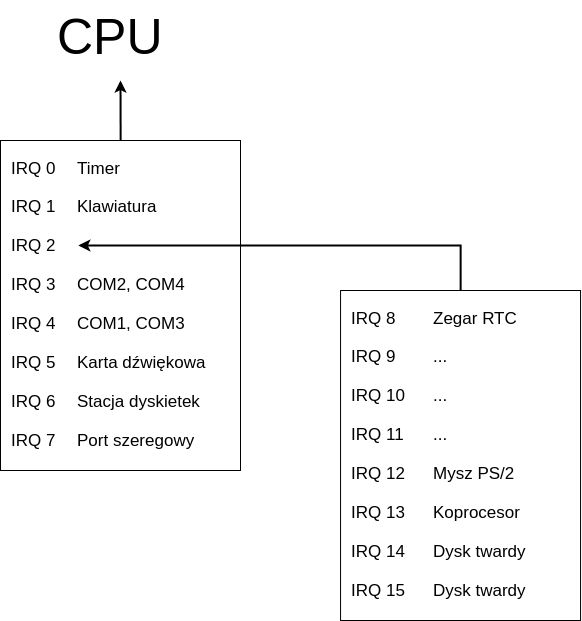
\includegraphics[width=\linewidth/2]{pic}
    \caption{Sposób połączenia dwóch układów Intel 8259}
  \end{center}
\end{figure}

Oczywiście powodowało to problemy. Autorzy listy nie mogli przewidzieć jaki
sprzęt powstanie w przyszłości. 

Układy PIC obsługują maski oraz priorytety. Dwa przerwania mogą nadejść
jednocześnie. W takim przypadku to o wyższym priorytecie zostanie przetworzone
pierwsze. 
Jeśli przerwanie nadejdzie w trakcie obsługi innego, zazwyczaj chcemy
wywłaszczyć poprzednie tylko jeśli ma ono niższy priorytet od nowego. 

Maski przerwań służą do wyłączenia konkretnych linii, co jest potrzebne na przykład,
gdy nie chcemy, aby w trakcie obsługi danego przerwania, nadeszło drugie
identyczne. Także przerwania muszą zostać wyłączone na czas wykonywania kodu,
który musi zostać wykonany atomowo, co w tym wypadku znaczy, że zmiana
kontekstu w trakcie jego wykonania mogłaby mieć złe skutki.
Przykładem tego jest zapisanie kontekstu wątku przy przełączeniu kontekstu.

W internecie nadal można znaleźć instrukcje typu “jak rozwiązać konflikt między
myszą podłączoną przez port COM 1 oraz modemem podłączonym przez port COM 3”. Oba te
urządzenia domyślnie używały linii IRQ4. Rozwiązać taki problem dało się na
wiele sposobów, na przykład przez konfigurację w biosie, fizyczną zmianę slotu,
do którego urządzenie jest podłączone lub przez przestawienie odpowiednich
zworek w sprzęcie. Podłączonych urządzeń było coraz więcej, więc zarządzanie
tym ręcznie byłoby problematyczne. Na szczęście powstały interfejsy z
automatyczną konfiguracją. 


Wraz z nadejściem procesorów wielordzeniowych, zwykły PIC przestał wystarczać. 
Z pomocą przyszedł \textbf{APIC - ang. Advanced Programmable Interrupt 
Controller}, który zasadniczo składa się z dwóch modułów. Pierwszym jest \textbf{Local 
APIC - LAPIC}, jeden dla każdego rdzenia procesora, często w niego fizycznie 
wbudowany. Każdy z nich obsługuje 255 linii przerwań.  
 
LAPIC mogą służyć także do przekazywania Między-Procesorowych przerwań (\textbf{IPI - 
Inter-Processor Interrupt}). W ten sposób rdzenie procesora są w stanie  komunikować się między sobą na przykład w celu 
nakazania innym procesorom wyczyszczenia TLB (TLB shootdown), lub pamięci podręcznej MMU, 
gdy stanie się ona nieważna.
 
Drugim modułem jest \textbf{I/O APIC}, zazwyczaj przypadający w jednym egzemplarzu na 
każdy kontroler magistrali. I/O APIC jest w stanie 
obsłużyć zazwyczaj 24 linie przerwań, a jako, że samych układów może być wiele, 
ilość linii przerwań nie stanowi już problemu. Każdy I/O apic trzyma w swojej 
pamięci informację, do którego LAPIC powinien przekazać które przerwanie. 

Wraz ze wzrostem zapotrzebowania na ilość linii przerwań oraz prędkość,  zaczęto
stosować Message Signalled Interrupts - \textbf{Przerwania Sygnalizowane Wiadomością - ang. Message Signaled Interrupts 
- MSI} \cite{def:msi}. Polega to na przesyłaniu krótkiej informacji opisującej przerwania poprzez główny
kanał komunikacji, zamiast stosowania osobnych ścieżek do obsługi przerwań. 
Najczęściej służy do tego MMIO.  Urządzenie chcąc wyzwolić przerwania, zapisuje 
jej opis pod ustalony adres, a docelowy APIC wyłapuje je i przekazuje do procesora.

PCI wspiera MSI od wersji 2.2. W PCI-Express jest to jedyny sposób dostarczania przerwań. 
MSI zwiększa liczbę obsługiwanych przerwań i znacząco upraszcza implementację sprzętu.
Dzieje się to kosztem utrudnienia projektowania urządzeń.  Współdzielenie szyny danych
z pamięcią może w niektórych przypadkach rozwiązać problem wyścigów między przerwaniem, a zapisem do pamięci
przez urządzenie. Nie potrzebna jest w takim wypadku dodatkowa synchronizacja, co oznacza
zysk na wydajności. 


Specjalnym rodzajem przerwań są przerwania synchroniczne. 
Nie są one wyzwalane
przez sprzęt, lecz są wynikiem działania programu, a więc działają
synchronicznie względem niego. Przykładem jest implementacja wywołań
systemowych w niektórych architekturach - odpowiednia
instrukcja powoduje przerwanie, które jest obsługiwane przez jądro, które
następnie określa jakie wywołanie systemowe miało miejsce. Innym przykładem są
wyjątki, takie jak dzielenie przez zero czy błąd stronicowania.



Specjalny plik /proc/interrupts pokazuje liczbę przerwań, które miały miejsce na każdej z linii.

\begin{lstlisting}[caption={Uproszczony plik /proc/interrupts \protect\footnotemark}]
      CPU0    CPU1        
 0:       9     0  IR-IO-APIC  2-edge       timer
 1:  219100     0  IR-IO-APIC  1-edge       i8042
 8:       0     1  IR-IO-APIC  8-edge       rtc0
 9:   11112    51  IR-IO-APIC  9-fasteoi    acpi
12: 1772765     0  IR-IO-APIC  12-edge      i8042
18:       0     0  IR-IO-APIC  18-fasteoi   i801_smbus
40:       0     0  DMAR-MSI    0-edge       dmar0
41:       0     0  DMAR-MSI    1-edge       dmar1
42:       0     0  IR-PCI-MSI  458752-edge  PCIe PME
43:       0     0  IR-PCI-MSI  464896-edge  PCIe PME
44:       0     0  IR-PCI-MSI  466944-edge  PCIe PME
45:       0     0  IR-PCI-MSI  49152-edge   snd_hda_intel:card0
46: 2941213     0  IR-PCI-MSI  512000-edge  ahci[0000:00:1f.2]
47:       0   448  IR-PCI-MSI  327680-edge  xhci_hcd
48:       0     0  IR-PCI-MSI  360448-edge  mei_me
49: 9885017     0  IR-PCI-MSI  32768-edge   i915
50: 9825069     0  IR-PCI-MSI  1048576-edge iwlwifi
51:     770    21  IR-PCI-MSI  1572864-edge nvkm
52:       0  4488  IR-PCI-MSI  442368-edge  snd_hda_intel:card1
(...) 
TLB: 776285 786805 TLB shootdowns
(...)
\end{lstlisting}
\footnotetext{Wydruk pochodzi z systemu \textit{Manjaro 17.1.11 Hakoila}, 
z jądrem w wersji \textit{x86\_64 Linux 4.17.12-1.1-MANJARO}, i procesorem
\textit{Intel Core i5-5200U @ 4x 2.7GHz}.}


Pierwsza kolumna to nazwa przerwania, zazwyczaj będąca numerem, który jest także jego priorytetem. 
Następnych kilka to liczba przerwań wygenerowanych na danym procesorze przez dane przerwanie. 
Wyraźnie widać, że większość z nich była kierowana do jednego lub dwóch procesorów.  
Reszta tabeli mówi o sposobie dostarczenia przerwania oraz nazwie urządzenia. 
System operacyjny stara się równomiernie rozłożyć przerwania na procesory. 
Da się to także zrobić ręcznie w łatwy sposób. 


 
\section{DMA - Direct Memory Access} % WM
\label{sec:dma}
% Tanenbaum
% https://en.wikipedia.org/wiki/Direct_memory_access
% http://www.shrubbery.net/solaris9ab/SUNWdev/DRIVER/p25.html
% http://www.ece.ubc.ca/~edc/379.jan99/lectures/lec13.pdf

Zarówno PIO, jak i przerwania nie są w stanie obsłużyć dużych transferów danych 
w optymalny sposób. Dla przykładu przy komunikacji ze stacją dysków CD, przerwania
same w sobie nie nadawałyby się w ogóle. Mogą one tylko wspomagać PIO, informując 
o gotowości urządzenia. PIO z kolei zablokowałoby procesor na cały czas odczytu, 
co jest marnotrawstwem możliwości procesora, ponieważ większość czasu spędziłby czekając
na dane. 


Z pomocą przychodzi moduł \textbf{DMA - ang. Direct Memory Access - bezpośredni dostęp do pamięci} \cite{def:wiki_dma}, 
czyli układ który wykonuje transfery między 
pamięcią i urządzeniami (także między dwoma miejscami w pamięci, lub między dwoma urządzeniami), bez 
ciągłego zaangażowania procesora, który w tym  przypadku odpowiada jedynie za odpowiednie zaprogramowanie DMA. 

Wyróżnia się dwa rodzaje transferów DMA - Third-party DMA i First-party DMA. 
Third-party DMA oznacza kontroler, który wykonuje zlecone przez procesor transfery. 
Taki kontroler DMA może być wielokanałowy, a więc prowadzić więcej niż jeden transfer na raz. 
First-party DMA z kolei pozwala urządzeniom na wykonywanie transferów do i z pamięci bez 
zaangażowania procesora. 


DMA zazwyczaj działa w jednym z dwóch trybów - Burst Mode - Trybie Wiązki, lub 
Cycle Stealing Mode - Trybie Podkradania Cykli. W pierwszym przypadku transfer odbywa się 
dużymi blokami, pomiędzy dwoma miejscami w pamięci lub urządzeniami, a magistrale 
które biorą udział w danym transferze są całkowicie temu dedykowane, to znaczy, 
że nawet procesor nie może z nich korzystać. W cycle stealing mode, kontroler DMA przesyła kilka 
bajtów pomiędzy urządzeniem a pamięcią, po czym oddaje szynę do użytku przez CPU. 
Procesor przetworzywszy dane, zwraca kontrolę układowi DMA, który dokonuje 
kolejnego transferu. Ten sposób jest co prawda wolniejszy, ale sprawia, że dane przetwarzane są na bieżąco.


\chapter{Omówienie wybranych magistral.}

\section{ISA} % JM
\label{sec:isa}
% footnote: https://www.freebsd.org/cgi/man.cgi?query=device.hints&sektion=5&manpath=freebsd-release-ports
% https://en.wikipedia.org/wiki/Industry_Standard_Architecture

Magistrala ISA \cite{def:wiki_isa} powstała jako magistrala systemowa [\ref{system_bus}] komputerów linii IBM PC w 1981 roku.
Zaprojektowana została z myślą o podłączaniu kart rozszerzeń do systemu komputerowego
z możliwością bus masteringu [\ref{def:bus_mastering}].

System operacyjny z urządzeniami peryferyjnymi podłączanymi pod magistralę ISA
musi mieć szczegółową wiedzę na temat podłączanego sprzętu i jego organizacji.
Oznacza to, że użytkownik systemu musi ręcznie konfigurować każde podłączane urządzenie,
czyli ustawić parametry takie jak linie przerwań, adresy portów IO, kanały DMA [\ref{sec:dma}][\ref{sec:zasoby}] 
\footnote{Na przykład w systemie FreeBSD takim mechanizmem jest \textit{device.hints} \cite{man:device.hints_5}}.


Tego rodzaju problemy spowodowały pojawienie się systemu ISA PnP (ISA Plug and Play \cite{def:wiki_legacy_pnp}),
który wprowadzał modyfikacje do sprzętu, BIOSu oraz systemu operacyjnego, które pozwalały
na automatyczną konfigurację urządzeń. Standard ten jednak nie przyjął się ponieważ
nie został wystarczająco szybko dopracowany, oraz mało urządzeń z niego korzystało.
Dodatkowo magistralę ISA zaczęła wypierać magistrala PCI [\ref{sec:pci}].

Obecnie większość nowoczesnych komputerów nie posiada fizycznej magistrali ISA,
jednak wszystkie systemu architektury x86 posiadają wirtualną magistralę ISA
przez którą wbudowane w płytę główną kontrolery mogą świadczyć proste 
usługi jak na przykład monitorowanie temperatury i napięcia podzespołów.

\section{Peripherial Component Interconnect - PCI} % JM
\label{sec:pci}

% https://wiki.osdev.org/PCI
% https://en.wikipedia.org/wiki/PCI_configuration_space
% https://en.wikipedia.org/wiki/Conventional_PCI

Nie będziemy omawiali magistrali PCI w całości, a skupimy się na
aspektach ważnych z punktu widzenia programisty systemu
operacyjnego. Omówimy między innymi sposób wykrywania urządzeń podłączonych do magistrali,
adresowanie urządzeń i alokację oferowanych przez nie zasobów pamięciowych.

Magistrala PCI pojawiła się jako następca
przestarzałej już magistrali ISA.  Służy ona w głównej mierze do
podłączania kart rozszerzeń do płyty głównej w komputerach PC. Poza tym 
może również łączyć kontrolery zintegrowane z płytą główną (np. most północny z
południowym).

Magistrala PCI posiada mechanizm \textbf{Plug and Play} \label{def:plug_and_play}\cite{def:wiki_plug_play}. 
Termin ten oznacza, że magistrala
daje możliwość detekcji i konfiguracji urządzeń do niej podłączonych bez wcześniejszej 
manualnej konfiguracji, bądź interwencji użytkownika. Wszelakie konflikty między 
urządzeniami również mogą być rozwiązane automatycznie.

System jest w stanie zidentyfikować podłączone urządzenie (w przypadku
PCI-express nawet podłączone w trakcie działania systemu
(ang. \textit{hot plug})), na podstawie numerów identyfikacyjnych, a
następnie odpowiednio dobrać sterownik.  Informacje o danym urządzeniu
zapisane są w ustandaryzowanej, znajdującej się na każdym urządzeniu PCI, przestrzeni 
zwanej \textbf{przestrzenią konfiguracyjną}. Jest to pamięć do której możemy zapisywać i czytać z niej.
Znajdziemy tam takie informację jak numer
producenta danego sprzętu (VID - Vendor ID), klasę urządzenia (Class
Code), oraz numer wewnętrznie nadany przez producenta pozwalający
zidentyfikować konkretny model urządzenia (DID - Device ID).

Pola Subsystem ID (SSID) i Subsystem Vendor ID (SVID) identyfikują konkretny model
urządzenia (np. karty rozszerzeń). VID identyfikuje producenta chipsetu, a SVID
producenta karty rozszerzeń na której znajduje się owy chipset. 
SSID wybierany jest z tej samej puli co DID. Jako przykład mogą posłużyć karty graficzne,
gdzie producentem chipsetu będzie nVidia, a producentem całej karty będzie Asus.

\begin{lstlisting}[caption={Część wydruku komendy lspci -v -nn \protect\footnotemark},label={lspci2}]
03:00.0 3D controller [0302]: NVIDIA Corporation GM108M 
[GeForce 840M] [10de:1341]
  Subsystem: ASUSTeK Computer Inc. GM108M [GeForce 840M] 
    [1043:12df]
  Flags: bus master, fast devsel, latency 0, IRQ 51
  Memory at f6000000 (32-bit, non-prefetchable) [size=16M]
  Memory at e0000000 (64-bit, prefetchable) [size=256M]
  Memory at f0000000 (64-bit, prefetchable) [size=32M]
  I/O ports at e000 [size=128]
  Expansion ROM at f7000000 [disabled] [size=512K]
  Capabilities: [60] Power Management version 3
  Capabilities: [68] MSI: Enable+ Count=1/1 Maskable
  Capabilities: [78] Express Endpoint, MSI 00
  Capabilities: [250] Latency Tolerance Reporting
  Capabilities: [258] L1 PM Substates
  Kernel driver in use: nouveau
  Kernel modules: nouveau
\end{lstlisting}
\footnotetext{Wydruk pochodzi z systemu \textit{Manjaro 17.1.11 Hakoila}, 
z jądrem w wersji \textit{x86\_64 Linux 4.17.12-1.1-MANJARO}, i procesorem
\textit{Intel Core i5-5200U @ 4x 2.7GHz}}

Na listingu \ref{lspci2} klasa (Class Code) urządzenia to \textit{3D controller} identyfikowana numerem
0x0302.
Producentem (VID) jest NVIDIA Corporation (0x10de), a samo urządzenie (DID) o nazwie GeForce 840M 
ma wewnętrznie nadany numer 0x1341.
SVID to ASUSTek Computer Inc. (0x1043) a SSID to Geforce 840M (0x12df).

Numery VID i SVID nadawane są przez organizację PCI-SIG \cite{pcisig}.
Na podstawie pary VID, DID, oraz Class Code, system operacyjny może automatycznie
dobrać odpowiedni sterownik. Korzystając z SVID i SSID system może sparować z urządzeniem
sterownik implementujący pewne dodatkowe funkcje wprowadzone przez producenta karty.

\begin{figure}
  \begin{center}
    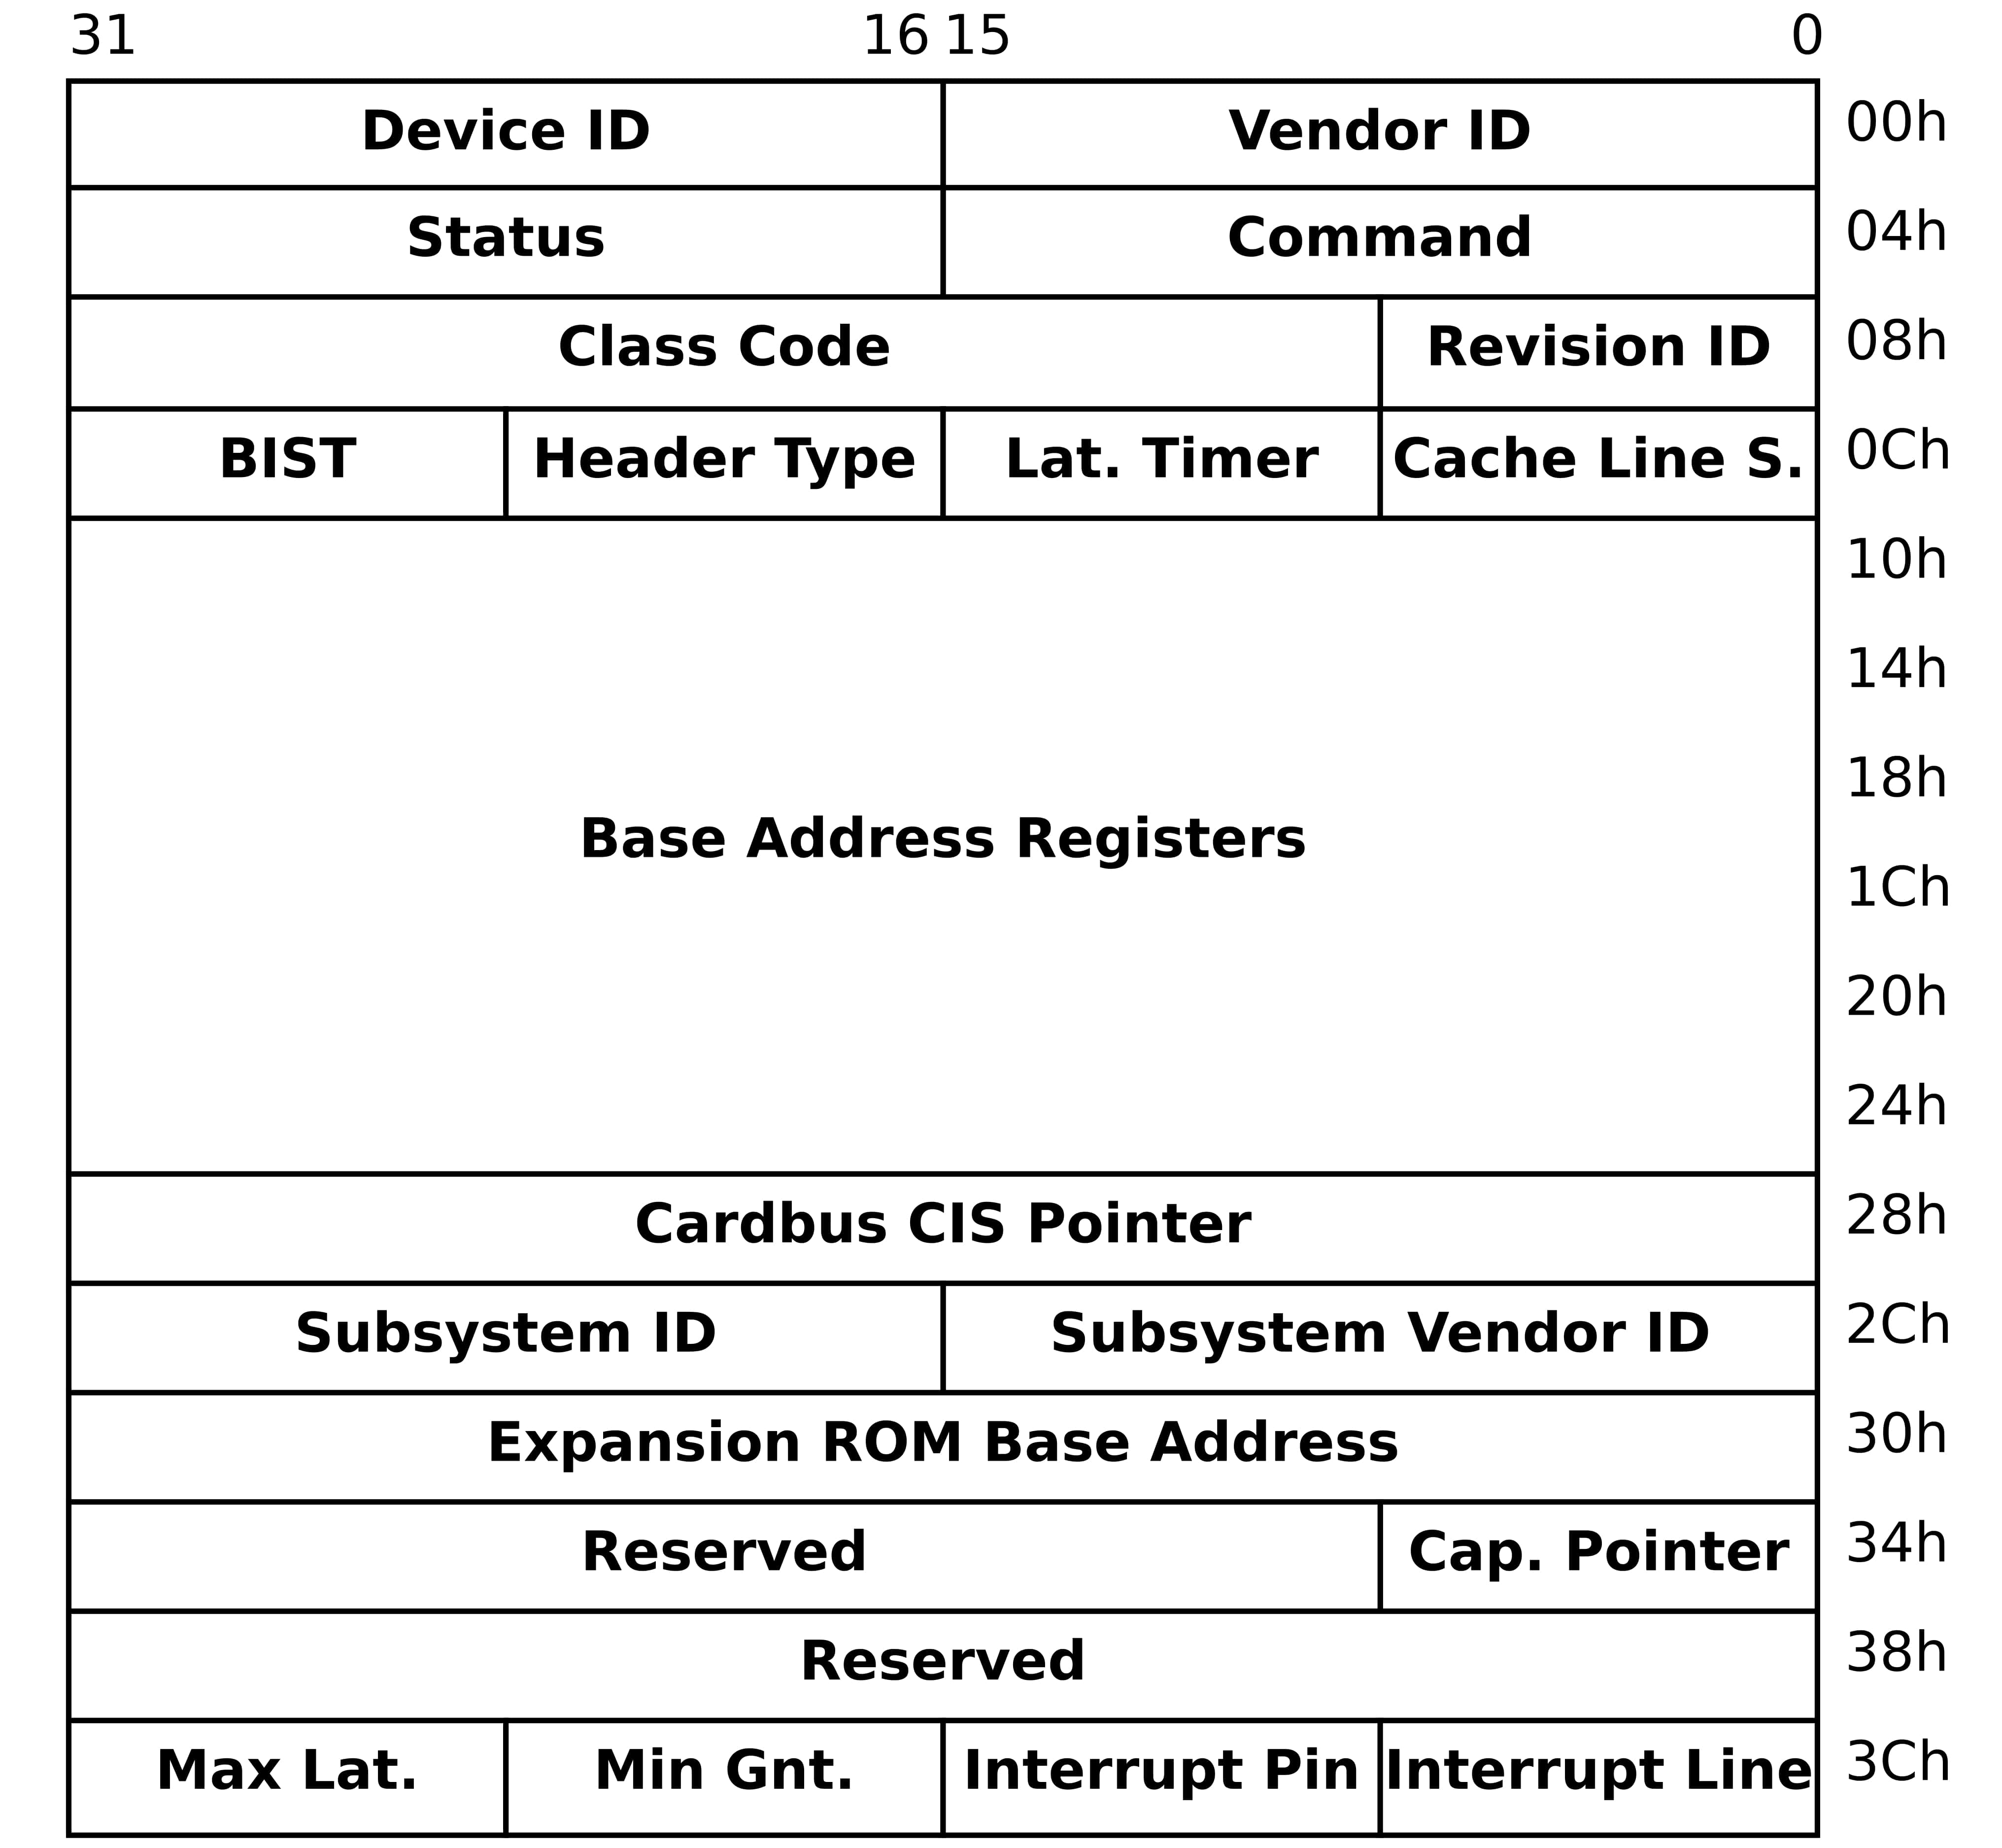
\includegraphics[width=\linewidth]{pci_config_space}
  \caption{Przestrzeń konfiguracyjna PCI \cite{image:pci_config_space}.}
\end{center}
\end{figure}
% src: wiki

Dostępy do przestrzeni konfiguracyjnej można wykonywać na dwa sposoby.
Pierwszy (\textit{legacy}), zwany \textit{Configuration Access Mechanism} pozwala na zapis i odczyt 
przestrzeni konfiguracyjnej przez porty IO o adresach 0xCF8 i 0xCFC. 
Ich symboliczne, zwyczajowe nazwy to \texttt{PCI\_CONFIG\_ADDRESS} i \texttt{PCI\_CONFIG\_DATA}.

Drugi mechanizm zwany \textit{Memory-Mapped Configuration} mapuje przestrzenie
konfiguracyjne urządzeń w fizyczną (a z pomocą systemu operacyjnego w wirtualną) przestrzeń adresową.
Dostępny jest w następcy standardowego PCI zwanym \textbf{PCI-express}.

Dostęp do portów \texttt{PCI\_CONFIG\_ADDRESS} i \texttt{PCI\_CONFIG\_DATA} jest możliwy, 
w zależnośći od architektury, poprzez 
instrukcje \texttt{in} i \texttt{out} jak na przykład w architekturze x86, 
albo rejestry te mogą być  dostępne poprzez adresowanie pamięci, tak jak 
na przykład na platformie Malta z procesorem MIPS.


Przy pisaniu bądź czytaniu z przestrzeni konfiguracyjnej w trybie \textit{legacy}, musimy wyspecyfikować 
magistralę PCI (możę być ich wiele w systemie), urządzenie i funkcję, oraz przesunięcie (ang. \textit{offset}) 
rejestru w przestrzeni konfiguracyjnej.

Poniżej wydruk komendy \texttt{lspci}. W pierwszej kolumnie znajdują się adresy
urządzeń PCI w formacie \texttt{MAGISTRALA:URZĄDZENIE:FUNKCJA}, zapisane szesnastkowo.
Pod jednym numerem urządzenia, może być wiele różnych funkcji danego urządzenia,
które mogą przez system być traktowane jako osobne byty
(tak jak w wypadku urządzenia o numerze 1c poniżej), bądź mogą to być różne urządzenia
zorganizowane w bardziej kompaktowy sposób (np. urządzenie o numerze 1f na listingu \ref{lspci1}).

\begin{lstlisting}[caption=Część wydruku komendy lspci \protect\footnotemark, label={lspci1}]
00:00.0 Host bridge: Intel Corporation Broadwell-U Host Bridge 
        -OPI (rev 09)
00:02.0 VGA compatible controller: Intel Corporation HD 
        Graphics 5500 (rev 09)
00:03.0 Audio device: Intel Corporation Broadwell-U Audio 
        Controller (rev 09)
00:14.0 USB controller: Intel Corporation Wildcat Point-LP USB 
        xHCI Controller (rev 03)
00:1b.0 Audio device: Intel Corporation Wildcat Point-LP High 
        Definition Audio Controller (rev 03)
00:1c.0 PCI bridge: Intel Corporation Wildcat Point-LP PCI 
        Express Root Port #1 (rev e3)
00:1f.0 ISA bridge: Intel Corporation Wildcat Point-LP LPC 
        Controller (rev 03)
00:1f.2 SATA controller: Intel Corporation Wildcat Point-LP 
        SATA Controller [AHCI Mode] (rev 03)
00:1f.3 SMBus: Intel Corporation Wildcat Point-LP SMBus 
        Controller (rev 03)
02:00.0 Network controller: Intel Corporation Wireless 7265 
        (rev 59)
03:00.0 3D controller: NVIDIA Corporation GM108M [GeForce 840M] 
        (rev a2)  
\end{lstlisting}
\footnotetext{Wydruk pochodzi z systemu \textit{Manjaro 17.1.11 Hakoila}, 
z jądrem w wersji \textit{x86\_64 Linux 4.17.12-1.1-MANJARO}, i procesorem
\textit{Intel Core i5-5200U @ 4x 2.7GHz}}

Odpowiednio zakodowany w słowie maszynowym adres zapisujemy w porcie \texttt{PCI\_CONFIG\_ADDRESS}.

\begin{lstlisting}[caption=Odczyt z przestrzeni konfiguracyjnej,escapechar=ß]
uint32_t pci_addr = 0x80000000 | bus << 16 | device << 11 
                    | function <<  8 | offset;
sysOutLong(PCI_CONFIG_ADDRESS, address);

return (uint16_t)((sysInLong (PCI_CONFIG_DATA) >> 
       ((offset & 2) * 8)) & 0xffff);
\end{lstlisting}

Przy dostępie do \texttt{PCI\_CONFIG\_DATA} wymagane jest ustawienie 31-szego bitu 
zwanego \textit{ECD (Enable Config Data)}.

Po odpowiednim zaadresowaniu, odczyt i zapis wykonujemy przez port \\
\texttt{PCI\_CONFIG\_DATA},
korzystając z instrukcji in i out, bądź w przypadku zmapowania tego rejestru w pamięć,
za pomocą zwykłych instrukcji operujących na pamięci.
W powyższym przykładzie zadanie to spełniają funkcje \texttt{sysOutLong} i \texttt{sysInLong}.

W przypadku zmapowanych w pamięć przestrzeni konfiguracyjnych, system operacyjny
powinien dla każdego potencjalnie podłączonego urządzenia zarezerwować 4 KiB miejsca. 
Przestrzenie konfiguracyjne dostępne są wtedy poprzez C-ową tablicę postaci
\texttt{config\_space[bus][device][function]}.
Daje to 256 możliwych wyborów magistrali, po 32 urządzenia, po 8 funkcji, gdzie
każda przestrzeń konfiguracyjna jest wielkości 4 KiB. Razem 256 MiB pamięci
potrzebnej na obsługę jednej magistrali PCIe.
Zatem na 32-bitowych systemach może dojść do sytuacji, gdzie fizycznie mamy 4 GiB pamięci RAM, ale 256 MiB
jest nieużywanych, ponieważ to miejsce zajmują przestrzenie konfiguracyjne urządzeń PCIe.

Następnymi ważnymi rejestrami w przestrzeni konfiguracyjnej są \textit{Base Address Registers (w skrócie BAR)}.
Jeśli urządzenie dysponuje zasobami pamięciowymi, to w BAR zakodowane są informacje
mówiące ile pamięci udostępnia urządzenie, oraz jak wykonywać do niej dostępy z
poziomu systemu.

BAR dzielą się na 2 rodzaje ze względu na sposób w jaki można wykonywać dostępy do
udostępnianego przez urządzenie zasobu.
Istnieją BAR typu \texttt{MEMORY} i typu \texttt{IO PORT}. Zasoby pierwszego typu
muszą być odwzorowane w fizyczną przestrzeń adresową odpowiadającą pamięci RAM,
natomiast zasoby drugiego typu przechowujące adres portu, mogą przechowywać dowolny adres
przestrzeni portów IO. Dostęp do odpowiadających nim przestrzeni wykonuje się kolejno za 
pomocą mechanizmów MMIO i PMIO.

% https://en.wikipedia.org/wiki/PCI_configuration_space#Bus_enumeration
Przy pierwszej interakcji z urządzeniem w BAR zakodowana jest wielkość zasobu pamięciowego,
jego typ, jak i flagi. Tabelki \ref{tab:memorybar} i \ref{tab:iobar} prezentują kodowanie początkowych informacji w BAR.

% https://wiki.osdev.org/PCI
\begin{table}
\begin{center}
\caption{Kodowanie informacji w BAR typu MEMORY}
\label{tab:memorybar}
\begin{tabular}{|c|c|c|c|}
\hline
\textbf{31-4} & \textbf{3} & \textbf{2-1} & \textbf{0}  \\ \hline
wyrównany do 16 bajtów adres bazowy & bit prefetchable & typ\tablefootnote{\url{https://wiki.osdev.org/PCI\#Base\_Address\_Registers}} & zawsze 0 \\
\hline
\end{tabular}
\end{center}
\end{table}

\begin{table}
\begin{center}
\caption{Kodowanie informacji w BAR typu IO}
\label{tab:iobar}
\begin{tabular}{|c|c|c|}
\hline
\textbf{31-2} & \textbf{1} & \textbf{0}  \\ \hline
wyrównany do 4 bajtów adres bazowy & zarezerwowane & zawsze 1 \\
\hline
\end{tabular}
\end{center}
\end{table}


System czytając wszystkie możliwe przestrzenie konfiguracyjne jest w stanie 
zidentyfikować wszystkie podłączone urządzenia. Po ich zidentyfikowaniu czyta rejestry BAR
każdego z urządzeń, dekodując zawarte w nich informacje. 
Dla każdego BAR po zarezerwowaniu odpowiedniej ilości miejsca w przestrzeni adresowej,
bądź w przestrzeni IO, w zależności od typu BAR, system wpisuje 
pierwszy adres zarezerwowanej przestrzeni do rejestru BAR.

% https://wiki.osdev.org/PCI#Base_Address_Registers


\section{USB} % WM
\label{sec:usb}
% https://www.beyondlogic.org/usbnutshell/usb1.shtml
% https://en.wikipedia.org/wiki/USB_(Communications)
% FreeBSD device drivers - chapter 15


Najpopularniejszym w dzisiejszych czasach standardem podłączania urządzeń
zewnętrznych jest \textbf{USB - Universal Serial Bus - Uniwersalna Magistrala
Szeregowa}. Tym samym złączem możemy podłączyć drukarkę, kamerę, dysk
zewnętrzny i klawiaturę. Występuje w kilku rozmiarach - standardowe montowane
w komputerach A, czasem spotykane w drukarkach B, dawniej popularne mini USB A i
B, bardzo częste w telefonach Micro, oraz zdobywające coraz większą
popularność USB - C. 

Standard mówi, że istnieje dokładnie jeden kontroler nadrzędny - master [\ref{def:master/slave}]. 
Tylko on może inicjować komunikację (a więc nie ma tu typowych linii przerwań). 

Pozostałe urządzenie są albo bezpośrednio
podłączone do niego, albo przez huby, zwane też koncentratorami. Tworzy to
topologię drzewa. Urządzenia są adresowane za pomocą 7 - bitowego identyfikatora, 
z czego 0 jest zarezerwowane. Zatem teoretycznie jeden
kontroler może obsłużyć do 127 urządzeń. Jednak jednak pozwala on na 
przepustowość wynoszącą maksymalnie 480 Mbit/s w standardzie 2.0, dlatego
czasem stosuje się więcej niż jeden.

Każde urządzenie USB może zarejestrować do 32 kanałów logicznych - 16 wejścia i 16 wyjścia.
Dzięki nim, jedno fizyczne urządzenie może obsługiwać więcej,
niż jedną funkcję, na przykład kamera internetowa może mieć osobne
kanały dla mikrofonu, kamery oraz przycisków sterowania. Mogą one
transmitować dane krótkimi wiadomościami, lub potokami. Są trzy tryby
potoków: izochroniczny, masowy (bulk) oraz przerwania.

Tryb izochroniczny gwarantuje minimalną przepustowość, ale nie
gwarantuje poprawnej transmisji. Ma on zastosowanie na przykład przy
komunikacji z mikrofonem. Tryb masowy (bulk) - gwarantuje poprawny
transfer, ale nie minimalną przepustowość, która jest zależna od
innych transferów.  Przykładem zastosowania jest pamięć masowa. Tryb
przerwaniowy gwarantuje minimalną częstotliwość
próbkowania. 

Warto zauważyć, że przerwania są tu zaimplementowane z
użyciem bardzo częstego próbkowania, ale dokonywanego przez
kontroler a nie przez procesor i sterownik urządzenia, dzięki czemu
nie ma to wpływu na wydajność reszty systemu. Tryb przerwaniowy jest
używany w urządzeniach takich jak mysz i klawiatura.

Standard USB został zaprojektowany z myślą o Plug and Play oraz hot plug. 
Urządzenia USB możemy podłączyć lub odłączyć z działającego komputera
w dowolnym momencie. Wyjątkiem są nośniki pamięci, do
których zapis może być wspomagany pamięcią podręczną, w takim wypadku należy
najpierw dane zsynchronizować (polecenie \textbf{sync} w linuksie). 

Sterownik jest
wybierany automatycznie przez system na podstawie informacji dostarczonych przez
urządzenie - VID, PID, klasa urządzenia. Numer VID jest nadawany producentowi
przez organizację standaryzacyjną. 

Standard stał się niezwykle popularny dzięki swojej prostocie. Przewód w najpopularniejszym 
standardzie 2.0, zawiera tylko dwie linie
przenoszące dane. Prostota protokołu ułatwia implementację w urządzeniach.
Dzięki klasom urządzeń, producent sprzętu nie musi zazwyczaj dostarczać
sterownika.

Informacje na temat urządzeń można zobaczyć używając polecenia \textit{lsusb -v} w systemie linux.


\chapter{Urządzenia i sterowniki w systemach operacyjnych}

\section{Sterowniki jako moduły jądra} % JM

W przypadku architektury mikrojądra sterownik może być specjalnym programem przestrzeni
użytkownika. W systemach uniksowych kod sterowników urządzeń wykonuje się zazwyczaj 
z uprawnieniami jądra ze względu na monolityczną architekturę.
Nie chcielibyśmy jednak ponownie kompilować
jądra za każdym razem gdy dodajemy nowy sterownik. Dodatkowo
posiadany system komputerowy w zasadzie nigdy nie korzysta ze
wszystkich dostępnych sterowników.
Z tych powodów, w większości systemów, sterowniki ładowane są do systemu
dynamicznie jako tzw \textbf{moduły jądra}.  Nazywane w środowisku
linuxowym LKM od \textit{Loadable Kernel Module} i KLD w środowisku
BSD \cite{wiki:lkm}.

Moduły jądra to dowolny kod, który może być załadowany do jądra w
dynamiczny sposób, czyli nawet podczas pracy systemu. Dodanie kodu w taki sposób
nie wymaga ponownej kompilacji reszty kodu.
Moduł jądra może również zostać odczepiony zwialniając zaalokowane wcześniej zasoby. 
Aby osiągnąć taki efekt
moduły jądra muszą implementować interfejs, który został zadany przez
jądro systemu. Kod modułu jądra, niezależnie od systemu operacyjnego,
musi najczęściej wyspecyfikować co najmniej procedurę reagującą na
zdarzenia związane z modułem takie jak jego załadowanie i
odczepienie, oraz zdefiniować strukturę opisującą ten moduł, która
będzie przeczytana przez system operacyjny i umożliwi załadowanie
modułu. W systemach opartych na jądrze Linux, moduły jądra mają strukturę 
bibliotek dzielonych, a jądro implementuje konsolidator dynamiczny.

Minusem modułów jądra może być ich użycie przez złośliwe oprogramowanie (tzw. rootkity \cite{rootkits}). 

Z tego powodu systemy wymagające wysokiego poziomu 
bezpieczeństwa mogą mieć systemy operacyjne skompilowane statycznie, z wyłączoną 
możliwością ładowania modułów.
Drugim minusem może być drobny narzut czasowy związany z obsługą modułów.
Dodatkowo, kod modułu po załadowaniu zazwyczaj nie zajmuje z kodem jądra ciągłego
zakresu adresów - występuje fragmentacja. Przez to wykonywanie kodu może wykorzystywać więcej wpisów TLB \cite{wiki:lkm}.

W niektórych systemach operacyjnych np. przeznaczonych na mniejsze urządzenia (IOT, wbudowane, RTOS),
czy w przypadku niektórych systemów o architekturze mikrojądra
wybór składowych części jądra jest możliwy tylko podczas kompilacji. Statycznie skompilowane jądro
pozwala pominąć całą skomplikowaną logikę odpowiadającą za zarządzanie modułami jądra.

Jak oprogramowanie klienckie korzysta z funkcjonalności sterownika?
Wiele systemów operacyjnych stosuje filozofię pochodzącą z systemów z rodziny Unix,
polegającą na reprezentowaniu urządzeń za pomocą plików. 
Za wywołaniami systemowymi dotyczącymi plików stoją różne semantyki w zależności od tego
czy mamy do czynienia ze standardowym plikiem dyskowym będącym ciągiem bajtów, czy może ze
specjalnym typem np. urządzeniem.

W przypadku pliku reprezentującego urządzenie, jego sterownik może implementować w 
zasadzie dowolne zachowanie dla każdego odnoszącego się do niego plikowego wywołania systemowego.

Między innymi w taki sposób jak wyżej opisany jądra udostępnia kod użytkownikowi, 
jednak samo jądro może taki kod wykorzystywać w dowolny sposób wołając funkcje 
zarejestrowane przez moduł jądra pod wyspecyfikowanym interfejsem.

Moduł jądra może również utworzyć \textbf{pseudourządzenia}.
Są to pliki logicznie będące urządzeniem w systemie, ale nie odpowiadające 
żadnemu urządzeniu fizycznemu.
Takie urządzenia w systemie GNU/Linux znajdują się zwyczajowo w katalogu /dev.
Są to takie urządzenia jak: \texttt{urandom}, \texttt{tty0}, \texttt{zero} czy \texttt{null}.

\section{Struktura kodu sterownika} % JM
% same src as in \label{sec:synchro}

% bounded sleep - blocking
% unbounded sleep - sleeping
% volountary context switching - sleep()

Wywołania procedur zdefiniowanych w sterowniku wynikają z różnych zdarzeń.
Procedury, których wywołanie wynika z jakiegoś żądania systemu operacyjnego 
(np. wywołania systemowego) względem sterownika, nazywamy
\textbf{górną połówką (ang. top half) \footnote{Posługujemy się tutaj nomenklaturą FreeBSD.
W przypadku jądra Linux nazewnictwo jest odwrotne.}}.
Wykonują się one synchronicznie w kontekście wątku jądra oczekującego na obsługę żądania IO i mogą
\textbf{spać}, czyli dobrowolnie oddać sterowanie.
% msleep(9) & bus_setup_intr(9)
% https://www.freebsd.org/cgi/man.cgi?query=bus_setup_intr&apropos=0&sektion=0&manpath=FreeBSD+8.1-RELEASE&format=html
% https://www.freebsd.org/cgi/man.cgi?query=msleep&apropos=0&sektion=9&manpath=FreeBSD+11-current&format=html
Najczęściej jest to konsekwencją próby zajęcia zajętej już blokady, bądź czekania
na zmiennej warunkowej.

Drugi zestaw procedur zwanych \textbf{dolną połówką (ang. bottom half)} to procedury
obsługi przerwań (ang. Interrupt Service Routines - ISR) pochodzących od urządzeń.
Z natury są asynchroniczne, stąd nie mogą zależeć od stanu konkretnego procesu. 
Przyjmijmy, że kod dolnej połówki wykonuje w kontekście przerwanego wątku, oraz
z wyłączonymi przerwaniami\footnote{Jest to uproszczenie. Systemy operacyjne stosują
bardzo różne mechanizmy do obsługi przerwań. Przypadek FreeBSD zostanie opisany
w rozdziale \ref{sec:synchro}}.

Z tego powodu dolną połówkę należy jak najszybciej opuścić, aby nie dopuścić
do niepożądanych zdarzeń. Gdyby wykonanie dolnej połówki trwało zbyt długo,
obsługa przerwań zagłodziłaby inne wątki.
W przypadku jeszcze dłuższego wykonania
mogłyby pojawić się efekty takie jak np. gubienie przerwań, które
z reguły całkowicie uniemożliwiają stabilną pracę systemu.
Tym bardziej kod dolnej połówki nie może spać, zatem jedynym
dozwolonym środkiem synchronizacji w takim wypadku będzie blokada wirująca.

Kolejnym zestawem funkcji są procedury odpowiadające za inicjalizację i konfigurację 
urządzenia, oraz reagowanie na akcje takie jak, wyłączenie, uśpienie, czy wybudzenie urządzenia.
W systemie FreeBSD są one używane przede wszystkim przez podsystem NewBus podczas 
procesu zwanego \textbf{autokonfiguracją}.

\section{Drzewo urządzeń} % JM

W dużej części systemów operacyjnych programowa reprezentacja urządzeń wynika 
z ich organizacji w sprzęcie - przypomina drzewo.

W systemie GNU/Linux polecenie \textit{lshw} pozwala wyświetlić owe drzewo.
Prezentujemy jednak przykład drzewa urządzeń w systemie FreeBSD ze względu na
jego wykorzystanie w dalszych rozdziałach.

\begin{lstlisting}[caption={Przykładowe drzewo urządzeń w systemie FreeBSD \cite{freebsd_book:tree}}, label={listing:device_tree}]
root0
  description: System root bus
  devclass: root, drivers: nexus
  children: nexus0

nexus0
    devclass: nexus, drivers: acpi, legacy, npx
    children: np0, legacy0

  legacy0
      description: legacy system
      devclass: legacy, drivers, eisa, isa, pcib
      children: eisa0, pcib0

    pcib0 /* southbridge */
        description: Intel 82443BX (440 BX) host to PCI bridge
        devclass: pcib, drivers: pci
        children: pci0
    pcib1
        description: PCI-PCI bridge
        devclass: pcib, drivers: pci
        children: pci1

      pci0
          description: PCI bus
          devclass: pci, drivers: ahc, eisab, atapci, xl ...
          children: agp0, pcib1, isab0, atapci0, ahc0, xl0

        atapci0
            description: Intel 82371AB PIIX4 IDE controller
            devclass: atapci, drivers: atadisk, atapicd
            children: atadisk0, atadisk1
            class: mass storage, subclass: ATA
            I/O ports: 0xffa0-0xffaf

          atadisk0
              devclass: atadisk, drivers: none
              interrupt request lines: 0xe
              I/O ports: 0x1f0-0x1f7, 0x3f6
          atadisk1
              devclass: atadisk, drivers: none
              interrupt request lines: 0xf
              I/O ports: 0x170-0x177, 0376
\end{lstlisting}

W korzeniu drzewa zazwyczaj znajduje się logiczne urządzenie nazywane rootdev bądź nexus.
Wszystkie inne urządzenia są jego potomkami. W liściach często znajdują się
fizyczne urządzenia, a na węzłach reprezentacja mostków, magistral i kontrolerów.

Widoczne są również zarezerwowane zasoby takie jak zakresy portów wejścia-wyjścia, czy przerwania.

\section{Urządzenia znakowe i blokowe} % JM
% https://www.freebsd.org/doc/en/books/arch-handbook/driverbasics-block.html
% https://www.freebsd.org/doc/en/books/arch-handbook/driverbasics-char.html
% https://jyotisingh92.wordpress.com/2017/12/23/block-driver-vs-character-driver/
% FreeBSD device drivers
% design and implementation of freebsd operating system

Różne typy urządzeń inaczej obsługują transfer danych z, i do urządzenia.
Urządzenia pozwalające na swobodny dostęp (ang. random access) do bloków danych 
stałej wielkości nazywamy \textbf{urządzeniami blokowymi}. Są to na przykład dyski 
twarde. 
\textbf{Urządzenia znakowe} charakteryzują się strumieniowym przesyłaniem danych i
nie pozwalają na swobodny dostęp. Tego typu urządzeniem jest na przykład karta dźwiękowa.

Naturalnie sterowniki różnych typów urządzeń będą się różnić. Można wtedy takie sterowniki
nazywać odpowiednio sterownikami blokowymi bądź znakowymi. Jednakże nazwy te nie 
zawsze są ściśle związane z typem obsługiwanego urządzenia, a raczej z interfejsem wystawianym
przez sterownik do systemu operacyjnego i użytkownika, stąd pojawiające się nazwy
\textbf{interfejs znakowy sterownika}, oraz \textbf{interfejs blokowy sterownika}.

Sterowniki blokowe przyjmują zlecenia zapisu bądź odczytu bloków. Zlecenia te, oraz dane
są buforowane i keszowane przez jądro systemu operacyjnego. Proces ten wymaga 
bardzo dużej i skomplikowanej logiki w systemie.

Interakcja ze sterownikami znakowymi korzysta z tego samego interfejsu co operacje 
na zwykłych plikach. W przypadku systemów POSIX można czytać i pisać za pomocą procedur 
\texttt{read()} i \texttt{write()}. Operacje te nie wymagają buforowania ani keszowania,
a ich obsługa jest znacznie prostsza.

W systemie operacyjnym FreeBSD blokowy interfejs do sterowników jest wycofywany z użycia oraz 
wysoce niezalecany w żadnym przypadku.
Głównym powodem jest niedeterminizm wykonania zlecanych operacji. Mianowicie, ze względu na
buforowanie i keszowanie zlecanych operacji zapisów, rzeczywiste zapisy mogły być
wykonane w innej kolejności niż zostały zlecone. Uniemożliwia to przewidzenie 
stanu dysku w dowolnym momencie czasu, co dalej czyni prawie niemożliwym 
analizę i naprawę zniszczonych struktur danych na dysku (np. systemów plików).

Dodatkowo rzeczywiste zapisy nie są wykonywane od razu. Powoduje to, że w przypadku
błędu, system operacyjny nie jest w stanie stwierdzić która ze zleconych operacji zawiniła.

We FreeBSD interfejs znakowy dla urządzeń dyskowych nazywany jest 
\textbf{surowym interfejsem (ang. raw-device interface)}.
 
\section{Start systemu} % JM
\label{sec:start_systemu}
% https://www.freebsd.org/doc/handbook/boot.html
% https://www.freebsd.org/cgi/man.cgi?query=boot&sektion=8

% https://www.cs.rutgers.edu/~pxk/416/notes/02-boot.html
% https://en.wikipedia.org/wiki/Booting

Przy starcie komputera, wstępna konfiguracja urządzeń dokonywana jest przez
oprogramowanie zapisane w nieulotnej pamięci na płycie głównej, 
czyli tzw. \textbf{firmware}. Jest ono zależne od płyty głównej i architektury procesora. 
Przykładami może być BIOS \cite{wiki:bios} i wypierające go UEFI \cite{uefi} w architekturze x86. 
Oprócz niezbędnej konfiguracji sprzętu,
ich głównym zadaniem jest załadowanie programu zwanego \textbf{bootloaderem}, który
będzie pełnił dalsze kroki w celu wystartowania systemu. 


W przypadku starszych urządzeń i magistral nie wspierających mechanizmu Plug and Play [\ref{def:plug_and_play}],
urządzenia miały przypisane stałe numery przerwań, oraz adresy portów wejścia-wyjścia.
Z czasem zaczęto wprowadzać urządzenia wyposażone w przełączniki DIP bądź zworki. Za ich
pomocą użytkownik mógł manipulować przypisanymi do urządzenia numerami przerwań, oraz
adresami portów wejścia-wyjścia, szczególnie w przypadku ewentualnych konfliktów.

System operacyjny rzadko wiernie polega na wstępnej konfiguracji przez firmware (bądź bootloader), 
dlatego często sam dokonuje powtórnej i dokładniejszej konfiguracji.
W przypadku starszych standardów należy opisać zasoby podłączonych urządzeń
w odpowiednim pliku konfiguracyjnym.

Inicjalizacja większości systemów operacyjnych podzielona jest na etapy.
W każdym z nich wykonują się ściśle zdefiniowane operacje. Jednym z etapów,
może być np. inicjalizacja urządzeń i ich sterowników.

%%%%%%%%%%%%%%%%%%%%%%%%%%%%%%%%%%%%%%%%%%%%%%%%%%%%%%%%%%%%%%%%%%%%%%%%%%%%%%%%





%%%%%%%%%%%%%%%%%%%
%     FREEBSD     %
%%%%%%%%%%%%%%%%%%%

\chapter{Wprowadzenie do architektury jądra systemu FreeBSD}

Wszelki cytowany w następnych rozdziałach kod pochodzi z systemu FreeBSD w wersji 11.
Przeglądarki kodu dostępne są pod adresami \url{fxr.watson.org} i \url{bxr.su}.
Zdecydowana większość przytaczanego kodu pochodzi z pliku \texttt{subr\_bus.c} \cite{freebsd:code_subr_bus}.
Zachęcamy do samodzielnej analizy kodu źródłowego, ponieważ kod opisany w pracy jest tylko małą
częścią całości.

\section{Podstawowe struktury danych} % JM
% https://www.freebsd.org/cgi/man.cgi?query=tree&sektion=3&manpath=freebsd-release-ports
% https://www.freebsd.org/cgi/man.cgi?query=queue&sektion=3

System FreeBSD posiada wygodną implementację podstawowych spośród dynamicznych struktur danych.
Najpowszechniej używanymi strukturami danych w jądrze FreeBSD są listy jedno i 
dwukierunkowe. Ich implementacja jest tzw. biblioteką nagłówkową (ang. header-only library), 
czyli zawiera się w jednym pliku nagłówkowym, w tym przypadku \texttt{queue.h} \cite{queue_h}.

Plik ten nie definiuje żadnych funkcji, ani nie deklaruje
żadnych zmiennych. Cała funkcjonalność opiera się na makrodefinicjach.
Powoduje to, że plik ten może być z powodzeniem zaimportowany do dowolnego innego
pliku źródłowego, a nieużywane funkcjonalności zostaną pominięte podczas kompilacji.

Plik \texttt{queue.h} zawiera makrodefinicje obsługujące 4 struktury danych:
\begin{itemize}
  \item \texttt{SLIST} - listę jednokierunkową
  \item \texttt{STAILQ} - listę jednokierunkową ze wskaźnikiem na koniec listy
  \item \texttt{LIST} - listę dwukierunkową
  \item \texttt{TAILQ} - listę dwukierunkową ze wskaźnikiem na koniec listy
\end{itemize}

Implementacja powyższych struktur nie przypomina jednak kontenerów w standardowym rozumieniu.
Jest to intruzyjna struktura danych \cite{paper:intrusive}.
% http://citeseerx.ist.psu.edu/viewdoc/download;jsessionid=9B85FA62A2D88A224D9D7F1BAFD0886E?doi=10.1.1.72.6146&rep=rep1&type=pdf

Na przykładzie \texttt{TAILQ} przybliżymy koncepcje list intruzyjnych.
W strukturach intruzyjnych, dane odpowiedzialne za zarządzanie strukturą są rozproszone
pomiędzy elementy należące do owej struktury.
Czyli struktura będąca na liście musi definiować jako własne pole strukturę, która będzie odpowiadać, za przechowywanie informacji o 
następniku i poprzedniku. 

Strukturę tę definiuje makro \texttt{TAILQ\_ENTRY}:

\begin{lstlisting}
#define TAILQ_ENTRY(type)    \
  struct {                   \
    struct type *tqe_next;   \
    struct type **tqe_prev;  \
    (...)                    \
  }
\end{lstlisting}

Wskaźnik \texttt{tqe\_next} wskazuje na następną strukturę na liście, a wskaźnik
\texttt{tqe\_prev} pokazuje na zmienną \texttt{tqe\_next} poprzedniej struktury
nawleczonej na listę.

Przy używaniu listy należy zdefiniować jej głowę. Służy do tego makrodefinicja
\texttt{TAILQ\_HEAD} zdefiniowana następująco:

\begin{lstlisting}
#define TAILQ_HEAD(name, type)  \
  struct name {                 \
    struct type *tqh_first;     \
    struct type **tqh_last;     \
    (...)                       \
  }
\end{lstlisting}

Głowa listy może zostać zainicjalizowana w sposób statyczny (podczas kompilacji) przez makro
\texttt{TAILQ\_HEAD\_INITIALIZER}, bądź dynamicznie przez makro \texttt{TAILQ\_INIT}.
Obydwie metody ustawiają pole \texttt{tqh\_first} na \texttt{NULL}, i pole \texttt{tqh\_last}
na adres pola \texttt{tqh\_first}.


\begin{lstlisting}[caption={Wstawianie do listy},label={makra_tailq}]
TAILQ_INSERT_HEAD(TAILQ_HEAD *head, TYPE *elm, TAILQ_ENTRY NAME)
TAILQ_INSERT_TAIL(TAILQ_HEAD *head, TYPE *elm, TAILQ_ENTRY NAME)
\end{lstlisting}

Makra z listingu \ref{makra_tailq} służą do dodawania elementu na koniec, bądź początek listy. 

\begin{lstlisting}[caption={Wstawianie do listy},label={makra_tailq2}]
TAILQ_INSERT_BEFORE(TYPE *listelm, TYPE *elm, TAILQ_ENTRY NAME)
TAILQ_INSERT_AFTER(TAILQ_HEAD *head, TYPE *listelm, TYPE *elm, 
  TAILQ_ENTRY NAME)
\end{lstlisting}

Z kolei makra z listingu \ref{makra_tailq2} pozwalają wstawiać nowy element za, bądź przed innym elementem w liście.

Makro \texttt{TAILQ\_FOREACH(TYPE	*var, TAILQ\_HEAD *head,	TAILQ\_ENTRY NAME)} \\
pozwala na przejście po całej liście w pętli podstawiając za \texttt{var} kolejne 
adresy struktur nawleczonych na listę.

Makro \texttt{TAILQ\_REMOVE(TAILQ\_HEAD *head, TYPE *elm, TAILQ\_ENTRY NAME)} \\
usuwa element z listy.

\begin{lstlisting}[caption=Przykład użycia TAILQ \cite{man:queue_3}]
TAILQ_HEAD(tailhead, entry) head = TAILQ_HEAD_INITIALIZER(head);

struct tailhead *headp;            // Głowa listy.
struct entry {
  int number;
  TAILQ_ENTRY(entry) entries;      // Element na liście.
} *n1, *n2, *n3, *np;

TAILQ_INIT(&head);                 // Inicjalizacja listy.

n1 = malloc(sizeof(struct entry)); // Wstawienie na początek.
TAILQ_INSERT_HEAD(&head, n1, entries);

n1 = malloc(sizeof(struct entry)); // Wstawienie na koniec.
TAILQ_INSERT_TAIL(&head, n1, entries);

n2 = malloc(sizeof(struct entry)); // Wstawienie za element.
TAILQ_INSERT_AFTER(&head, n1, n2, entries);

n3 = malloc(sizeof(struct entry)); // Wstawienie przed element.
TAILQ_INSERT_BEFORE(n2, n3, entries);

TAILQ_REMOVE(&head, n2, entries);  // Usuwanie.
free(n2);

/* Przejście listy w przód. */
int i = 0;
TAILQ_FOREACH(np, &head, entries)
  np->number = i++;

/* Przejście listy w tył. */
TAILQ_FOREACH_REVERSE(np, &head, tailhead, entries)
  np->number = 1337;
\end{lstlisting}


W podobny sposób zdefiniowane są drzewiaste struktury danych w pliku \texttt{tree.h} \cite{tree_h}.
Znajduje się tam implementacja drzew splay i drzew czerwono-czarnych.




\section{Moduły jądra} % JM
% https://www.freebsd.org/cgi/man.cgi?query=module&sektion=9&manpath=FreeBSD+11.2-RELEASE+and+Ports
% FreeBSD device drivers

Każdy moduł jądra jest reprezentowany przez strukturę \texttt{module\_t} \cite{man:module_9}.
Struktura ta zawiera między innymi nazwę modułu, jego unikalny numer, wskaźnik na \textbf{uchwyt
zdarzeń modułu} i argument przekazywany do uchwytu.

Każdy moduł musi implementować co najmniej \textbf{uchwyt zdarzeń modułu},
oraz wywoływać makro \texttt{DECLARE\_MODULE}.

Uchwyt zdarzeń modułu jest funkcją o sygnaturze:
\begin{lstlisting}
typedef int (*modeventhand_t)(module_t mod, 
  int /* modeventtype_t */ what, void *arg);
\end{lstlisting}

\begin{lstlisting}[caption=Zdarzenia związane z modułami]
typedef enum modeventtype {
  MOD_LOAD,
  MOD_UNLOAD,
  MOD_SHUTDOWN,
  MOD_QUIESCE
} modeventtype_t;
\end{lstlisting}

Kiedy moduł jest ładowany do jądra, wywoływany jest uchwyt tego modułu z
argumentem \texttt{what} równym \texttt{MOD\_LOAD}. Kod modułu jądra wykonuje
w tym momencie operacje związane z inicjalizacją. Np. tworzy pseudourządzenie
w ścieżce /dev.


W przypadku odczepienia modułu (kldunload), uchwyt modułu najpierw jest wywoływany z
argumentem \texttt{what} ustawionym na \texttt{MOD\_QUIESCE}, aby zweryfikować,
czy moduł może być w danej chwili odczepiony. Jeśli tak, to dopiero wtedy
uchwyt wywoływany jest z argumentem \texttt{MOD\_UNLOAD}. Możliwe jest również
siłowe odczepienie modułu \texttt{kldunload -f} bez powyższego sprawdzenia, jednak może to powodować
różne nieporządane skutki, takie jak np. wycieki pamięci. Nie chcemy odczepiać modułu,
który aktualnie przetwarza jakieś dane, np. trzyma wskaźniki na pamięć, która musi zostać
zwolniona.
Moduł przy odczepieniu musi zwolnić wszystkie zajęte przy inicjalizacji zasoby, oraz
wycofać zmiany poczynione w systemie np. usunąć utworzone uprzednio pseudourządzenie.

Kiedy system się wyłącza argument \texttt{what} jest równy \texttt{MOD\_SHUTDOWN}.
Moduły mogą przed wyłączeniem systemu chcieć uspójnić jakiś stan, np. poprzez
zapisanie jakichś informacji na dysk twardy.

Kiedy moduł nie obsługuje danego zdarzenia, uchwyt powinien zwrócić \texttt{EOPNOTSUPP}.


Makrodefinicja \texttt{DECLARE\_MODULE} rejestruje moduł w systemie.

\begin{lstlisting}
DECLARE_MODULE(name, moduledata_t data, sub, order);
\end{lstlisting}

Argument \texttt{name} identyfikuje moduł w systemie.
Pod argumentem \texttt{data} powinna znajdować się opisująca moduł, wypełniona struktura 
\texttt{moduledata\_t} wyglądająca następująco:

\begin{lstlisting}
typedef struct moduletada {
  const char      *name;
  modeventhand_t  evhand;
  void            *priv;
} moduledata_t;
\end{lstlisting}

\texttt{name} jest nazwą modułu, \texttt{evhand} jest wskaźnikiem na uchwyt modułu,
a \texttt{priv} wskazuje na prywatne dane modułu.

Argument \texttt{sub} makra \texttt{DECLARE\_MODULE} specyfikuje w jakim \textbf{etapie 
inicjalizacji systemu} powinien być wywołany uchwyt modułu związany ze zdarzeniem
\texttt{MOD\_LOAD} inicjalizujący dany moduł. 

% https://www.freebsd.org/cgi/man.cgi?query=device&sektion=9&manpath=FreeBSD+11.2-RELEASE+and+Ports
Etapy inicjalizacji służą podsystemowi \texttt{sysinit} \cite{man:sysinit_9}, do stopniowego
ładowania funkcjonalności jądra w dobrze ustalony i kontrolowany sposób. 
W tej pracy interesować nas będą
tylko etapy \texttt{SI\_SUB\_DRIVERS} oraz \texttt{SI\_SUB\_CONFIGURE} spośród 
wszystkich kilkudziesięciu.

\begin{lstlisting}[caption={Etapy inicjalizacji systemu}, label={def:etapy_inicjalizacji}]
enum sysinit_sub_id {
  ...
  SI_SUB_DRIVERS   = 0x3100000, /* inicjalizacja sterowników */
  SI_SUB_CONFIGURE = 0x3800000, /* konfiguracja urządzeń */
  SI_SUB_VFS       = 0x4000000, /* konfiguracja wirtualnego 
                                   systemu plików */
  ...
}
\end{lstlisting}

Argument \texttt{order} makra \texttt{DECLARE\_MODULE} wyznacza kolejność 
inicjalizacji w obrębie danego etapu. Ostateczna kolejność jest reprezentowana 
przez liczbę całkowitą, na przykład: \texttt{SI\_SUB\_CONFIGURE + SI\_ORDER\_FOOURTH}.

\begin{lstlisting}[label={listing:elem_order}]
enum sysinit_elem_order {
  SI_ORDER_FIRST
  SI_ORDER_SECOND
  SI_ORDER_THIRD
  SI_ORDER_FOOURTH
  SI_ORDER_MIDDLE
  SI_ORDER_ANY
}
\end{lstlisting}

W przypadku modułów jądra będących sterownikami, argument ten najczęściej będzie przyjmował
wartość \texttt{SI\_ORDER\_MIDDLE}.

Możliwe jest również wyspecyfikowanie wersji modułu za pomocą makra \\
\texttt{MODULE\_VERSION(name, int version);}.

Inne moduły mogą wtedy wymagać jako zależności innego modułu w danej wersji
wywołując makro:

\begin{lstlisting}
MODULE_DEPEND(name, moddepend, int minversion, int prefversion,
              int maxversion);
\end{lstlisting}

Informuje ono jądro podczas inicjalizacji systemu, że moduł \texttt{name} zależy od 
modułu \texttt{moddepend}, w wersjach od \texttt{minversion} do \texttt{maxversion}, 
z preferowaną wersją \texttt{prefversion}. Jądro jest w stanie przy starcie rozwiązywać
tego typu zależności. W przypadku ładowania modułów ręcznie podczas pracy systemu
makro to nie jest brane pod uwagę.

Istnieją również makra rejestrujące moduły implementujące pewne ustalone funkcjonalności
jak na przykład pseudourządzenia (makro \texttt{DEV\_MODULE}), wywołania systemowe
(makro \texttt{SYSCALL\_MODULE}), czy sterowniki (makro \texttt{DRIVER\_MODULE}).

Przykładowy kod modułu jądra może wyglądać następująco:

\begin{lstlisting}
#include <sys/param.h>
#include <sys/kernel.h>
#include <sys/module.h>

static int 
hello_handler(module_t mod, int /*modeventtype_t*/ what, 
              void *arg)
{
  switch(what){
    case MOD_LOAD:
      uprintf("It's showtime.\n");
      return 0;
    case MOD_UNLOAD:
      uprintf("You have been terminated.\n");
      return 0;
    default:
      return EOPNOTSUPP;
  }
}

static moduledata_t mod_data= {
  "hello",
  hello_handler,
  NULL
};

MODULE_VERSION(hello, 1);
MODULE_DEPEND(hello, other_mod, 1, 3, 4);
DECLARE_MODULE(foo, mod_data, SI_SUB_EXEC, SI_ORDER_ANY);
\end{lstlisting}
\newpage
Więcej przykładów kodu modułów jądra znaleźć można w witrynie \textit{bxr.su} pod adresem
\url{http://bxr.su/FreeBSD/share/examples/kld/}.



\section{kobj, czyli obiektowość w C} % JM
% https://www.freebsd.org/doc/en/books/arch-handbook/kernel-objects-using.html
% https://people.freebsd.org/~jake/kobj/kobj.txt
% an.cgi?query=kobj&sektion=9&manpath=FreeBSD+11.2-RELEASE+and+Ports

\textbf{kobj}, czyli podsystem systemu FreeBSD oferujący możliwość programowania
zorientowanego obiektowo w jądrze \cite{man:kobj_9}\cite{kobj_jake}\cite{freebsd_handbook_kobj}. System opiera się na koncepcie interfejsów,
które opisują metody (oraz czasem definiują domyślną ich implementację). Klasy są listą
funkcji implementujących metody interfejsów. Obiekty są pojedynczymi instancjami
klas.

Nowe interfejsy i klasy mogą być tworzone dynamicznie, podczas pracy systemu.

Aby skorzystać z podsystemu kobj należy najpierw utworzyć interfejs.
Są to pliki o sufiksie .m przetwarzane przez skrypt \textit{src/sys/kern/makeobjops.pl}
generujący odpowiednie nagłówki, struktury, kod metod i procedury ich wyszukiwania, w 
postaci plików .c i .h.
Skrypt ten szuka następujących słów kluczowych: \texttt{\#include}, \texttt{INTERFACE}, \texttt{CODE}, \texttt{METHOD}, 
\texttt{STATICMETHOD}, and \texttt{DEFAULT}.

Wyrażenie następujące po słowie kluczowym \texttt{\#include} jest kopiowane do pliku wyjściowego.
Po słowie kluczowym \texttt{INTERFACE} występują nazwa definiowanego interfejsu. 
W pliku wyjściowym nazwa każdej metody będzie miała nazwę interfejsu w 
prefiksie: \texttt{[nazwa interfejsu]\_[nazwa metody]}.
Słowo \texttt{METHOD} definiuje metodę w następujący sposób: 
\texttt{METHOD [zwracany typ] [nazwa metody] { [obiekt; [pozostałe argumenty]] }DEFAULT [domyślna funkcja];}
Na przykład:

\begin{lstlisting}
INTERFACE foo;

METHOD int bar {
  kobj_t baz;
  int qux;
} DEFAULT foo_ugly_hack;
\end{lstlisting}

Definiujemy typ zwracany, nazwę metody, kolejne jej argumenty i domyślnie wywoływaną
metodę w przypadku braku implementacji metody definiowanej. Pierwszym argumentem
metody zawsze musi być obiekt podsystemu kobj.

Słowo kluczowe \texttt{CODE} powoduje skopiowanie kodu po nim występującego do pliku wyjściowego.
Mechanizm ten może zostać użyty np. do generowania domyślnych implementacji metod.

\begin{lstlisting}
  CODE {
    static int foo_ugly_hack(kobj_t baz, int qux){
      return printf("emacsem przez sendmail");
    }
  }
\end{lstlisting}

\texttt{STATICMETHOD} jest wykorzystywane w sposób analogiczny do \texttt{METHOD},
jednakże nie wymaga się aby obiekt \texttt{kobj\_t} był pierwszym argumentem.
Metody te wywoływane są w kontekście całej klasy a nie pojedynczego obiektu.


Skrypt \textit{makeobjobs.pl} w kontekście powyższych przykładów generuje następujący kod:

\begin{lstlisting}[caption=Część kodu z wygenerowanego pliku nagłówkowego]
extern struct kobjop_desc foo_bar_desc;
typedef int foo_bar_t(kobj_t baz, int qux);
static __inline void FOO_BAR(kobj_t baz, int qux)
{
        kobjop_t _m;
        KOBJOPLOOKUP(((kobj_t)baz)->ops,foo_bar);
        ((foo_bar_t *) _m)(baz, qux);
}
\end{lstlisting}

Wywołanie metody wykonuje się poprzez makro \texttt{FOO\_BAR(baz, qux)}.
Makro \texttt{KOBJOPLOOKUP} znajduje implementację metody \texttt{bar} w \textbf{tablicy metod 
obiektu} \texttt{baz} i przypisuje jej adres do zmiennej \texttt{\_m}.
Metody są identyfikowane unikalnie poprzez strukturę \texttt{kobjop\_desc}.
Jeśli odpowiednia metoda nie zostanie odnaleziona, wykonana zostanie funkcja będąca
domyślną implementacją.


Aby utworzyć obiekt implementujący dany interfejs należy zdefiniować jego \textbf{tablicę metod}.

\begin{lstlisting}
static int my_bar(kobj_t baz, int qux)
{
	return 0x6834783072;
}

kobj_method_t foo_methods = {
	/* foo interface */
	KOBJMETHOD(bar, my_bar),
	{ 0, 0 }
};
\end{lstlisting}

Następnie trzeba zdefiniować używaną klasę:
\texttt{DEFINE\_CLASS(foo, foo\_methods, sizeof(struct kobj));}
Aby używać obiektów danej klasy musi ona zostać \textit{skompilowana}.
Oznacza to przetworzenie definicji danej klasy, aby wyszukiwanie metod było
szybkie. System kobj w większości przypadków robi to leniwie w momencie pierwszego
użycia klasy.
Jednak aby wymusić ten proces wcześniej, użytkownik może użyć procedury:

\begin{lstlisting}
void kobj_class_compile(kobj_class_t cls);
\end{lstlisting}


Teraz może zostać utworzony obiekt:

\begin{lstlisting}
kobj_t baz = kobj_create(foo_class, M_FOO, M_WAITOK);
\end{lstlisting}

a jego metody zawołane używając wygenerowanych makr, np: \texttt{FOO\_BAR(baz, 2);}.
Obiekt powinien zostać zwolniony za pomocą funkcji \texttt{kobj\_delete}.
W powyższym przykładzie pamięć którą zajmuje obiekt jest przydzielana dynamicznie
(stąd flagi \texttt{M\_FOO}, oraz \texttt{M\_WAITOK} \cite{man:malloc_9}).
Kiedy klasa nie jest już używana również powinna zostać zwolniona używając funkcji
\texttt{kobj\_class\_free}.

Jeśli użytkownik sam chce zarządzać pamięcią powinien użyć procedury:

\begin{lstlisting}
void kobj_init(kobj_t obj, kobj_class_t	cls);
\end{lstlisting}

która zwiąże dany obiekt z daną klasą.



\section{Synchronizacja w procedurach obsługi przerwań} % JM
\label{sec:synchro}

% https://groups.google.com/forum/#!topic/muc.lists.freebsd.hackers/FYk8EtGY-is
% https://www.freebsd.org/cgi/man.cgi?query=ithread&sektion=9&manpath=FreeBSD+10.0-RELEASE
% https://www.freebsd.org/cgi/man.cgi?query=locking&sektion=9&apropos=0&manpath=FreeBSD+11.2-RELEASE+and+Ports
% https://www.freebsd.org/cgi/man.cgi?query=bus_setup_intr
% http://bxr.su/FreeBSD/sys/kern/kern_intr.c#1151
% http://bxr.su/FreeBSD/sys/mips/mips/exception.S#748
% http://fxr.watson.org/fxr/source/mips/mips/intr_machdep.c
% https://www.freebsd.org/cgi/man.cgi?query=critical_enter&sektion=9&manpath=freebsd-release-ports
% https://www.freebsd.org/doc/en/books/arch-handbook/smp-design.html
% freebsd book - p. 369.
% device drivers - p. 126/127

W systemie operacyjnym FreeBSD definiuje się dwa rodzaje uśpienia wątku.
\textbf{Uśpienie ograniczone (ang. bounded sleep)}, czasem nazywane blokowaniem 
i \textbf{uśpienie nieograniczone (ang. unbounded sleep)}, nazywane również spaniem.
W kontekście gdzie rozróżnienie typów uśpienia nie ma znaczenia, spaniem nazywa się
dobrowolne oddanie sterowania przez wątek \cite{man:locking_9}.

W przypadku uśpienia ograniczonego, jedynym zasobem potrzebnym do wznowienia wykonania wątku jest
czas procesora, który musi zostać poświęcony na wykonanie innego wątku trzymającego 
współdzielony zasób podlegający wzajemnemu wykluczeniu, który zablokowany wątek chce przejąć.
W szczególności wykonanie ciągu wątków zablokowanych na danym zasobie zawsze
powinno postępować, ponieważ zawsze któryś z wątków jest aktualnie wykonywany na procesorze.
Aby uzyskać taki efekt wymaga się, aby żaden wątek uśpiony ograniczenie, nie czekał
pośrednio, lub bezpośrednio na zasób zajęty przez wątek uśpiony nieograniczenie.
Dodatkowo żeby uniknąć sytuacji \textbf{odwrócenia priorytetów}, wątek uśpiony ograniczenie 
na danej blokadzie, podnosi priorytet obecnemu właścicielowi blokady do swojego 
priorytetu, jeśli ten jest większy.
Mechanizm ten nazywa się \textbf{dziedziczeniem priorytetów} i zaimplementowany 
jest z użyciem struktury danych zwanej \textbf{turnstile}.

% (1) why are spinlocks forced to disable interrupt in FreeBSD?
%  From the book "The design and implementation of the FreeBSD Operating
% System", the authors say "spinning can result in deadlock if a thread 
% interrupted the thread that held a mutex and then tried to acquire the 
% mutex"...(section 4.3, Mutex Synchronization, paragraph 4)

% "interrupt filter", which runs on the kernel stack of whatever thread
% happened to be running on the CPU

Inaczej sytuacja wygląda w przypadku uśpienia nieograniczonego. W tym przypadku wątek
czeka na zewnętrzne zdarzenie, które jest potencjalnie nieograniczone czasowo.
Np. oczekiwanie na wciśnięcie klawisza przez użytkownika.

Obsługa przerwania sprzętowego we FreeBSD składa się z procedury typu \textbf{filter} \cite{man:bus_setup_intr_9},
części wykonywanej w wątku przerwania - \textbf{ithread} \cite{man:ithread_9}\cite{bsd:smp_design}, bądź obu naraz \cite{mailing_list}.
Procedury typu filter wykonują się w dolnej połówce i
mogą zlecić część pracy do wykonania w wątku przerwania, który wykonuje się niemal
jak górna połówka, jednakże z pewnymi obostrzeniami.

% To help avoid latency, however, interrupt threads run at real-time kernel priority. 
% Thus, interrupt handlers should not execute for very long to avoid starving other 
% kernel threads. In addition, since multiple handlers may share an interrupt thread, 
% interrupt handlers should not sleep or use a sleepable lock to avoid starving 
% another interrupt handler.

Procedura obsługi przerwania typu filter wykonuje się w kontekście przerwanego 
wątku, z wyłączonym wywłaszczaniem \cite{man:critical_enter_9},
oraz zależnie od architektury z wyłączoną częścią,
bądź wszystkimi przerwaniami \cite{mips_intr_code}\cite{mips_exception}.
Z powyższych powodów taka procedura nie może dobrowolnie zrzec się procesora, 
czyli nie może w żaden sposób spać.
Stąd jedynym dozwolonym środkiem synchronizacji jest blokada wirująca.

Wątki przerwań \textbf{ithread} agregują procedury obsługi przerwań. 
Znaczy to, iż w takim wątku może zostać zarejestrowane wiele ISR.
Procedury w ithread mają własny kontekst i mogą się blokować, ale mimo wszystko nie powinny wykonywać
się zbyt długo, ponieważ mają najwyższy priorytet
i mogłyby zagłodzić inne wątki. 
Nie mogą też spać nieograniczenie. 
Plusem jest za to możliwość wykorzystywania większej ilości środków synchronizacji.
Jednak z zastrzeżeniem, że nie mogą one powodować nieograniczonego uśpienia.
Są to na przykład muteksy czy blokady typu rmlock (ang. read-mostly lock) \cite{man:locking_9}.

% +o	 It is an error	to do any operation that could result in yielding of
% the processor when running inside an interrupt	filter.

% +o	 It is an error	to do any operation that could result in unbounded
% sleep when running inside an interrupt	thread.

% The following primitives perform bounded sleeps: mutexes, reader/writer
% locks and read-mostly locks.

% The following primitives perform unbounded	sleeps:	sleepable read-mostly
% locks, shared/exclusive locks, lockmanager	locks, counting	semaphores,
% condition variables, and sleep/wakeup.

% Context:          spin mtx  mutex/rw  rmlock  sleep rm  sx/lk  sleep
% interrupt filter:       ok        no      no        no     no     no
% interrupt thread:       ok        ok      ok        no     no     no
% Bounded/Unbounded:       -         B       B         U      U      U

\begin{table}
\begin{center}
\caption{Środki synchronizacji w ISR w zależności od typu procedury}
\begin{tabular}{|c|c|c|c|c|c|c|}
\hline
                 & spin mtx & mutex/rw & rmlock & sleep rm & sx/lk & sleep  \\ \hline
interrupt filter & ok       & no       & no     & no       & no    & no \\ \hline
interrupt thread & ok       & ok       & ok     & no       & no    & no \\ \hline
bounded/unbounded & -       & B       & B     & U       & U    & U \\ 
\hline
\end{tabular}
\end{center}
\end{table}


Programista pisząc kod odpowiadający za obsługę przerwania musi niezwykle uważać,
jakich środków synchronizacji używa, ponieważ użycie niewłaściwego (niezgodnego z
polityką zakładania blokad danego systemu operacyjnego), zazwyczaj kończy się
bardzo trudnymi do zdiagnozowania problemami takimi jak zakleszczenia, głodzenie
i inne.

W przypadku FreeBSD samo użycie mechanizmu przerwań w kodzie jest dość proste.
Sterownik, aby zarejestrować ISR woła procedurę \cite{man:bus_setup_intr_9}:

\begin{lstlisting}
int bus_setup_intr(device_t dev, struct resource *r, int flags,
  driver_filter_t filter, driver_intr_t ithread, void *arg,
  void **cookiep);
\end{lstlisting}



%%%%%%%%%%%%%%%%%%%%%%%%%%%%%%%%%%%%%%%%%%%%%%%%%%%%%%%%%%%%%%%%%%%%%%%%%%%%%%%%




\chapter{Urządzenia we FreeBSD}

\section{Struktury device i driver oraz urządzenie root} % JM
% https://www.freebsd.org/cgi/man.cgi?query=driver&sektion=9
% https://www.freebsd.org/cgi/man.cgi?query=device&sektion=9&manpath=freebsd-release-ports
% FreeBSD device drivers

W infrastrukturze odpowiedzialnej za urządzenia i sterowniki, w oczywisty sposób 
centralną rolę stanowią struktury danych reprezentujące owe byty \cite{man:driver_9}\cite{man:device_9}. 
Przedstawimy je już teraz,
a w następnych rozdziałach równolegle z tłumaczeniem całej infrastruktury,
będziemy wyjaśniać dlaczego owe byty są reprezentowane właśnie w taki sposób i
jaką rolę pełnią pola struktur.

Struktura \texttt{driver\_t} jest zdefiniowana w następujący sposób:

\begin{lstlisting}
typedef struct kobj_class   driver_t
\end{lstlisting}

a więc jest klasą w podsystemie \texttt{kobj}. 
Urządzenia implementują metody z interfejsu tej klasy. System
operacyjny woła te metody właśnie za pomocą abstrakcyjnego interfejsu,
który dokładniej zostanie opisany w dalszej części pracy.

\begin{lstlisting}[language=C, caption=Reprezentacja urządzenia,escapechar=ß,label={listing:device}] 
typedef struct device {

  KOBJ_FIELDS; /* device_t rozszerza kobj_t */

  /* Hierarchia urządzeń. */
  TAILQ_ENTRY(device) link;    /* element na liście urządzeń
                                  rodzica */
  TAILQ_ENTRY(device) devlink; /* element na globalnej liście 
                                  urządzeń */
  device_t        parent;      /* rodzic tego urządzenia  */
  device_list_t   children;    /* lista urządzeń będących 
                                  dziećmi tego urządzenia */
  driver_t        *driver;     /* skojarzony sterownik */
  devclass_t      devclass;    /* klasa urządzenia */
  int             unit;        /* numer jednostkowy urządzenia
  char*           nameunit;    /* name ++ unit  */
  char*           desc;        /* zależny od sterownika opis 
                                  urządzenia  */
  int             busy;     /* device_busy()ß\footnote{\texttt{DEVICE\_GET\_STATE(9)} - \url{https://www.freebsd.org/cgi/man.cgi?query=device_busy&sektion=9&manpath=FreeBSD+11.2-RELEASE+and+Ports}}ß */
  device_state_t  state;    /* stan urządzenia  */
  uint32_t        devflags; /* flagi na użytek podsystemu do 
                               zarządzania urządzeniami */
  u_int           flags;    /* prywatne flagi urządzenia */
  u_int           order;    /* device_add_child_ordered()ß\footnote{ \texttt{DEVICE\_ADD\_CHILD(9)} - \url{https://www.freebsd.org/cgi/man.cgi?query=device_add_child_ordered&manpath=FreeBSD+11.2-RELEASE+and+Ports}}ß */
  void            *ivars;   /* prywatne dane szyny */
  void            *softc;   /* prywatne dane 
                               urządzenia/sterownika */
  ...
} device_t;
\end{lstlisting}

Struktura \texttt{device\_t} jest abstrakcyjną reprezentacją urządzenia sprzętowego
takiego jak na przykład karta rozszerzeń, magistrala, mostek, czy kontroler.
Rozszerza ona strukturę \texttt{kobj\_t} i jako obiekt podsystemu kobj jest
związywana z odpowiednią klasą sterownika  \texttt{driver\_t}.

% Kawałeczek o nazewnictwie.
Nomenklatura FreeBSD mówi, że \textbf{szyną} jest każde urządzenie (\texttt{device\_t})
posiadające dzieci. Może to być zarówno urządzenie reprezentujące magistrale jak i mostek.
\textbf{Urządzeniem} w zależności od kontekstu nazywane jest fizyczne urządzenie sprzętowe,
bądź reprezentacja takowego, czyli konkretna struktura \texttt{device\_t}.
Ponadto urządzenia z nazwą kończącą się na b są mostkami (np. pcib1), i do nich
podłączone są urządzenia będące szynami (np. pci0) \ref{listing:device_tree}.

System operacyjny w statyczny sposób definiuje jedno urządzenie \texttt{root}, które
jest wyjątkowe, ponieważ znajduje się w korzeniu drzewiastej hierarchii urządzeń.
Jest ono ładowane jako moduł jądra za pomocą standardowego makra rejestrującego 
moduły w następujący sposób:
\texttt{DECLARE\_MODULE(rootbus, root\_bus\_mod, SI\_SUB\_DRIVERS, SI\_ORDER\_FIRST);}.
Uchwyt zdarzeń modułu urządzenia \texttt{root} przy załadowaniu modułu, tworzy 
strukturę \texttt{device\_t} reprezentującą owe urządzenie, po czym statycznie 
przypisuje sterownik do tego urządzenia. Sterownik ten implementuje metody z interfejsów
\texttt{bus} i \texttt{device} [\ref{sec:interfaces}], 
jednak nie implementuje metod które są wymagane
do procesu autokonfiguracji, ponieważ nie bierze w nim takiego udziału jak inne sterowniki.
\newpage
\begin{lstlisting}[caption={Uchwyt zdarzeń modułu urządzenia root.}]
devclass_t root_devclass;
device_t root_bus;

int root_bus_module_handler(module_t mod, int what, void* arg)
{
  switch (what) {
  case MOD_LOAD:
    TAILQ_INIT(&bus_data_devices);
    kobj_class_compile((kobj_class_t) &root_driver);
    root_bus = make_device(NULL, "root", 0);
    root_bus->desc = "System root bus";
    kobj_init((kobj_t) root_bus, (kobj_class_t) &root_driver);
    root_bus->driver = &root_driver;
    root_bus->state = DS_ATTACHED;
    root_devclass = devclass_find_internal("root", NULL, FALSE);
    devinit();
    return (0);  

  case MOD_SHUTDOWN:
    device_shutdown(root_bus);
    return (0);

  default:
    return (EOPNOTSUPP);
  }
      
  return (0);
}
\end{lstlisting}

Przy ładowaniu modułu uchwyt inicjuje globalną listę urządzeń \texttt{bus\_data\_devices},
oraz \textit{kompiluje} klasę \texttt{root\_driver}.
Następnie tworzy urządzenie o nazwie \texttt{root}
z \textbf{numerem jednostkowym (ang. unit number)} 0, które nie posiada rodzica 
jako urządzenia nadrzędnego i ustawia jego krótki opis.

Numery jednostkowe pozwalają odróżnić urządzenia o tej samej nazwie, co pozwala
za pomocą nazwy i numeru jednostkowego jednoznacznie zidentyfikować urządzenie w systemie
(pola \texttt{unit} i \texttt{nameunit} struktury \texttt{device\_t}).
Ponadto są one indeksem w tablicy wskaźników na urządzenia w odpowiedniej
strukturze \texttt{devclass}.
Zazwyczaj są to różne instancje tego samego urządzenia, np. \texttt{atadisk0} i
\texttt{atadisk1} będące dwoma różnymi urządzeniami dysków twardych protokołu ATA.

Następnie inicjalizowany jest obiekt \texttt{root\_bus} w klasie \texttt{root\_driver}.
Urządzenie jako obiekt jest wiązane ze sterownikiem jako klasą w podsystemie kobj. 
Dodatkowo wskaźnik do sterownika jest zapisywany w urządzeniu, a stan 
urządzenia ustawiany na \texttt{DS\_ATTACHED} \cite{man:device_busy_9}.
\newpage
\begin{lstlisting}[caption=Typ opisujący stan urządzenia.]
typedef enum device_state {
  DS_NOTPRESENT = 10,     /* niewykonane bądź niepomyślne
                             próbkowanie */
  DS_ALIVE = 20,          /* pomyślne próbkowanie */
  DS_ATTACHING = 25,      /* wywoływana metoda attach */
  DS_ATTACHED = 30,       /* wywołana metoda attach */
  DS_BUSY = 40            /* urządzenie jest otwarte */
} device_state_t;
\end{lstlisting}
% device_busy: https://www.freebsd.org/cgi/man.cgi?query=device_busy&sektion=9&manpath=FreeBSD+11.2-RELEASE+and+Ports


Następnie ustawiana jest zmienna \textbf{root\_devclass}, będąca wskaźnikiem o globalnym zasięgu,
do której przypisany zostanie adres klasy urządzeń \texttt{root} uprzednio utworzonej przy tworzeniu urządzenia
przez procedurę \texttt{make\_device}. 
Klasy urządzeń zostaną omówione w sekcji dalszej części pracy .

Procedura \texttt{devinit} inicjalizuje podsystemy \texttt{devctl} \cite{man:devctl_8}\cite{man:devctl_3} 
i \texttt{sysctl} \cite{man:sysctl_8}\cite{man:sysctl_3}
służące do zarządzania urządzeniami przez użytkownika podczas pracy systemu z poziomu konsoli.

Poniżej struktury używane w uchwycie modułu, oraz makrze rejestrującym moduł.

\begin{lstlisting}[caption=Tablica metod obiektu]
static kobj_method_t root_methods[] = {
  /* Metody z interfejsu device. */
  KOBJMETHOD(device_shutdown, bus_generic_shutdown),
  KOBJMETHOD(device_suspend,  bus_generic_suspend),
  KOBJMETHOD(device_resume,   root_resume),

  /* Metody z interfejsu bus. */
  KOBJMETHOD(bus_print_child, root_print_child),
  KOBJMETHOD(bus_read_ivar,   bus_generic_read_ivar),
  KOBJMETHOD(bus_write_ivar,  bus_generic_write_ivar),
  KOBJMETHOD(bus_setup_intr,  root_setup_intr),
  KOBJMETHOD(bus_child_present,   root_child_present),
  KOBJMETHOD(bus_get_cpus,    root_get_cpus),

  KOBJMETHOD_END
};
\end{lstlisting}

Urządzenie \texttt{root} nie implementuje własnych metod \texttt{device\_shutdown},
ani \\
\texttt{device\_suspend}. Korzysta z generycznych funkcji (\texttt{\_generic\_} w nazwie), 
które zawierają podstawową logikę jakiej wymaga podsystem sterowników od takiej metody.
Generyczne funkcje zazwyczaj są opakowywane przez sterowniki aby uzyskać różnego rodzaju
dodatkowe funkcjonalności.
\newpage
Funkcja \texttt{bus\_generic\_shutdown} powoduje wywołanie metody
\texttt{device\_shutdown} każdego urządzenia które jest dzieckiem urządzenia \texttt{root}.
Analogicznie działa funkcja \texttt{bus\_generic\_suspend}.

Urządzenie \texttt{root} implementuje metodę \texttt{device\_resume} za pomocą
funkcji \\ \texttt{root\_resume}. Implementacja ta oprócz wywołania generycznej funkcji \\
\texttt{bus\_generic\_resume}, w razie błędu powiadamia w odpowiedni sposób 
podsystem \texttt{devctl} o błędzie.

\begin{lstlisting}[caption=Definicje struktur sterownika i danych modułu]
static driver_t root_driver = {
  "root",
  root_methods,
  1,          /* brak prywatnego kontekstu */
};

static moduledata_t root_bus_mod = {
  "rootbus",
  root_bus_module_handler,
  NULL
};
\end{lstlisting}

Załadowanie modułu urządzenia root i jego utworzenie odbywa się w etapie 
inicjalizacji [\ref{def:etapy_inicjalizacji}] \texttt{SI\_SUB\_DRIVERS}. 
Również i w tym etapie ładowane są sterowniki innych urządzeń.


\section{Klasy urządzeń - devclasses} % JM
\label{sec:devclasses}
% https://www.freebsd.org/cgi/man.cgi?query=devclass&sektion=9&manpath=FreeBSD+11.2-RELEASE+and+Ports
% freebsd book

Każde urządzenie należy do \textbf{klasy urządzeń} reprezentowanej przez strukturę
\texttt{devclass\_t} \cite{man:devclass_9}. Klasy przede wszystkim grupują sterowniki obsługujące 
urządzenia danej klasy. Przy inicjalizacji urządzenia przeszukiwane są wszystkie sterowniki
w klasie. Sterownik najlepiej obsługujący dane urządzenie zostaje z nim skojarzony.
Np. klasa pci zawiera sterowniki mogące obsługiwać urządzenia podłączane do magistrali pci.
Drugim zadaniem devclasses jest zachowanie odwzorowania pomiędzy przyjazną dla użytkownika
nazwą urządzenia (np. \textit{pci1}), a odpowiadającą mu strukturą \texttt{device\_t}.
Odwzorowanie to pamiętane jest jako nazwa danej klasy urządzeń (pole \texttt{name}), oraz numer
jednostkowy danego urządzenia.


\begin{figure}
\begin{lstlisting}[caption=Struktura devclass]
struct devclass {
  TAILQ_ENTRY(devclass) link; /* element na globalnej liście 
                                 devclasses */
  devclass_t  parent;     /* rodzic w hierarchii devclasses */
  driver_list_t  drivers;     /* lista sterowników w klasie */
  char  *name;          /* nazwa danej klasy */
  device_t  *devices;   /* tablica urządzeń indeksowana 
                           numerami jednostkowymi */
  int  maxunit;    /* ilość elementów w powyższej tablicy */
  int  flags;
  (...)
};
\end{lstlisting}
\end{figure}

Cała hierarchia klas urządzeń tworzona jest dynamicznie, w etapie \\ 
\texttt{SI\_SUB\_DRIVERS} jak i \texttt{SI\_SUB\_CONFIGURE}.
Nowe klasy tworzone są głównie przy ładowaniu modułu sterownika do systemu, oraz
przy tworzeniu urządzeń (\texttt{device\_t}) np. w wyniku procedury \texttt{make\_device}.


Przypuśćmy, że urządzenie \texttt{pci1} wykryje kontroler dysku ATA. 
Tworzy nowe urządzenie i odpowiadającą mu strukturę \texttt{device\_t}, po czym 
dodaje ją do listy swoich dzieci.
Sterownik kontrolera dysków ATA - \texttt{atapci}, został na etapie \\ \texttt{SI\_SUB\_DRIVERS}
dodany do klasy urządzeń \texttt{pci}. Stało się to w uchwycie zdarzeń modułu sterownika.
Informacja aby zakwalifikować ten sterownik do tej właśnie klasy została przekazana 
w makrodefinicji \texttt{DRIVER\_MODULE} przez parametr \texttt{busname}.

\begin{figure}
  \begin{center}
    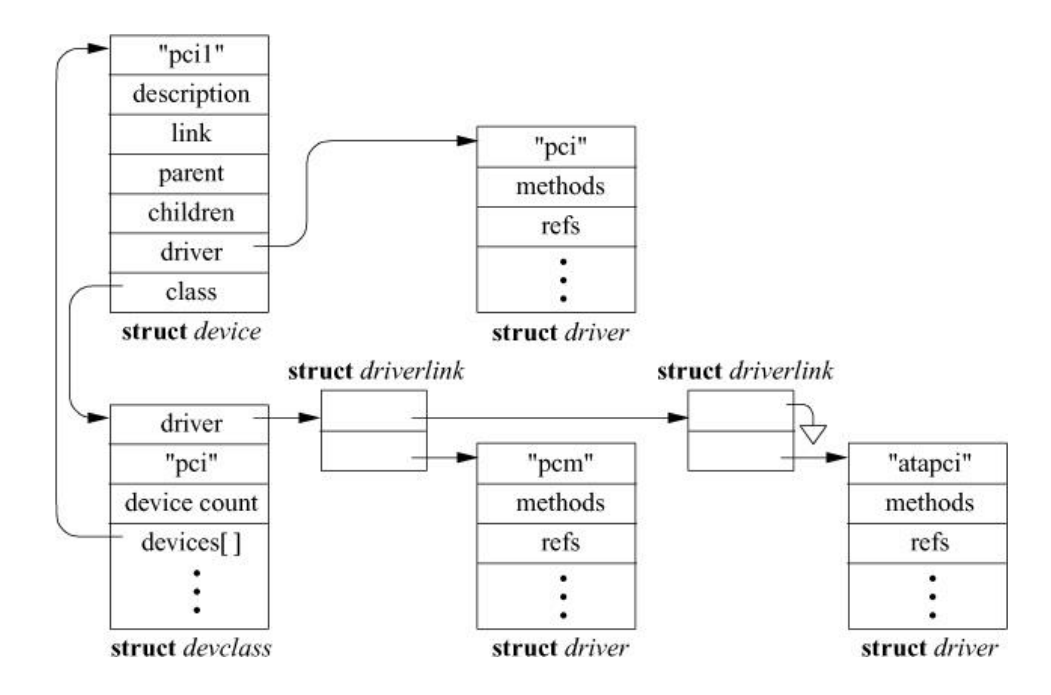
\includegraphics[width=\linewidth]{devclasses}
  \caption{Struktury devclasses \cite{image:freebsdbook1}.}
\end{center}
\end{figure}

Gdy urządzenie \textit{pci1} zidentyfikuje już wszystkie swoje dzieci, zaczyna przeprowadzać 
na nich dalsze etapy inicjalizacji.
Należy dobrać im sterowniki. Każde urządzenie spośród wszystkich sterowników w
klasie rodzica wybiera ten który pasuje najlepiej (względem wartości zwracanej podczas 
próbkowania sterowników; omówione w dalszej części pracy).
Nazwa urządzenia najczęściej ustawiana jest przez wybrany sterownik.
Np. przy dobraniu sterownika \textit{atapci} urządzeniu nadana zostanie nazwa \textit{atapci0}.
Kiedy sterownik został wybrany, urządzenie jest rejestrowane w klasie urządzeń o tej samej nazwie
co nazwa urządzenia. 

Taka klasa urządzeń zostanie utworzona na żądanie, chyba że została ona utworzona
na etapie \texttt{SI\_SUB\_DRIVERS}, ponieważ któryś sterownik przekazał właśnie taki
parametr w makrze \texttt{DRIVER\_MODULE}.

Rejestracja urządzenia w klasie urządzeń polega m.in. na zaalokowaniu następnego wolnego
numeru jednostkowego, który jest indeksem tego urządzenia w liście wskaźników na urządzenia w danej klasie
(pole \texttt{devices} w strukturze devclass). Pełną nazwą urządzenia będzie np. \textit{atapci0}.

% src: freebsd book
\begin{figure}
  \begin{center}
    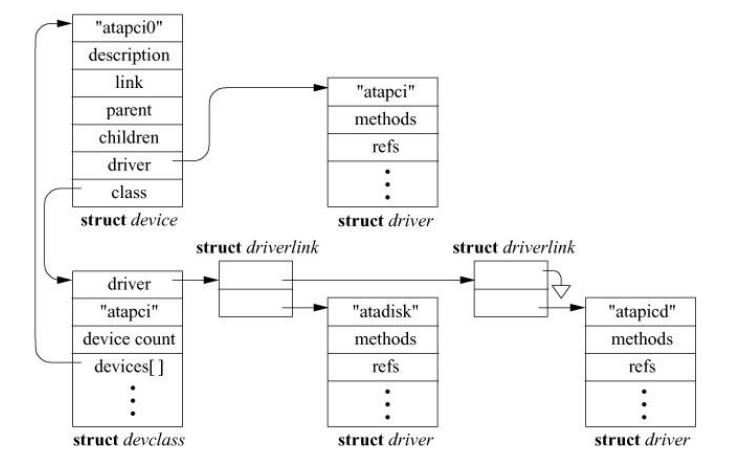
\includegraphics[width=\linewidth]{devclass2}
  \caption{Struktury devclasses \cite{image:freebsdbook2}.}
\end{center}
\end{figure}



Poniższe procedury są najbardziej podstawowymi procedurami związanymi z klasami urządzeń. 

\begin{lstlisting}
static devclass_t devclass_find_internal(const char *classname, 
                       const char *parentname, int create);

int devclass_add_driver(devclass_t dc, driver_t *driver, 
                    int pass, devclass_t *dcp);
\end{lstlisting}

% Find or create a device class.
% If a device class with the name classname exists, return it,
% otherwise if create is non-zero create and return a new device class.
% If parentname is non-NULL, the parent of the devclass is set to the devclass of that name.

% classname - the devclass name to find or create
% parentname - the parent devclass name or @c NULL
% create - non-zero to create a devclass

Pierwsza z tych procedur znajduje daną (\texttt{classname}) klasę urządzeń w systemie, bądź jeśli 
takiej nie znajdzie, może ją utworzyć (\texttt{create}). Znaleziona (bądź utworzona klasa),
jest podczepiana pod klasę rodzica (\texttt{parentname}), która jeśli nie istnieje również 
może zostać utworzona.

% int devclass_add_driver(devclass_t dc, driver_t *driver, int pass, devclass_t *dcp)
% 1118 * @brief Add a device driver to a device class
% 1119 *
% 1120 * Add a device driver to a devclass. This is normally called
% 1121 * automatically by DRIVER_MODULE(). The BUS_DRIVER_ADDED() method of
% 1122 * all devices in the devclass will be called to allow them to attempt
% 1123 * to re-probe any unmatched children.
% 1124 *
% 1125 * @param dc        the devclass to edit
% 1126 * @param driver    the driver to register
% 1127 */


Druga z procedur dodaje sterownik (\texttt{driver}) do danej klasy urządzeń (\texttt{dc}).
Klasa ta najczęściej jest klasą o nazwie równej parametrowi \texttt{busname} makra 
\texttt{DRIVER\_MODULE}. Ponadto inicjalizowana jest struktura devclass 
tego właśnie sterownika poprzez argument \texttt{dcp}.
W tej procedurze, również jak w poprzedniej, klasy urządzeń mogą być tworzone na żądanie
jeśli jeszcze nie istnieją.
Funkcja ta dodatkowo kompiluje sterownik jako obiekt w podsystemie \texttt{kobj}.

System posiada globalną listę klas urządzeń:\\
\texttt{static devclass\_list\_t devclasses = TAILQ\_HEAD\_INITIALIZER(devclasses);}


\begin{lstlisting}[caption=Struktura driverlink]
struct driverlink {
  kobj_class_t  driver;
  TAILQ_ENTRY(driverlink) link;  // lista sterowników w klasie
  int pass;  // zmienna używana w podsystemie buspasses
  TAILQ_ENTRY(driverlink) passlink;
};
\end{lstlisting}

Warte wspomnienia są też następujące funkcje:

\begin{lstlisting}
int devclass_add_device(devclass_t dc, device_t dev)
int devclass_alloc_unit(devclass_t dc, device_t dev, int *unitp)
\end{lstlisting}

Odpowiednio dodają urządzenie do danej klasy oraz wyznaczają i rezerwują 
odpowiedni numer urządzenia w danej klasie.





\section{Wstępna konfiguracja urządzeń} % JM

Etapy inicjalizacji systemu związane z infrastrukturą do zarządzania 
urządzeniami sprzętowymi i sterownikami to \texttt{SI\_SUB\_DRIVERS} i \texttt{SI\_SUB\_CONFIGURE}, 
w takiej właśnie kolejności.

\begin{lstlisting}[caption=Etapy inicjalizacji systemu]
enum sysinit_sub_id {
  ...
  SI_SUB_DRIVERS    = 0x3100000, /* inicjalizacja sterowników */
  SI_SUB_CONFIGURE  = 0x3800000, /* konfiguracja urządzeń */
  ...
}
\end{lstlisting}

Podczas etapu inicjalizacji \texttt{SI\_SUB\_DRIVERS} ładowane są moduły jądra jądra, które
zawierają kod sterowników. W pierwszej kolejności jest to kod sterownika urządzenia \texttt{root},
omówiony wcześniej.

Każdy moduł będący sterownikiem urządzenia sprzętowego wywołuje makro
\texttt{DRIVER\_MODULE(name, busname, driver, devclass, evh, arg)}. \\
Argument \texttt{busname} specyfikuje do jakiego typu urządzenia (np. magistrali, mostu) podłączone jest 
dane urządzenie. Sterownik trafi zatem do klasy urządzeń grupującej sterowniki obsługujące
urządzenia podłączane do urządzenia typu \texttt{busname}.
Argumenty evh i arg pozwalają przekazać \textbf{rozszerzający uchwyt zdarzeń modułu} i jego argument.


Makro to dalej rozwija się do makra
\texttt{EARLY\_DRIVER\_MODULE\_ORDERED(name, busname, driver, devclass, evh, arg, order, pass)},
z argumentem \texttt{order} [\ref{listing:elem_order}] równym \texttt{SI\_ORDER\_MIDDLE}.
Argument pass jest wartością
używaną w mechanizmie \texttt{buspasses}  omówionym w rozdziale \ref{sec:buspasses}.
Makro to definiuje następujące struktury: 

\begin{lstlisting}[caption=Makro EARLY\_DRIVER\_MODULE\_ORDERED]
#define EARLY_DRIVER_MODULE_ORDERED(name, busname, driver,    \
  devclass, evh, arg, order, pass)                            \
                                                              \
static                                                        \
struct driver_module_data name##_##busname##_driver_mod = {   \
  evh, arg,                                                   \
  #busname,                                                   \
  (kobj_class_t) &driver,                                     \
  &devclass,                                                  \
  pass                                                        \
};                                                            \
                                                              \
static moduledata_t name##_##busname##_mod = {                \
  #busname "/" #name,                                         \
  driver_module_handler,                                      \
  &name##_##busname##_driver_mod                              \
};                                                            \
DECLARE_MODULE(name##_##busname, name##_##busname##_mod,      \
  SI_SUB_DRIVERS,order)
\end{lstlisting}

\begin{lstlisting}[caption=Definicja struktury driver\_module\_data]
struct driver_module_data {
  int     (*dmd_chainevh)(struct module *, int, void *);
  void        *dmd_chainarg;
  const char  *dmd_busname;
  kobj_class_t    dmd_driver;
  devclass_t  *dmd_devclass;
  int     dmd_pass;
};
\end{lstlisting}

efektywnie czyniąc z kodu sterownika moduł jądra, a następnie wywołuje makro
\texttt{DECLARE\_MODULE(name\#\#\_\#\#busname, name\#\#\_\#\#busname\#\#\_mod, SI\_SUB\_DRIVERS, order)}
odpowiadające za zarejestrowanie modułu jądra w odpowiednim etapie inicjalizacji 
systemu [\ref{def:etapy_inicjalizacji}], czyli w \texttt{SI\_SUB\_DRIVERS}.


Podstawową rzeczą jaką system operacyjny musi wiedzieć o module jądra, to
jak wygląda \textbf{uchwyt zdarzeń modułu}.
W przypadku sterowników uchwyt zdarzeń modułu wygląda następująco:

\begin{lstlisting}
int
driver_module_handler(module_t mod, int what, void *arg)
{
  struct driver_module_data *dmd;
  devclass_t bus_devclass;
  kobj_class_t driver;
  int error = 0;
  int pass;

  dmd = (struct driver_module_data *)arg;
  bus_devclass = devclass_find_internal(dmd->dmd_busname, NULL, 
    TRUE);
    
  switch (what) {
  case MOD_LOAD:
    if (dmd->dmd_chainevh)
      error = dmd->dmd_chainevh(mod,what,dmd->dmd_chainarg);

    pass = dmd->dmd_pass;
    driver = dmd->dmd_driver;
    error = devclass_add_driver(bus_devclass, driver, pass, 
      dmd->dmd_devclass);
      break;
  case MOD_UNLOAD:
    error = devclass_delete_driver(bus_devclass, 
      dmd->dmd_driver);
    if (!error && dmd->dmd_chainevh)
      error = dmd->dmd_chainevh(mod,what,dmd->dmd_chainarg);
    break;
  case MOD_QUIESCE:
    ...
  }
  return (error);
}
\end{lstlisting}

Widzimy po uchwycie zdarzeń modułu sterowników, że główną operacją przy ładowaniu modułu sterownika
jest inicjalizacja \textbf{klas urządzeń (ang. devclasses} [\ref{sec:devclasses}], za pomocą
omówionych wcześniej procedur.
Najpierw znajdowana jest klasa urządzenia,
do której będzie podłączone urządzenie związane z tym sterownikiem. Następnie
sterownik ten dodawany jest do owej klasy, oraz jest kompilowany jako klasa kobj.
Również jeśli podana jest procedura rozszerzającego uchwytu zdarzeń modułu (\texttt{dmd\_chainevh}), 
jest ona wykonywana. Jest to procedura o takim samym prototypie jak uchwyt zdarzeń modułu, pozwala
rozszerzać standardową logikę przy ładowaniu sterownika.

Gdy moduł sterownika jest odczepiany, z odpowiedniej klasy urządzeń owy sterownik
jest usuwany. Dodatkowo może zostać wykonany rozszerzający uchwyt zdarzeń modułu.




\section{Przykładowe urządzenie} % JM

Pokażemy przykładową definicję sterownika kompletnie zmyślonego urządzenia - CFD (ang. Completely Fabricated Device),
która posłuży lepszej orientacji przy czytaniu następnych rozdziałów.

\begin{lstlisting}[caption=Szkielet kodu sterownika]
static int cfd_probe(device_t);
static int cfd_attach(device_t);
static int cfd_detach(device_t);
static int cfd_frob(device_t, int, int);
static int cfd_twiddle(device_t, char *);

static device_method_t cfd_methods[] = {
  /* Methods from the device interface */
  DEVMETHOD(device_probe, cfd_probe),
  DEVMETHOD(device_attach, cfd_attach),
  DEVMETHOD(device_detach, cfd_detach),

  /* Methods from the bogo interface */
  DEVMETHOD(bogo_frob, cfd_frob),
  DEVMETHOD(bogo_twiddle, cfd_twiddle),

  /* Terminate method list */
  DEVMETHOD_END
};

static driver_t cfd_driver = {
  "cfd",
  cfd_methods,
  sizeof(struct cfd_softc)
};

static devclass_t cfd_devclass;

DRIVER_MODULE(cfd, bogo, cfd_driver, cfd_devclass, NULL, NULL);
\end{lstlisting}

Każdy sterownik poza \texttt{root} wykorzystuje następujące makrodefinicje:
\texttt{\#define device\_method\_t     kobj\_method\_t;} \\
\texttt{\#define	DEVMETHOD	KOBJMETHOD}.

Powyższy kod można traktować jako minimalną implementację sterownika urządzenia sprzętowego.
Musi on implementować co najmniej procedury \texttt{probe}, \texttt{attach} i \texttt{detach} 
z interfejsu \texttt{device}. Zostaną one omówione przy omawianiu procesu autokonfiguracji [\ref{def:autoconf}].
Widzimy również, że urządzenie implementuje metody z hipotetycznego interfejsu \texttt{bogo}.
Mogą to być interfejsy \texttt{bus}, bądź specyficzne dla danej magistrali takie jak np. \texttt{pci}.
Niezbędna jest definicja struktury \texttt{driver\_t cfd\_driver}, oraz deklaracja
struktury \texttt{devclass\_t cfd\_devclass}, których adresy
są przekazywane za pomocą makra \texttt{DRIVER\_MODULE} podsystemowi sysinit.





\section{Interfejsy w sterownikach} % JM
\label{sec:interfaces}

Kod sterowników w większości opiera się na implementowaniu metod z różnych interfejsów
zrealizowanych za pomocą podsystemu kobj.

Bez interfejsów zmiana kodu sterownika mogłaby wymagać ponownej kompilacji innych części jądra. 
W dodatku modyfikacja jak i ponowna kompilacja niektórych przestarzałych sterowników może z różnych powodów
nie być już możliwa.
Z tych powodów stabilny interfejs jest kluczowy przy programowaniu sterowników.

Najważniejszym interfejsem, który muszą implementować wszystkie urządzenia
jest interfejs \texttt{device} będący trzonem podsystemu NewBus odpowiedzialnego za dopasowanie sterowników do
urządzeń i dalszą ich inicjalizację. Zostanie dokładniej omówiony w dalszej części pracy.

W kodzie sterowników urządzeń, definiowane są również obsługiwane procedury z innych interfejsów.
Na przykład interfejsem, który implementują szyny jest interfejs \texttt{bus}, opisany w pliku bus\_if.m
Istnieją także interfejsy specyficzne dla sterowników magistral konkretnego typu (np. PCI),
bądź inne definiowane przez programistę wedle uznania.

W interfejsach, dla niektórych metod zaimplementowane są wywołania dymyślne, jak i wywołania generyczne mające 
obsługiwać podstawowe przypadki.




\chapter{Autokonfiguracja}


\section{NewBus} % JM

% bridge devices create appropriate child bus devices.

Kiedy wszystkie sterowniki urządzeń są zarejestrowane w systemie, jądro przechodzi
do następnego etapu inicjalizacji [\ref{def:etapy_inicjalizacji}] - SI\_SUB\_CONFIGURE.
W tym etapie zachodzi proces zwany \textbf{autokonfiguracją}\label{def:autoconf}.

Podsystem NewBus zapewnia stabilny interfejs dla programistów sterowników urządzeń, oraz
szereg abstrakcji pozwalający w wygodny sposób przeprowadzać ich inicjalizację.
Zarządzanie urządzeniami jak i ich działanie również się upraszcza do wywoływania
odpowiednich metod z interfejsu.

W pliku \textit{autoconf.c}, zdefiniowane są trzy procedury odpowiadające za autokonfigurację:
\texttt{configure\_first}, \texttt{configure} i \texttt{configure\_final}.

\begin{lstlisting}[caption=Rejestracja procedur w podsystemie sysinit.]
SYSINIT(configure1, SI_SUB_CONFIGURE, SI_ORDER_FIRST, 
        configure_first, NULL);
SYSINIT(configure2, SI_SUB_CONFIGURE, SI_ORDER_THIRD, 
        configure, NULL);
SYSINIT(configure3, SI_SUB_CONFIGURE, SI_ORDER_ANY, 
        configure_final, NULL);
\end{lstlisting}

Pierwsza i trzecia z nich wykonują się odpowiednio przed i po skonfigurowaniu i utworzeniu drzewa urządzeń.
Zapewniają docelowemu procesowi autokonfiguracji pewne warunki wstępne jak i wykonują pewne operacje po
zakończeniu autokonfiguracji. Np. procedura \texttt{configure\_first} dodaje urządzenie \texttt{nexus}
jako dziecko urządzenia \texttt{root}.

Procedura \texttt{configure} jest punktem startowym autokonfiguracji.
Wywoływana jest procedura \texttt{root\_bus\_configure}, która następnie woła procedurę\\
\texttt{bus\_set\_pass(BUS\_PASS\_DEFAULT)} [\ref{sec:buspasses}] rozpoczynającą dynamiczne tworzenie \\
drzewa urządzeń, wraz z ich inicjalizacją.

W procesie konfiguracji urządzeń należy zidentyfikować wszystkie urządzenia w systemie jak i 
znaleźć odpowiadające im sterowniki. Jeżeli szyna/magistrala nie jest w stanie zidentyfikować
podłączonych do niej urządzeń, używa metody \texttt{identify} z interfejsu \texttt{device}.
Metoda ta identyfikuje (w zasadzie w dowolny sposób) i dodaje nowe urządzenie do danej szyny.
Niekiedy procedura ta po prostu zakłada, że dane urządzenie jest podłączone do systemu.

Sterownik każdego urządzenia sprzętowego musi implementować co najmniej metody \texttt{probe},
\texttt{attach}, oraz \texttt{detach} z interfejsu \texttt{device}.

Zidentyfikowane urządzenia podłączone do danej szyny są przekazywane do metody \texttt{probe}
sterowników w klasie urządzeń owej szyny. 

Metoda \texttt{probe} sterownika służy do sprawdzenia jaki stopień zgodności deklaruje on z danym urządzeniem.
System operacyjny wywołuję tę metodę, z danym urządzeniem jako argumentem, dla każdego sterownika w klasie urządzeń szyny
do której jest podłączony.
Sterownik którego metoda probe zwróciła największą wartość (mniejszą, bądź równą zero; 
wartości większe od 0 oznaczają błąd wykonania), jest wybierany jako najlepiej pasujący i przechodzi do
dalszego etapu konfiguracji. Proces ten w autorskim tłumaczeniu nazywamy \textbf{próbkowaniem}.
Jeżeli żaden ze sterowników nie zwrócił zadowalającej wartości, urządzenie nie jest obsługiwane.

\begin{lstlisting}[caption=Zwracane wartości probe]
#define BUS_PROBE_SPECIFIC  0  /* Sterownik specyficzny dla 
                                  danego urządzenia. */
#define BUS_PROBE_VENDOR   (-10) /* Sterownik dostarczony
                                    przez producenta. */
#define BUS_PROBE_DEFAULT   (-20)  /* Domyślny sterownik. */
#define BUS_PROBE_LOW_PRIORITY (-40) /* Starszy sterownik. */ 
#define BUS_PROBE_GENERIC  (-100)  /* Generyczny sterownik dla 
                                      danego typu urządzeń. */
#define BUS_PROBE_HOOVER   (-1000000) /* Sterownik obsługujący
                                         każde urządzenie danej
                                         magistrali. */
#define BUS_PROBE_NOWILDCARD  (-2000000000) // Brak dopasowania.
\end{lstlisting}

Kiedy najlepszy sterownik został odnaleziony, wywoływana jest jego metoda attach.
W metodzie tej dokonuje się właściwa inicjalizacja danego urządzenia, specyficzna dla niego.
Rezerwowane są zasoby i rejestrowane procedury obsługi przerwań.
Między innymi sterownik rezerwuje miejsce na prywatne dane danej instancji 
urządzenia (pole \texttt{softc} w strukturze \texttt{device\_t}) \cite{man:softc}.

Zadaniem szyny podczas attach, oprócz inicjalizacji samej siebie jest 
enumeracja podłączonych do niej urządzeń sprzętowych, utworzenie reprezentujących
je urządzeń programowych (struktur \texttt{device\_t}), a następnie wykonanie na nich sekwencji
probe i attach.
Procedurą realizującą tą sekwencję jest \texttt{bus\_generic\_attach} \cite{man:bus_generic_attach_9}.
Sterownik swoje prywatne dane może umieścić pod wskaźnikiem będącym polem \texttt{ivars} struktury \texttt{device\_t} \cite{man:ivars}.

% https://www.freebsd.org/cgi/man.cgi?query=bus_generic_attach&sektion=9&manpath=FreeBSD+11.2-RELEASE+and+Ports

Urządzenia nie posiadające podległych urządzeń są liśćmi w drzewie urządzeń i nie kontynuują procesu autokonfiguracji.



\section{Zarządzanie zasobami sprzętowymi} % WM
% https://www.freebsd.org/cgi/man.cgi?query=bus_alloc_resource&sektion=9&apropos=0&manpath=FreeBSD+11.2-RELEASE+and+Ports
% https://www.freebsd.org/cgi/man.cgi?query=rman_get_virtual&apropos=0&sektion=9&manpath=FreeBSD+9-current&format=html  
% http://bxr.su/FreeBSD/sys/kern/subr_rman.c


Urządzenia potrzebują zasobów, którymi najczęściej są obszary pamięci. Sterowniki w 
trakcie inicjalizacji urządzeń muszą zarezerwować zasoby oraz przypisać je do urządzeń. 

Rman - Resource Manager - Menadżer Zasobów jest abstrakcją pomagającą w zarządzaniu zasobami magistral, 
którymi najczęściej jest pamięć. Wprowadza ona dwa pojęcia - region, czyli ciągły zakres zasobów oraz zasób 
(resource) będący jednym z wielu fragmentów tego regionu.

Najpierw należy strukturę typu `rman` zainicjalizować - używając funkcji \\
\texttt{rman\_init(struct rman *rm)}, 
następnie przekazuje mu się region funkcją \\
\texttt{rman\_manage\_region(struct rman *rm, rman\_res\_t start, rman\_res\_t end)}.

Każda rezerwacja zasobu, o 
której można myśleć jak o alokacji, odbywa się za pomocą funkcji:
\begin{lstlisting}
rman_reserve_resource(struct rman *rm, rman_res_t start, 
  rman_res_t end, rman_res_t count, u_int flags, device_t dev));
\end{lstlisting}
lub funkcji z innym interfejsem. Wszystkie te funkcje mają wspólną implementację.

Za pomocą argumentów wspomnianej funkcji, możemy wyspecyfikować rozmiar zasobu (\texttt{count}), oraz oczekiwania 
dotyczące jego lokalizacji (\texttt{start}, \texttt{end}). Możemy podać dokładny adres, przedział, w którym zasób ma zostać 
zarezerwowany lub pozwolić na dowolny adres. 

Przez flagi możemy przekazać do jakiego rozmiaru ma być wyrównany adres. Możemy także nakazać, aby zasób był 
współdzielony, co jest potrzebne na przykład w przypadku magistrali 
ISA, gdzie wiele urządzeń dzieli tę samą pamięć.

Warto zauważyć, że jesteśmy w stanie wewnątrz zasobu utworzyć region, co tworzy drzewiastą 
strukturę. 

W idealnym świecie istniałby region obejmujący całą fizyczną przestrzeń adresową. 
Jednym z jej dzieci (lub wnuków albo nawet prawnuków) byłby zasób - pamięć na którą 
mapowane jest PCI. Ten zasób jednocześnie byłby regionem w którym zmapowane BARy PCI urządzeń. 
Jednym z tych urządzeń mógłby być kontroler innej magistrali. Urządzenie podłączone do niej byłoby 
w końcu liściem w tym drzewie.



Urządzenia nie mają dostępu do rmanów trzymanych przez szyny, 
do których są podczepione. Dlatego o zasoby muszą prosić poprzez metodę \texttt{bus\_alloc\_resource}, 
którą każdy sterownik magistrali implementuje osobno. Zazwyczaj jej działanie nie wybiega 
daleko poza zawołanie \texttt{rman\_reserve\_resource} w trzymanym przez siebie rmanie, 
lub zawołanie metody \texttt{bus\_alloc\_resource} u rodzica. 
W drugim przypadku można użyć gotowej metody \texttt{bus\_generic\_alloc\_resource}.


\section{Bus space} % WM
% https://www.freebsd.org/cgi/man.cgi?query=bus_space&manpath=FreeBSD+11.2-RELEASE+and+Ports
Jedno urządzenie może być podłączone na wiele różnych sposobów. Twórca sterownika nie wie, 
przez jakie szyny danych jest ono obsługiwane. 
Architektury komputera czasem wymuszają stosowanie 
MMIO, czasem PMIO. Z tego powodu systemy operacyjne oferują warstwę abstrakcji nad interakcją z 
pamięcią urządzenia, która we FreeBSD nazywa się \textbf{bus\_space} \cite{man:bus_space_9}. Pozwala ona na użycie dokładnie 
tego samego kodu sterownika, niezależnie od architektury i organizacji platformy sprzętowej.

\begin{lstlisting}
bus_space_map(tag, address, size, flags, handle_ptr)
\end{lstlisting}

Funkcja \texttt{bus\_space\_map} jako pierwszy argument bierze tag, który jednoznacznie wskazuje 
na typ przestrzeni adresowej, np MMIO lub PMIO w przypadku x86. W przypadku architektury MIPS, 
gdzie dostępne jest tylko MMIO, będzie dostępny tylko jeden tag. Funkcja ta 
tworzy uchwyt na zasób pod adresem `address` i rozmiarze `size`. 


\begin{lstlisting}
bus_space_read_1(tag, handle, offset)
bus_space_read_2(tag, handle, offset)
bus_space_read_4(tag, handle, offset)
bus_space_read_8(tag, handle, offset)

bus_space_write_1(tag, handle, offset, value)
bus_space_write_2(tag, handle, offset, value)
bus_space_write_4(tag, handle, offset, value)
bus_space_write_8(tag, handle, offset, value)
\end{lstlisting}

Powyższe funkcje pozwalają na zapis lub odczyt danych wielkości 1, 2, 4 lub 8 bajtów. Każda z nich 
jako argumenty bierze tag, wcześniej utworzony uchwyt oraz przesunięcie względem początku danego obszaru. 

Powyższe funkcje nie gwarantują wykonania w tej samej kolejności, co ich wywołania. 
W celu uczynienia operacji synchronicznymi, należy użyć funkcji:
\begin{lstlisting}
bus_space_barrier(space, handle, offset, length, flags)
\end{lstlisting}

Która jako jako flagi bierze jedną z poniższych wartości, lub obie:
\begin{lstlisting}
BUS_SPACE_BARRIER_READ 
BUS_SPACE_BARRIER_WRITE 
\end{lstlisting}

Zatrzymują one wykonanie kodu do momentu zakończenia wszystkich operacji danego typu. 

Wszystkie powyższe metody mają osobną implementację dla każdej architektury procesora. 
Na przykład w przypadku x86, funkcje \texttt{bus\_space\_write\_*}, bezpośrednio piszą do pamięci 
lub portów IO, zależnie od przekazanego taga jako pierwszy argument. W przypadku MIPSa i ARMa, 
wołany jest kod szyny, który w większości przypadków po prostu pisze pod dany adres pamięci.


\section{buspasses} % JM
\label{sec:buspasses}
% https://people.freebsd.org/~jhb/papers/bsdcan/2009/article.ps

Pierwotna implementacja podsystemu NewBus zakładała inicjalizację wszystkich
urządzeń za pomocą jednego przejścia (i jednoczesnego tworzenia) drzewiastej
hierarchii urządzeń. Podczas tego procesu każda szyna odpowiedzialna była
za zidentyfikowanie swoich dzieci i przekazanie dalej procesu inicjalizacji
do każdego z nich.

Mechanizm ten działa bardzo dobrze w przypadku urządzeń, które są inicjalizowane
zawsze przed urządzeniami które od nich zależą, np. reprezentacji magistral, bądź mostów.

Jednakże są odmienne przypadki.
Np. kontrolery przerwań, takie jak 8259A w architekturze x86.
Programowa reprezentacja tego kontrolera jest w hierarchii dzieckiem szyny ISA,
która z kolei jest dzieckiem mostu PCI-ISA, który podpięty jest do szyny PCI.
Inicjalizacja urządzeń podłączonych do szyny PCI będzie przeprowadzona wcześniej,
a one nierzadko korzystają z kontrolera przerwań.
Obejścia stosowane w takich wypadkach wprowadzają kod zależny od platformy,
poza podsystemem NewBus.


Rozwiązaniem powyższych problemów jest dodanie mechanizmu \textbf{buspasses} \cite{paper:buspasses}.
Zakłada on wielokrotne przechodzenie drzewa urządzeń i inicjalizowanie ich.
Sterownik może próbkować urządzenia wtedy i tylko wtedy, gdy nadany mu \textbf{pass level}
jest mniejszy niż ogólnosystemowy \textbf{pass level}.

Logika ta zaimplementowana jest w większości w procedurach \texttt{bus\_generic\_probe},
oraz \texttt{bus\_generic\_attach}.
Kiedy szyna wywołuje te metody, aby rozpocząć inicjalizację swoich dzieci, inicjalizacja
ta dokonywana jest tylko na tych które mają odpowiedni pass level.

System musi zarządzać poziomami pass level. Implementacja przejścia hierarchii
urządzeń musi być efektywna w przypadku rzadko rozłożonych poziomów pass level.
System trzyma więc listę aktywnych pass level - tych, które są niepuste.
Lista ta jest wyznaczana przy ładowaniu modułów sterowników (argument \texttt{pass} w makrze \texttt{DEVICE\_MODULE}). 
% Odnośnik do argumentu pass w makrze DEVICE_MODULE, opisane wyżej w pracy.
\newline
Aktualny poziom jest trzymany w globalnej zmiennej \texttt{bus\_current\_pass}.
Pass level może zostać zwiększony korzystając z procedury \texttt{bus\_set\_pass},
której wywołanie pośrednio powoduje ponowne przeskanowanie całego drzewa urządzeń z nowym poziomem pass level.
Podniesiony poziom nie może zostać zmniejszony. Powyższa procedura może powodować wielokrotne przejście
hierarchii urządzeń po kolei dla aktywnych pass levels, zatrzymuje się gdy lista aktywnych
będzie pusta, bądź natrafi na pass level wyższy niż aktualny. Wszystkie mniejsze niż
aktualny pass level są pomijane.

Ponowne przeskanowanie drzewa urządzeń dokonywane jest za pomocą procedury z interfejsu \texttt{bus}:
\texttt{bus\_new\_pass}. Istnieje również generyczna funkcja:\\\texttt{bus\_generic\_new\_pass}.
Procedura ta przejście całej hierarchii urządzeń od samego urządzenia root0.
Działa ona następująco: jeśli któreś z dzieci danego urządzenia używa nowego pass level, to
jego procedura identify jest wołana, i dodawany jest nowy pass level. Następnie jeśli
dziecko ma już dobrany sterownik, to wołana jest jego implementacja metody \texttt{bus\_new\_pass}.
W przeciwnym wypadku próbkowanie urządzenia wykonywane jest ponownie.


\begin{lstlisting}[caption=Poziomy pass level]
  #define BUS_PASS_ROOT       0   /* Używany przez root0. */
  #define BUS_PASS_BUS        10  /* Magistrale i mostki. */
  #define BUS_PASS_CPU        20  /* Urządzenia CPU. */
  #define BUS_PASS_RESOURCE   30  /* Enumeracja zasobów. */
  #define BUS_PASS_INTERRUPT  40  /* Kontrolery przerwań. */
  #define BUS_PASS_TIMER      50  /* Zegary. */
  #define BUS_PASS_SCHEDULER  60  /* Włączenie planisty. */
  #define BUS_PASS_DEFAULT    __INT_MAX /* Ostatni poziom. */
  
  #define BUS_PASS_ORDER_FIRST    0
  #define BUS_PASS_ORDER_EARLY    2
  #define BUS_PASS_ORDER_MIDDLE   5
  #define BUS_PASS_ORDER_LATE 7
  #define BUS_PASS_ORDER_LAST 9
\end{lstlisting}

Teraz kontrolery przerwań mogą normalnie uczestniczyć w inicjalizacji jako urządzenia
podsystemu NewBus, bez zbędnych obejść.


%%%%%%%%%%%%%%%%%%%%%%%%%%%%%%%%%%%%%%%%%%%%%%%%%%%%%%%%%%%%%%%%%%%%%%%%%%%%%%%%
% FREEBSD END
%%%%%%%%%%%%%%%%%%%%%%%%%%%%%%%%%%%%%%%%%%%%%%%%%%%%%%%%%%%%%%%%%%%%%%%%%%%%%%%%



\chapter{Mimiker}
Mimiker jest prostym unixo-podobnym systemem operacyjnym powstającym od listopada 2015 na naszej uczelni. 
Powstał tylko w celach edukacyjnych, bez ambicji na bycie lepszym od już istniejących systemów pisanych przez 
całe rzesze ekspertów. Duża część kodu naśladuje FreeBSD.
Mimiker jest dostępny na licencji BSD pod adresem \url{mimiker.ii.uni.wroc.pl}. W momencie pisania 
tego tekstu, lista kontrybutorów składa się z 19 osób.

Mimiker działa na platformie Malta z procesorem MIPS, której opis znajduje się w następnym rozdziale.
Przy rozwoju Mimikera nie używamy fizycznej płytki, lecz emulatora
Qemu, ponieważ jest to dla nas znacznie wygodniejsze. Quemu nie emuluje wszystkiego, co byśmy
chcieli, na przykład wyścigów między głównym potokiem procesora, a FPU.
Mimiker od dawna nie był testowany na prawdziwym sprzęcie i
najprawdopodobniej uruchomienie go na nim wymagałoby wielu poprawek.


W niedalekiej przyszłości chcemy zacząć wspierać platformy
wieloprocesorowe, a następnie przenieść system na architekturę ARM,
używając popularnej płytki Raspberry Pi. Od dłuższego czasu staramy się pisać kod
tak, aby jak najmniejsza jego ilość była zależna od platformy
sprzętowej, dzięki czemu tak duża zmiana, będzie wymagała przepisania
tylko niektórych mechanizmów. Polega to na wyraźnym oddzieleniu kodu 
specyficznego dla danej platformy - na przykład zapisu kontekstu wątku
przy przełączeniu - od kodu niezależnego od platformy - na przykład 
planisty systemowego.

\section{Płytka ewaluacyjna Malta} % WM
\label{sec:malta}
% http://wiki.prplfoundation.org/w/images/4/47/MD00627-2B-MALTA_R-USM-01.01.pdf
% https://www.linux-mips.org/wiki/MIPS_Malta

W celu umożliwienia pracy projektantom sprzętu oraz oprogramowania, nad 
mikroprocesorem, na rynku pojawiły się płytki ewaluacyjne. Są to obwody drukowane 
zawierające dany procesor, oraz współpracujące z nim komponenty, na przykład 
sprzętowy debugger, zegar czasu rzeczywistego, czy port szeregowy. Szczególnie 
na początku, płytki ewaluacyjne były dostarczane przez producenta danego 
mikroprocesora, ale nigdy nie było to regułą. Z czasem takie urządzenia zaczęły 
być wykorzystywane także przez hobbystów, co doprowadziło do powstania urządzeń 
o możliwościach daleko wybiegających poza pracę z samym procesorem. Zaczęły one 
przypominać kompletne komputery.



Malta jest już dosyć starą i trudną do zdobycia w dzisiejszych czasach
płytką ewaluacyjną w rozmiarze ATX, stworzoną przez firmę MIPS
Technologies w celu umożliwienia pracy nad układami mips32 i
mips64. Na płytce znajdziemy
kontrolery PCI, IDE, USB, zegar czasu rzeczywistego, most południowy
PIIX4, PS/2, ethernet.  Jest to bardzo popularny sprzęt (jak na tę
architekturę), wspierają ją systemy takie jak Linux, FreeBSD oraz
NetBSD.



\begin{figure}	
  \begin{center}	
    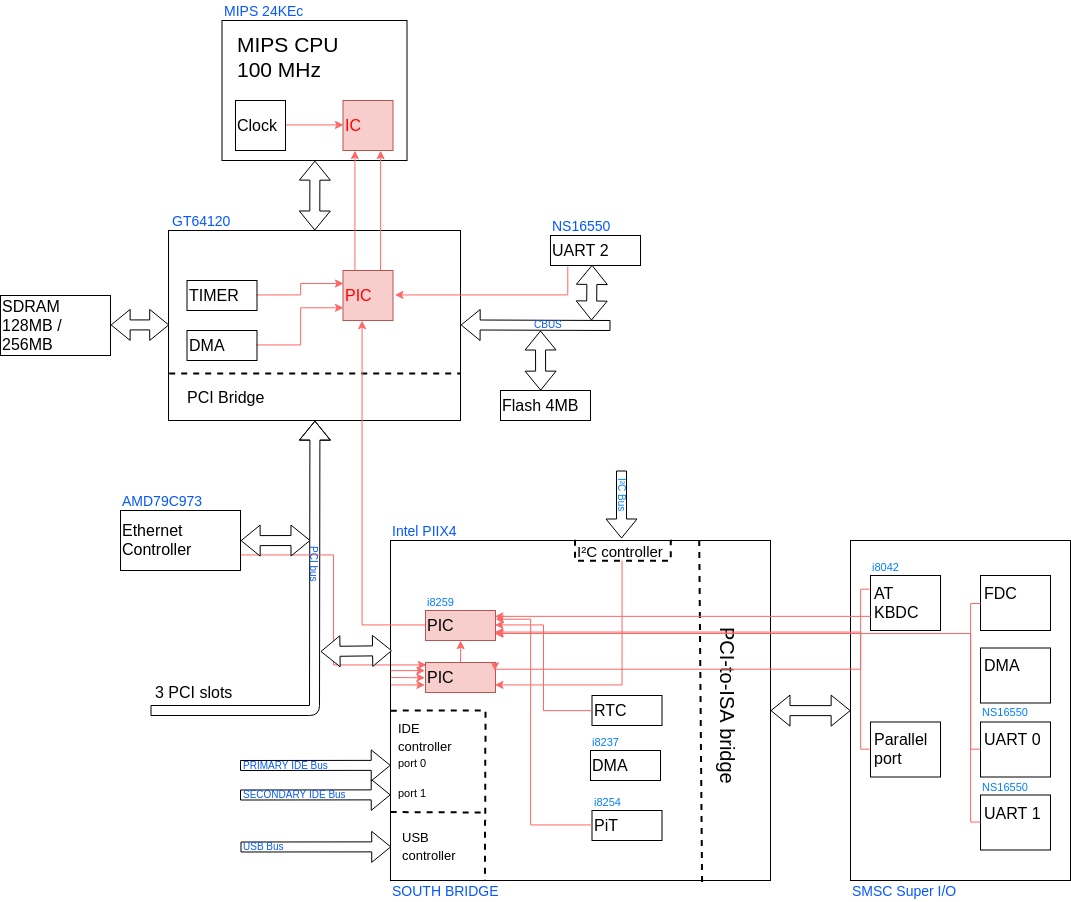
\includegraphics[width=\linewidth]{malta}	
  \caption{Platforma Malta}	
\end{center}	
\end{figure}

\section{MIPS} % WM
Architektura MIPS\cite{mips24k}, na której
pracujemy, kiedyś była używana w komputerach osobistych, najlepszych
superkomputerach, oraz konsolach do gier takich jak PlayStation 1,
PlayStation 2, PlayStation portable.  Dziś w większości została
wyparta przez architektury z rodziny x86 oraz ARM. Można ją nadal
znaleźć w systemach wbudowanych, na przykład w najtańszym sprzęcie
sieciowym.

Oryginalnie procesor był 32-bitowy, jednak powstały także wersje 64-bitowe. Jest
to architektura typu RISC, oraz load/store - czyli z możliwie prostymi
instrukcjami oraz z wyraźnym rozdzieleniem tych odpowiedzialnych za
interakcję z pamięcią od tych odpowiedzialnych za obliczenia. Z powodu
prostoty, często znajduje zastosowanie w celach edukacyjnych.

Specyficzny dla tej architektury jest Branch Delay Slot - zgodnie ze
specyfikacją, jedna instrukcja bezpośrednio po instrukcji skoku,
zostanie wykonana zawsze, nawet jeśli skok w inne miejsce się wykona.
Adresy instrukcji muszą być wyrównane do jej rozmiaru, czyli na
przykład czterobajtowa instrukcja nie może znajdować się pod adresem
kończącym się cyfrą 3, gdyż taki adres nie jest wielokrotnością liczby
4.

Procesory MIPS wspierają 4 koprocesory, czyli procesory
pomocnicze. Pierwszym z nich jest zawsze koprocesor systemowy,
który odpowiada za takie mechanizmy jak tłumaczenie adresów z
wirtualnych na fizyczne lub obsługa wyjątków. Drugim jest zazwyczaj
FPU, który nie jest jednak obowiązkowy. Pozostałe dwa nie są
zdefiniowane przez standard. Na przykład dodatkowym koprocesorem w
konsoli do gier PlayStation był odpowiedzialny za wspomaganie
obliczeń grafiki trójwymiarowej.


\section{Co dopisaliśmy} % JM / WM
% https://github.com/cahirwpz/mimiker/pull/447
Podczas pracy z Mimikerem zastaliśmy poważny problem, polegający na 
przydzielaniu BARom PCI adresów, które nachodziły na sztywno 
zmapowaną pamięć magistrali ISA.

Z pomocą przyszedł RMAN - bardzo podobny resource manager do opisanego wcześniej ale trochę prostszy.

Rezerwacja, nazwana u nas alokacją, odbywa się za pomocą funkcji:
\begin{lstlisting}
resource_t *
rman_alloc_resource(rman_t *rm, rman_addr_t start, 
  rman_addr_t end, size_t count, size_t bound, 
  res_flags_t flags, device_t *dev);
\end{lstlisting}

Cała implementacja resource managera zajmuje niewiele ponad 100 linii kodu. O każdej instancji struktury 
\texttt{rman\_t} możemy myśleć jak o liście zasobów (struktur \texttt{resource\_t}). 
Początkowo zawiera on jeden zasób odpowiadający całemu jego rozmiarowi. Każda alokacja znajduje 
pierwszy wolny zasób będący w stanie pomieścić rozmiar zadany jako argument i jeśli jest on większy, 
wykraja pozostałą część jako nowy zasób (w niektórych przypadkach nawet jako dwa zasoby - przed i za 
zaalokowanym). Ponadto możliwe jest wyspecyfikowanie, aby alokacja miała miejsce w konkretnym miejscu, 
za pomocą argumentów \texttt{start} i  \texttt{end}.

Alokacja zasobów współdzielonych nie jest obsługiwana, ponieważ struktura resource\_t zawiera 
wskaźnik na urządzenie. Współdzielony zasób musiałby wskazywać na wiele urządzeń - właścicieli, a to 
komplikuje implementację, która z założenia miała być bardzo prosta. 

Po wprowadzeniu kodu odpowiedzialnego za zarządzanie zasobami do Mimikera
należało wprowadzić do infrastruktury sterowników interfejs, który pozwalałby korzystać z kodu menedżera zasobów.
Zaimplementowaliśmy interfejs podobny do opisanego wcześniej interfejsu \texttt{bus\_*\_resource} 
z FreeBSD.
Uprościliśmy interfejs do jednej funkcji:
\begin{lstlisting}
resource_t *
bus_resource_alloc(device_t *dev, resource_type_t type, int rid,
  rman_addr_t start, rman_addr_t end, size_t size, 
  unsigned flags)
\end{lstlisting}

Użycie powyższej funkcji jest takie samo jak w analogicznej funkcji z FreeBSD omówionej we wcześniejszych
rozdziałach.

Naszym docelowym założeniem było, aby każdy dostęp do zasobów urządzeń był wykonywany poprzez
uzyskaną wcześniej za pomocą powyższej funkcji reprezentacją zasobu \texttt{resource\_t}.
Zasób ten pobierany był z menedżera zasobów nadrzędnej szyny. Podczas procesu konfiguracji
urządzeń i sterowników, każda szyna pobiera od rodzica (za pomocą bus\_resource\_alloc) 
odpowiedni zasób, którym inicjalizowany jest resource manager owej szyny. Z tego resource managera podrzędne
względem tej szyny urządzenia będą mogły prosić o zasoby. W związku z tym każda szyna,
której dzieci mogą prosić o zasoby musi implementować funkcję obsługującą takie żądanie i 
wyeksportować wskaźnik na nią w strukturze \texttt{bus\_methods\_t}.

Taki mechanizm pozwala na dynamiczne przydzielanie zasobów, oraz pozwala wykryć i uniknąć konfliktów 
przy ich przydzielaniu.

Napisany przez nas kod można znaleźć pod linkiem \url{https://github.com/cahirwpz/mimiker/pull/447}.


\chapter{Zalecana dalsza lektura} % WM
\begin{itemize}  
\item \textsc{Andrew S. Tanenbaum, Herbert Bos} - \textit{Systemy operacyjne} 
\item \textsc{Marshall Kirk McKusick, George V. Neville-Neil, Robert N.M. Watson} - \textit{The Design and Implementation of the FreeBSD Operating System}  
\item \textsc{Paul E. McKenney} - \textit{Memory Barriers: a Hardware View for Software Hackers}
\item \textsc{Joseph Kong} - \textit{FreeBSD Device Drivers: A Guide for the Intrepid}
\item \textsc{Alessandro Rubini, Jonathan Corbet} - \textit{Linux Device Drivers}
\item \textsc{Bruce Jacob, David T. Wang, Spencer W. Ng} - \textit{Memory Systems: Cache, DRAM, Disk}
\end{itemize}



%%%%% BIBLIOGRAFIA

\begin{thebibliography}{1}


\bibitem{paper:neumann} \textsc{John von Neumann}, 
\textit{First Draft of a Report on the EDVAC}

\bibitem{paper:buspasses} \textsc{John H. Baldwin}, 
\textit{Multiple Passes of the FreeBSD Device Tree},
\url{https://people.freebsd.org/~jhb/papers/bsdcan/2009/article.ps}

\bibitem{book:memory_systems_chapter_18} \textsc{Bruce Jacob, David T. Wang, Spencer W. Ng},
\textit{Memory Systems: Cache, DRAM, Disk}, rozdział 18

\bibitem{book:linux_device_drivers} \textsc{Alessandro Rubini, Jonathan Corbet},
\textit{Linux Device Drivers}, wydanie II, Using resources

\bibitem{book:tanenbaum_hardware} \textsc{Andrew S. Tanenbaum, Herbert Bos},
\textit{Systemy operacyjne}, wydanie IV, rozdział 1.3

\bibitem{book:tanenbaum_history} \textsc{Andrew S. Tanenbaum, Herbert Bos},
\textit{Systemy operacyjne}, wydanie IV, rozdział 1.2

\bibitem{book:tanenbaum_dyski} \textsc{Andrew S. Tanenbaum, Herbert Bos},
\textit{Systemy operacyjne}, wydanie IV, rozdział 1.3.3

\bibitem{paper:intrusive} \textsc{Jiri Soukup, Code Farms Inc.}, 
\textit{Intrusive Data Structures}

\bibitem{wiki:timesharing} \textsc{Wikipedia}, \textit{Time-sharing},
\url{https://en.wikipedia.org/wiki/Time-sharing}

\bibitem{wiki:neumann} \textsc{Wikipedia}, \textit{Von Neumann architecture},
\url{https://en.wikipedia.org/wiki/Von_Neumann_architecture}

\bibitem{wiki:batch_processing} \textsc{Wikipedia}, \textit{Batch processing},
\url{https://en.wikipedia.org/wiki/Batch_processing}

\bibitem{wiki:magistrala_def} \textsc{Wikipedia}, \textit{Magistrala komunikacyjna} ,
\url{https://pl.wikipedia.org/wiki/Magistrala_komunikacyjna}

\bibitem{wiki:point_point} \textsc{Wikipedia}, \textit{Point-to-point},
\url{https://en.wikipedia.org/wiki/Point-to-point_(telecommunications)}

\bibitem{scsi} \textsc{Wikipedia}, \textit{SCSI},
\url{https://en.wikipedia.org/wiki/SCSI}

\bibitem{ata_ide} \textsc{Wikipedia}, \textit{Parallel ATA},
\url{https://en.wikipedia.org/wiki/Parallel_ATA}

\bibitem{pcie} \textsc{Wikipedia}, \textit{PCI-express},
\url{https://en.wikipedia.org/wiki/PCI_Express}

\bibitem{pci_arbitration} \textsc{Wikipedia}, \textit{Conventional PCI - Arbitration},
\url{https://en.wikipedia.org/wiki/Conventional_PCI#Arbitration}

\bibitem{fsb} \textsc{Wikipedia}, \textit{Front Side Bus},
\url{https://en.wikipedia.org/wiki/Front-side_bus}

\bibitem{southbridge} \textsc{Wikipedia}, \textit{Southbridge (computing)},
\url{https://en.wikipedia.org/wiki/Southbridge_(computing)}

\bibitem{northbridge} \textsc{Wikipedia}, \textit{Northbridge (computing)},
\url{https://en.wikipedia.org/wiki/Northbridge_(computing)}

\bibitem{pleonazm} \textsc{Wikipedia}, \textit{Pleonazm},
\url{https://pl.wikipedia.org/wiki/Pleonazm}

\bibitem{wiki:lkm} \textsc{Wikipedia}, \textit{Loadable kernel module},
\url{https://en.wikipedia.org/wiki/Loadable_kernel_module}

\bibitem{wiki:controller} \textsc{Wikipedia}, \textit{Device controller},
\url{https://simple.wikipedia.org/wiki/Device_controller}

\bibitem{wiki:bus} \textsc{Wikipedia}, \textit{Bus (computing)},
\url{https://en.wikipedia.org/wiki/Bus_(computing)}

\bibitem{pcisig} \textsc{PCI-SIG},
\url{https://pcisig.com}

\bibitem{sata} \textit{Serial ATA International Organization (SATA-IO)},
\url{https://sata-io.org/}

\bibitem{rootkits} \textsc{Dino Dai Zovi}, \textit{Kernel Rootkits},
\url{https://www.sans.org/reading-room/whitepapers/threats/kernel-rootkits-449}

\bibitem{just2good} \textsc{Information Technology Resource and Forum Just2Good},
\textit{Introduction to the Chipset},
\url{http://just2good.co.uk/chipset.php}

\bibitem{hypertransport} \textsc{HyperTransport Consortium}, \textit{HyperTransport Overview},
\url{https://www.hypertransport.org/ht-overview}

\bibitem{quickpathinterconnect} \textsc{Intel}, \textit{An Introduction to the Intel® QuickPath Interconnect},
\url{https://www.intel.com/content/www/us/en/io/quickpath-technology/quick-path-interconnect-introduction-paper.html}

\bibitem{zasoby2} \textsc{Eli Billauer}, \textit{The Right Way: Managed Resource Allocation in
Linux Device Drivers},
\url{http://haifux.org/lectures/323/haifux-devres.pdf}

\bibitem{def:pio} \textsc{I/O Techniques}, \textit{Programmed I/O},
\url{http://inputoutput5822.weebly.com/programmed-io.html}

\bibitem{def:mmio} \textsc{Wikipedia}, \textit{Memory-mapped I/O},
\url{https://en.wikipedia.org/wiki/Memory-mapped_I/O}

\bibitem{Shichao's Notes} \textit{Interrupts and Interrupt Handlers},
\url{https://notes.shichao.io/lkd/ch7/}

\bibitem{8259a} \textsc{Intel}, \textit{8259A PROGRAMMABLE INTERRUPT CONTROLLER (8259A/8259A-2)},
\url{https://pdos.csail.mit.edu/6.828/2014/readings/hardware/8259A.pdf}

\bibitem{interrupts2} \textsc{jcm's blog}, \textit{Everything you know about interrupts is wrong},
\url{http://www.jonmasters.org/blog/2007/12/12/everything-you-know-about-interrupts-is-wrong/}

\bibitem{def:msi} \textsc{Wikipedia}, \textit{Message Signaled Interrupts},
\url{https://en.wikipedia.org/wiki/Message_Signaled_Interrupts}

\bibitem{def:apic} \textsc{Wikipedia}, \textit{Advanced Programmable Interrupt Controller},
\url{https://en.wikipedia.org/wiki/Advanced_Programmable_Interrupt_Controller}

\bibitem{def:wiki_dma} \textsc{Wikipedia}, \textit{Direct memory access},
\url{https://en.wikipedia.org/wiki/Direct_memory_access}

\bibitem{def:wiki_isa} \textsc{Wikipedia}, \textit{Industry Standard Architecture},
\url{https://en.wikipedia.org/wiki/Industry_Standard_Architecture}

\bibitem{usb} \textsc{Beyond Logic}, \textit{USB in a NutShell - Making sense of the USB standard},
\url{https://www.beyondlogic.org/usbnutshell/usb1.shtml}

\bibitem{def:wiki_plug_play} \textsc{Wikipedia}, \textit{Plug and Play},
\url{https://en.wikipedia.org/wiki/Plug_and_play}

\bibitem{def:wiki_legacy_pnp} \textsc{Wikipedia}, \textit{Legacy Plug and Play},
\url{https://en.wikipedia.org/wiki/Legacy_Plug_and_Play}

\bibitem{kobj_jake} Artykuł na temat podsystemu \texttt{kobj},
\url{https://people.freebsd.org/~jake/kobj/kobj.txt}

\bibitem{freebsd_handbook_kobj} \textit{FreeBSD Architecture Handbook},
rozdział 3.3: Kernel Objects - Using Kobj,
\url{https://www.freebsd.org/doc/en/books/arch-handbook/kernel-objects-using.html}

\bibitem{mips24k} \textit{MIPS32® 24K® Processor Core Family Software User’s Manual}, 
\url{https://people.freebsd.org/~adrian/mips/MD00343-2B-24K-SUM-03.11.pdf}

\bibitem{malta} \textit{MIPS® Malta™-R Development PlatformUser’s Manual}, 
\url{https://manualzz.com/doc/7240054/mips%C2%AE-malta%E2%84%A2-r-development-platform-user-s-manual}

\bibitem{cache_coherence} \textsc{Wikipedia}, \textit{Cache coherence},
\url{https://en.wikipedia.org/wiki/Cache_coherence}

\bibitem{wiki:bus_mastering} \textsc{Wikipedia}, \textit{Bus mastering},
\url{https://en.wikipedia.org/wiki/Bus_mastering}

\bibitem{pci_bus_mastering} \textsc{PC guide}, \textit{PCI Bus Mastering},
\url{http://www.pcguide.com/ref/mbsys/buses/types/pciMastering-c.html}

\bibitem{isa_bus_mastering} \textsc{Hardwarebook}, \textit{ISA},
\url{http://www.hardwarebook.info/ISA#Bus_Mastering}

\bibitem{wiki:bios} \textsc{Wikipedia}, \textit{BIOS},
\url{https://en.wikipedia.org/wiki/BIOS}

\bibitem{uefi} \textsc{Unified Extensible Firmware Interface Forum},
\url{http://www.uefi.org/}

\bibitem{mailing_list} Wątek listy mailingowej FreeBSD - \textit{Understanding the FreeBSD locking mechanism},
\url{https://groups.google.com/forum/#!topic/muc.lists.freebsd.hackers/FYk8EtGY-is}

\bibitem{bsd:smp_design} \textsc{FreeBSD Architecture Handbook},
\textit{SMP design},
\url{https://www.freebsd.org/doc/en/books/arch-handbook/smp-design.html}

\bibitem{queue_h} Kod źródłowy FreeBSD - plik \texttt{queue.h},
\url{http://fxr.watson.org/fxr/source/sys/queue.h?v=FREEBSD11}

\bibitem{tree_h} Kod źródłowy FreeBSD - plik \texttt{tree.h},
\url{http://fxr.watson.org/fxr/source/sys/tree.h?v=FREEBSD11}

\bibitem{resource_h} Kod źródłowy FreeBSD - plik \texttt{resource.h},
\url{http://fxr.watson.org/fxr/source/mips/include/resource.h?v=FREEBSD11}

\bibitem{freebsd:code_subr_bus} Kod źródłowy FreeBSD - plik \texttt{subr\_bus.c},
\url{http://fxr.watson.org/fxr/source/kern/subr_bus.c}

\bibitem{mips_intr_code} Kod źródłowy FreeBSD - plik \texttt{intr\_machdep.c},
\url{http://fxr.watson.org/fxr/source/mips/mips/intr_machdep.c}

\bibitem{mips_exception} Kod źródłowy FreeBSD - plik \texttt{exception.S},
\url{http://fxr.watson.org/fxr/source/mips/mips/exception.S}

\bibitem{image:von_neumann} Obrazek - uproszczony schemat architektury von Neumanna,
\url{https://commons.wikimedia.org/wiki/File:Von_Neumann_Architecture.svg}

\bibitem{image:system_bus} Obrazek - magistrala systemowa,
\url{https://commons.wikimedia.org/wiki/File:Computer_system_bus.svg}

\bibitem{image:south_north_bridges} Obrazek - architektura mostów północnego i południowego,
\url{https://commons.wikimedia.org/wiki/File:Motherboard_diagram.svg}

\bibitem{image:pch} \textsc{Andrew S. Tanenbaum, Herbert Bos},
\textit{Systemy operacyjne}, wydanie IV, rysunek 1.12

\bibitem{image:pci_config_space} Obrazek - przestrzeń konfiguracyjna PCI,
\url{https://commons.wikimedia.org/wiki/File:Pci-config-space.svg}

\bibitem{image:freebsdbook1} \textsc{Marshall Kirk McKusick, George V. Neville-Neil, Robert N.M. Watson},
\textit{The Design and Implementation of the FreeBSD Operating System},
wydanie II, rysunek 8.12

\bibitem{image:freebsdbook2} \textsc{Marshall Kirk McKusick, George V. Neville-Neil, Robert N.M. Watson},
\textit{The Design and Implementation of the FreeBSD Operating System},
wydanie II, rysunek 8.13

\bibitem{image:mostki} \textsc{The Linux Documentation Project}, \textit{PCI},
\url{https://www.tldp.org/LDP/tlk/dd/pci.html}


\bibitem{freebsd_book:tree} \textsc{Marshall Kirk McKusick, George V. Neville-Neil, Robert N.M. Watson},
\textit{The Design and Implementation of the FreeBSD Operating System},
wydanie II, listing 8.15



\bibitem{man:module_9} Podręcznik systemowy \texttt{module(9)},
\url{https://www.freebsd.org/cgi/man.cgi?query=module&sektion=9&manpath=FreeBSD+11.2-RELEASE+and+Ports}

\bibitem{man:malloc_9} Podręcznik systemowy \texttt{malloc(9)},
\url{https://www.freebsd.org/cgi/man.cgi?query=malloc&sektion=9&manpath=FreeBSD+11.2-RELEASE+and+Ports}

\bibitem{man:driver_9} Podręcznik systemowy \texttt{driver(9)},
\url{https://www.freebsd.org/cgi/man.cgi?query=driver&sektion=9&manpath=FreeBSD+11.2-RELEASE+and+Ports}

\bibitem{man:sysinit_9} Podręcznik systemowy \texttt{sysinit(9)},
\url{https://www.freebsd.org/cgi/man.cgi?query=SYSINIT&sektion=9&manpath=FreeBSD+11.2-RELEASE+and+Ports}

\bibitem{man:device_9} Podręcznik systemowy \texttt{device(9)},
\url{https://www.freebsd.org/cgi/man.cgi?query=device&sektion=9&manpath=FreeBSD+11.2-RELEASE+and+Ports}

\bibitem{man:devctl_8} Podręcznik systemowy \texttt{devctl(8)},
\url{https://www.freebsd.org/cgi/man.cgi?query=devctl&sektion=8&manpath=FreeBSD+11.2-RELEASE+and+Ports}

\bibitem{man:devctl_3} Podręcznik systemowy \texttt{devctl(3)},
\url{https://www.freebsd.org/cgi/man.cgi?query=devctl&sektion=3&manpath=FreeBSD+11.2-RELEASE+and+Ports}

\bibitem{man:sysctl_8} Podręcznik systemowy \texttt{sysctl(8)},
\url{https://www.freebsd.org/cgi/man.cgi?query=sysctl&sektion=8&manpath=FreeBSD+11.2-RELEASE+and+Ports}

\bibitem{man:sysctl_3} Podręcznik systemowy \texttt{sysctl(3)},
\url{https://www.freebsd.org/cgi/man.cgi?query=sysctl&sektion=3&manpath=FreeBSD+11.2-RELEASE+and+Ports}

\bibitem{man:devclass_9} Podręcznik systemowy \texttt{devclass(9)},
\url{https://www.freebsd.org/cgi/man.cgi?query=devclass&sektion=9&manpath=FreeBSD+11.2-RELEASE+and+Ports}

\bibitem{man:bus_generic_attach_9} Podręcznik systemowy \texttt{bus\_generic\_attach(9)},
\url{https://www.freebsd.org/cgi/man.cgi?query=bus_generic_attach&sektion=9&manpath=FreeBSD+11.2-RELEASE+and+Ports}

\bibitem{man:device.hints_5} Podręcznik systemowy \texttt{device.hints(5)},
\url{https://www.freebsd.org/cgi/man.cgi?query=device.hints&sektion=5&manpath=FreeBSD+11.2-RELEASE+and+Ports}

\bibitem{man:kobj_9} Podręcznik systemowy \texttt{kobj(9)},
\url{https://www.freebsd.org/cgi/man.cgi?query=kobj&sektion=9&manpath=FreeBSD+11.2-RELEASE+and+Ports}

\bibitem{man:bus_space_9} Podręcznik systemowy \texttt{bus\_space(9)},
\url{https://www.freebsd.org/cgi/man.cgi?query=bus_space&manpath=FreeBSD+11.2-RELEASE+and+Ports}

\bibitem{man:queue_3} Podręcznik systemowy \texttt{queue(3)},
\url{https://www.freebsd.org/cgi/man.cgi?query=queue&sektion=3&manpath=FreeBSD+11.2-RELEASE+and+Ports}

\bibitem{man:locking_9} Podręcznik systemowy \texttt{locking(9)},
\url{https://www.freebsd.org/cgi/man.cgi?query=locking&sektion=9&manpath=FreeBSD+11.2-RELEASE+and+Ports}

\bibitem{man:ithread_9} Podręcznik systemowy \texttt{ithread(9)},
\url{https://www.freebsd.org/cgi/man.cgi?query=ithread&sektion=9&manpath=FreeBSD+10.0-RELEASE}

\bibitem{man:bus_setup_intr_9} Podręcznik systemowy \texttt{bus\_setup\_intr(9)},
\url{https://www.freebsd.org/cgi/man.cgi?query=bus_setup_intr&manpath=FreeBSD+11.2-RELEASE+and+Ports}

\bibitem{man:critical_enter_9} Podręcznik systemowy \texttt{critical\_enter(9)},
\url{https://www.freebsd.org/cgi/man.cgi?query=critical_enter&sektion=9&manpath=FreeBSD+11.2-RELEASE+and+Ports}

\bibitem{man:ivars} Podręcznik systemowy \texttt{device\_set\_ivars(9)},
\url{https://www.freebsd.org/cgi/man.cgi?query=device_set_ivars&sektion=9&manpath=FreeBSD+11.2-RELEASE+and+Ports}

\bibitem{man:softc} Podręcznik systemowy \texttt{device\_get\_softc(9)},
\url{https://www.freebsd.org/cgi/man.cgi?query=device_get_softc&sektion=9&manpath=FreeBSD+11.2-RELEASE+and+Ports}

\bibitem{man:device_busy_9} Podręcznik systemowy \texttt{device\_busy(9)},
\url{https://www.freebsd.org/cgi/man.cgi?query=device_busy&sektion=9&manpath=FreeBSD+11.2-RELEASE+and+Ports}

\end{thebibliography}

\end{document}
